\documentclass[table]{report}
\usepackage{graphicx}
\usepackage{booktabs}
\usepackage{multirow}
\usepackage{amsmath}
\usepackage{float}
\usepackage{placeins}
\usepackage{array}     % For better column control
\usepackage{geometry}
% Required packages (add to preamble)
\usepackage{fancyhdr}  % For header/footer styling
\usepackage{setspace}  % For line spacing
\usepackage[hidelinks]{hyperref}  % For hyperlinks and \phantomsection
\usepackage[backend=biber]{biblatex}
\addbibresource{references.bib}
\usepackage{makeidx}  
% \usepackage{caption}  % For \captionof command
\usepackage[nottoc,notlot,notlof]{tocbibind} % Adds References to TOC
\usepackage[utf8]{inputenc}
\usepackage{textgreek} % for Greek letters in text
\usepackage{tikz}
\usepackage{arydshln} % add this in your preamble
\usetikzlibrary{arrows.meta, positioning}
\usepackage{pdfpages}
\tikzset{
  block/.style = {rectangle, draw, rounded corners, minimum height=1cm, minimum width=2.8cm, align=center},
  arrow/.style = {->, thick, >=Stealth},
}

\makeindex                  % Initializes index
\geometry{a4paper, margin=1in, bottom = 3.5cm}
\usepackage[table]{xcolor}
\definecolor{myblue}{RGB}{31,119,180}
\definecolor{dodgerblue}{RGB}{30,144,255}
\definecolor{darkgreen}{RGB}{0,100,0}


% Page formatting
\addtolength{\textwidth}{0mm}
\addtolength{\textheight}{12mm}
\addtolength{\topmargin}{-5mm}
\pretolerance = 10000000
\setlength{\parindent}{0pt}
\setlength{\parskip}{\baselineskip}
\onehalfspacing   
 
% Header / footer
\pagestyle{fancy}
\lhead{Manvendra Kumar Mishra, 201911048}
\chead{}
\rhead{\em MATH5872M, Dissertation in Data Science and Analytics}
\lfoot{}
\cfoot{\thepage}
\rfoot{}
\setlength{\headheight}{30pt}
\setlength{\footskip}{30pt}
\renewcommand{\headrulewidth}{0.6pt}
\renewcommand{\footrulewidth}{0pt}


\title{Machine Learning in Radio Spectrum Management}
\author{Manvendra Kumar Mishra}
\date{\today}

\begin{document}


\begin{titlepage}
    \centering
    
    \vspace*{3cm}
    {\LARGE \textbf{Machine Learning in Radio Spectrum Management} \par}
    
    \vspace{5cm}
    {\large Manvendra Kumar Mishra \par}
    {\large 201911048 \par}
    
    \vspace{2cm}
    {\large Supervised by Luisa Cuttilio \par}
    
    \vfill
    Submitted in accordance with the requirements for the \\
    module MATH5872M: Dissertation in Data Science and Analytics \\
    as part of the degree of \\
    
    \vspace{0.5cm}
    {\Large Master of Science in Data Science and Analytics \par}
    
    \vspace{0.5cm}
    The University of Leeds, School of Mathematics \par
    
    \vspace{0.5cm}
    \today\par
    
    \vspace{1.5cm}
    \begin{spacing}{1.1}
    \small The candidate confirms that the work submitted is his/her own and that appropriate credit has been given where reference has been made to the work of others. \\
    
    \vspace{0.3cm}
    Remember to include in here a signed and scanned pdf copy of your academic integrity form.
    \end{spacing}
    
\end{titlepage}

\pagenumbering{roman}
\clearpage

\includepdf[pages=-]{IntegrityDeclaration.pdf}
\clearpage

\begin{abstract}

This dissertation report presents the use of machine learning techniques to implement radiowave propagation management (prediction) in a data driven manner. A large-scale data set (449 MHz - 5.8  GHz) with multiple sites and frequency bands is being processed with feature scaling, site based embeddings and systematic data validation. To evaluate generalization capability of the models, neural networks as well as some baseline models such as linear regression, random forest, and XGBoost were trained and tested on site separated splits. Additionally, Random Forest model is trained at frequency as well as frequency-site level to compare the results with the deep neural network model.

Our neural network has always performed the best (MAE = 8.82 dB, MSE = 117.96) compared with traditional models (MAE $\geq 9.88$, MSE $\geq 155.02$). RMSE did not exceed 2.5–3.2 dB and R\^2 $\geq 0.95$ for all frequencies, reflecting the accuracy of hits and explained variance. The lowest bands (449 MHz) achieved the highest accuracy due to less attenuation by the environment, whereas higher bands showed slightly higher errors, but nevertheless exhibited strong prediction capacity. As a result, the validation and test results remained closely together which confirms that the model is generalizable and overfitting is not occurring.

The results show that neural networks offer a robust and scalable solution for radio-wave propagation prediction, comparison to empirical and ensemble approaches. Potential future improvements include the addition of frequency and site level separate model segregation, addition of topography information, a more systematic approach to addressing outliers, and a re-structuring of the deep learning architectures at finer scales (e.g., frequency- or site-specific). Such improvements would contribute to greater model robustness and applicability for practical communication network design.
\end{abstract}
\clearpage
\tableofcontents
\clearpage
\listoffigures        % Generates List of Figures
\clearpage
\listoftables         % Generates List of Tables
\clearpage

\pagenumbering{arabic} 
% ------------Introduction Section -----------------
\chapter{Introduction}

\section{Background and Motivation}

In the world of science and technology where majority of equipment requires network to connect with, having a safe and efficient network connection is just more than a basic requirement for survival. Now a days we have moved to 5G (faster connection), it is important for the service providers to make sure the radio network planning and spectrum management is to be their top priority. 

Radio network planning and spectrum management requires received signal level predictions that are a compromise between accuracy and computational efficiency. Spectrum Management, which provides a framework for the allocation of frequency bands to different types of utilizes various empirical propagation models, which are computationally efficient but often are too broad to capture the complex local effects that can impact link/network performance. On the other hand, deterministic models which are site specific and considered reliable in each environment is too complex to implement in all possible locations, and even if this was possible it is not easy to see the generic implications for spectrum sharing. An expert opinion is usually required at multiple stages of any spectrum sharing study. Machine learning is considered a promising approach to resolve the dichotomy between accuracy and efficiency. 

Thus, need of a generalized model is required to have which can counter the gaps between both Spectral Management and deterministic model and provides accurate results in terms of both speed and accuracy of the frequency / signals. 


\section{Aim and Objectives}
As per the project description, the aim of this report is to access the Ofcom’s open data of radio wave propagation across different sites in United Kingdom including (Boston, London, Merthyr, Nottingham, Scarhill, Southampton and Stevenage) and try to predict the signal loss or local mean measurement value. Using different machine learning methods. Evaluate this prediction accuracy across different environment and access the values for spectrum sharing. Share the results with Transfinite team to use the model in case seem fit for business requirement.

\section{Scope and Limitations}
While the data present is sufficient enough for a model to train and validate more accurately and cover most of the regions and frequencies, this still does not cover complete spectrum of area and frequencies. Additionally, the way data is captured is specific to a certain time duration and seasonality can also cause the difference in the signal strength, which is not captured in the current set of records.

\section{Report Structure}
In this report, a comprehensive survey on signal propagation modeling via machine learning is provided. The work is inspired by the increasing demand of accurate propagation prediction to design efficient wireless communication networks and to organize spectrum usage. \textbf{An introduction} which gives an understanding of what the research is all about, and keeping the reader in context of the study while also showing the aim and objectives, the scope as well as broad definition of terms.

\textbf{Literature Review} related works in propagation modeling, spectrum management issues and proposals, as well as the use of machine learning for propagation prediction. It also 9 highlights the limitations inherent in these current methods and research opportunities for which this study attempts to answer. After that, \textbf{Data Description \& Processing} introduces the dataset we use in this analysis, which includes data acquisition framework, schema, metadata and pre-processing. This chapter provides the reader with the foundation to the analysis and modeling that follows.

\textbf{Exploratory Data Analysis} is devoted to the exploratory data analysis where data distributions are considered, distances between TXs and RXs are estimated, and spatial dependence of the signal strength is analyzed. In \textbf{Methodology}, we show the methodology (model selection, formulation and implantation of Random Forest and Deep Learning models) and the evaluation metrics considered. \textbf{Model Selection and Justification} further compare the model results and select the best model for business purposes. Finally, \textbf{Conclusion} ends out study, summarizes findings, and \textbf{Future Enhancements} provides an outlook on possible future improvements and research.




\section{Key Definitions / Glossary}

\begin{enumerate}
  \item \textbf{Artificial Neural Networks (ANNs)}  
  
    ANNs are computational models inspired by the structure and function of biological neural networks. They consist of layers of interconnected nodes (neurons) that transform inputs through weighted connections and nonlinear activation functions, enabling them to approximate complex, non-linear functions \cite{goodfellow2016deep}.  


  \item \textbf{ConvNets (Convolutional Neural Networks)} 
  
  Neural networks using convolutional layers to extract spatially structured features—commonly used in image and signal processing.

  \item \textbf{Empirical Propagation Models:}  
  
    Empirical models such as \textit{COST-231} and \textit{Hata} are classical radio wave propagation models that estimate signal path loss based on measurement-driven formulas. The Hata model extends the Okumura model for urban, suburban, and rural environments, while COST-231 is an extension designed for higher frequency bands up to 2~GHz, making them widely used benchmarks in wireless network planning \cite{hata1980empirical, cost2311999}.  

  \item \textbf{Gaussian Mixture Model (GMM, Bayesian GMM)}
  
  A probabilistic model representing data as a weighted sum of Gaussian distributions; Bayesian GMMs introduce priors over parameters. Useful for clustering and channel MPC modeling \parencite{GMMsurvey,StanfordGMM}.

  \item \textbf{HF-band}
  
  High Frequency radio band: 3--30 MHz.

  \item \textbf{ITU recommendations}
  
  Standards and technical specifications by the International Telecommunication Union (e.g., IMT-2020 for 5G, IMT-2030 for 6G) \parencite{saad2019vision_6g}.

  \item \textbf{LSTM (Long Short-Term Memory)}
  
  A recurrent neural network (RNN) variant designed to capture long-range dependencies using gated memory cells. Commonly applied in sequence modeling.

  \item \textbf{ML (Machine Learning)}
  
  A field of AI where algorithms learn patterns from data to make predictions or decisions.

  \item \textbf{MLP (Multi-Layer Perceptron)}
  
  A feedforward artificial neural network with multiple fully connected layers, used for classification and regression.

  \item \textbf{MIMO arrays (Multiple-Input Multiple-Output)}
  
  Antenna systems with multiple transmitters (TXs) and receivers (RXs), improving spectral efficiency via spatial multiplexing or diversity \parencite{akbar2025survey_6g}.

  \item \textbf{mmWave (millimeter wave) and THz (Terahertz)}
  
  mmWave refers to frequencies between 30--300 GHz, used in 5G for high-capacity short-range communications. THz frequencies (>100 GHz) are a target band for 6G ultra-broadband systems \parencite{seker2021review_5g,akbar2025survey_6g}.

  \item \textbf{MPC clustering (Multipath Component clustering)}
  
  Grouping of propagation paths into clusters based on delay, angle, or other similarity measures for channel modeling.

  \item \textbf{Noise Floor}
  
  The baseline level of background noise in a system, below which signals cannot be reliably detected.

  \item \textbf{Q-band}
  
  Microwave band approximately 33--50 GHz, used for satellite and experimental communications.

  \item \textbf{RF plane-wave propagation}
  
  A propagation assumption where electromagnetic waves are modeled with planar wavefronts, valid in far-field regions.

  \item \textbf{Saliency Maps}
  
    Saliency maps are a visualization technique that highlight which parts of the input data (e.g., pixels in an image, or features in structured data) most influence the model’s prediction. In the context of neural networks, they help interpret the decision-making process by computing the gradient of the output with respect to the input features \cite{simonyan2014deep}.  
    

  \item \textbf{SHAP (Shapley Additive explanations)}  
  
    SHAP is a unified approach to explain the output of machine learning models by attributing the prediction to each input feature using concepts from cooperative game theory. It provides consistent and locally accurate explanations of feature importance \cite{lundberg2017shap}.  

  \item \textbf{Stochastic modeling}
  
  Channel modeling approach based on probabilistic/statistical descriptions of propagation variability, e.g., geometry-based stochastic models \parencite{seker2021review_5g}.

  \item \textbf{TXs \& RXs}
  
  TXs = Transmitters, RXs = Receivers.

  \item \textbf{3GPP baselines}
  
  Standardized baseline channel models developed by the 3rd Generation Partnership Project, combining deterministic and stochastic methods \parencite{seker2021review_5g}.

  \item \textbf{5G and 6G networks}
  
  5G = Fifth-Generation; 6G = Sixth-Generation wireless networks. 5G emphasizes mmWave and MIMO; 6G extends to THz, AI integration, and ultra-low latency \parencite{seker2021review_5g,akbar2025survey_6g,saad2019vision_6g}.

\end{enumerate}

% path loss theory

% ------------Literature Section -----------------
\clearpage
\chapter{Literature Review}

\section{Propagation Modeling Overview}

Propagation modeling is the foundation of wireless systems design and optimization. Classical methods can generally be divided into deterministic methods (probability-free) which are based upon Maxwell’s equations and RF plane-wave propagation, and statistical methods, which depend on empirical channel sounding across various environments.\parencite{huang2022artificial}. However, as networks evolve to 5G and 6G, propagation environments become increasingly complex. Large bandwidths, massive MIMO arrays, and higher frequency bands such as mmWave and THz require models that can capture site-specific variability and non-stationary channel characteristics \parencite{seretis2022overview}

Radio propagation and channel characterization have been evolving over the years. Characterizations based on propagation mechanisms and approximations to Maxwell’s equations or related laws of physics are usually considered as deterministic approaches. These models need to be validated with measurements and are useful for system deployments. Characterizations based on statistical descriptions of the channel responses are usually considered as statistical approaches,
being mainly based on channel measurements taken over multiple representative spatial/temporal/spectral samples in a given environment (e.g., urban, rural, and indoor office).
Combining the deterministic and stochastic approaches, geometry-based stochastic modeling has been developed to better characterize radio propagation channels. This approach utilizes greatly simplified ray tracing as well as measurement data for parameterization and validation \parencite{steinbauer2001doubledirectional}, \parencite{molisch2009cognitive}.

\section{Spectrum Management Challenges}

If the demand for wireless is increasing at an exponential rate, managing and employing the radio spectrum has become a growing concern. ”Traditional models, based on the planning criteria, such as ITU recommendations, are not adequate in dynamic environments\parencite{huang2021geometry}. To solve this, there have been proposed ML methods. For instance, \textbf{Wang et al.}\parencite{wang2022regional} designed ML models for HF-band frequency usability prediction which achieve more than 1 MHz lower RMS errors against ITU standards, providing a more accurate long-term spectrum planning. Similarly, \textbf{Bai et al.}\parencite{bai2022atmosphere} presented the neural network (NN) models for Q-band satellite channels and showed that they can be effectively used to predict the path loss of Q-band satellite channels possibly resulting in better utilization of the satellite spectrum.

The issues are more severe for higher frequencies. Path loss (especially at mmWave and THz), blockage, and environmental sensitivity all impact propagation\parencite{seretis2022overview}. \textbf{Gupta et al.}\parencite{gupta2022machine} tackled this in urban canyon scenarios by enriching lidar based street clutter data with CNN-based prediction models, and achieved notable improvements in path loss assessment over 3G baselines. These studies demonstrate that spectrum management in beyond 5G and 6G networks is only possible with intelligent, adaptive, and data-driven propagation models, which can adjust in a dynamic fashion depending on the environment.

\section{Machine Learning Practices in Propagation Prediction}

Machine learning has been commonly used to address the propagation prediction problem because it can consider the nonlinearities and high-dimensional dependencies. Applications include:

\begin{itemize}
    \item \textbf{MPC clustering:} In \textbf{Du et al.}\parencite{du2022svm} proposed an SVM (Support Vector Machine)-assisted adaptive kernel power density (AKPD) method for robust mmWave clustering by achieving a better performance than traditional techniques. Similarly, \textbf{Zhou et al.}\parencite{zhou2022machine} employed variational Bayesian GMM (Gaussian Mixture Model) for clustering in high speed rail applications and separated the static and dynamic features of the clusters.
    
    \item \textbf{Satellite and Atmospheric Channel Modeling:} \textbf{Bai et al.}\parencite{bai2022atmosphere} used MLP (Multilayer Perceptron) and LSTM (Long Short-Term Memory) networks to predict Q-band attenuation in real time and obtained good alignment with measured data.
    \item \textbf{Hybrid Physics-ML Models:} \textbf{Zhang et al.}\parencite{zhang2022predictive} proposed a hybrid ANN (Artificial Neural Network) + physics-based model for vegetation penetration at 28 GHz frequency, showing an improved accuracy in generalization respect to classical statistical models.
    \item \textbf{Urban Canyon and Outdoor Prediction:} \textbf{Gupta et.}\parencite{gupta2022machine} proposed a fusion of the lidar-based features and 3D building meshes in combination with ML models in order to minimize the RMSE (Root Mean Squared Error) of path loss prediction below 5 dB. \textbf{Liu et al.}\parencite{liu20223.5} also demonstrated that cheap geographical information would support acceptable RSS (Received Signal Strength) prediction accuracy at the 3.5 GHz band.
    \item \textbf{Indoor Propagation:} \textbf{Seretis et al.}\parencite{seretis2022towards} showed that ConvNets trained on ray-tracing data can generalize across indoor geometries and frequencies. Similarly, \textbf{Bakirtzis et al.}\parencite{bakirtzis2022em} proposed Deep Ray, an encoder-decoder model which predicts indoor path loss heatmaps in milliseconds.
\end{itemize}

Combined, all these points confirms that machine learning methods can not only replicate conventional models but also can outperform them across different scenarios.\parencite{seretis2022overview}



\section{Limitations, Research Gaps and its Justification}

\subsection{Limitations in the Current Literature}
Even with the significant progress in world of radio wave propagation, the analysis on radiowave propagation prediction using machine learning (ML) methods consists of some consistent limitations:

Most studies are limited in generalizability across sites, geographies, and spectrum allocations, because they train and evaluate on bounding scoped datasets (single city, single band, or homogeneous environments). This means that models tend to be underexposed, and thus, they degrade when taken off-distribution (new terrain, morphology, or deployment layouts) \parencite{seretis2022overview,huang2022ai_propagation_part2}. The need for more diversity in labeled measurements, and the lack of it (and especially in higher bands and across seasons) further constrains the ability to learn robustly \parencite{molisch2009cognitive}.

Most ML methods feature signal and link-budget but omit or discretize Digital Elevation Model /Digital Surface ModelDEM/DSM, building height/footprint and vegetation for driving attenuation and shadowing \parencite{goldsmith2005wireless,rappaport2002wireless}. Some works demonstrate clear advantages from low-cost geographic aspects; but systematic incorporation at scale is still rare \parencite{liu2022rss35ghz}.

Performance generally reduces at higher frequencies (e.g., mmWave) due to blockage, higher reflections, and being sensitive to the topography. Models which are being trained at sub-6\,GHz do not cleanly transfer to 28–39\,GHz in absence of additional domain knowledge or presence of any additional data \parencite{gupta2022urban28ghz,seretis2022physicscnn}. Results from controlled indoor or street-canyon environments are not necessarily valid in mixed or suburban/rural conditions \parencite{seretis2022overview}.

Most data–driven tree ensembles and neural networks are addressed as black boxes, with little providing systematic feature attributions (e.g., SHAP), physics aware saliency analysis or calibrated uncertainty (which is often disregarded) leading to limited operational trust \parencite{breiman2001randomforests,chen2016xgboost,lecun2015deep}. 

The diverse data preprocessing, adhoc splits, and metric discrepancies make the paper-to-paper comparison difficult. Public, standardized benchmarks (across sites/bands) and clear protocols are only still emerging \parencite{seretis2022overview,huang2022ai_propagation_part2}.

\subsection{Research Gaps}
There are some research gaps that contributed to these limitations:

There is need of consistent use of Digital Elevation Model /Digital Surface Model, clutter/land-use, and built-environment descriptors (building height, density, canyon, indices) along with spectral features (frequency/branch) and link geometry (heights, distances). Incorporating learned corrections into hybrid models using domain equations for greater sample efficiency, extrapolation \parencite{seretis2022physicscnn,huang2022ai_propagation_part2}.

Robust training/evaluation across cities, terrains and bands (sub-6,GHz to mmWave) with explicit domain-shift strategies e.g., domain adaption, multi task learning, or hierarchical models has not been well studied at scale \parencite{gupta2022urban28ghz,seretis2022overview}. 

Systematic pipelines for detecting measurement artefacts, GPS jitter, device saturation, and annotation errors (with robust losses or noise-aware training) are often omitted yet necessary for trustworthy deployment \parencite{goldsmith2005wireless,molisch2009cognitive}.

It is a question of integrating the feature attribution (e.g. SHAP for ensembles; saliency/gradient methods for ANNs) and post calibration (e.g. conformal prediction) where the outputs of the ML model could fit the needs of engineering practice and regulations \parencite{breiman2001randomforests,chen2016xgboost,lecun2015deep}. Such restrictions split existing Community datasets, where they are only available in either a single environment or another lead to reporting metrics (MAE, RMSE, $R^2$, calibration error) across multiple environments would facilitate fair comparisons and accelerate progress \parencite{seretis2022overview}.

\subsection{Justification for the Present Study}

\begin{itemize}
  \item \textbf{Operational relevance.} Over the many research questions that we need to address for network planning and spectrum management, we require models that generalize across sites and bands, quantify uncertainty, and do not drift under domain shift. As discussed in the introduction, geospatial context and hybrid physics-ML design are tightly linked to directly support these goals \parencite{rappaport2002wireless,goldsmith2005wireless}.
  \item \textbf{Sample efficiency and robustness.} Using physics-aware priors and a multi-task or hierarchical architectures can reduce data demands and enhance extrapolation to new locales/frequencies \parencite{seretis2022physicscnn,huang2022ai_propagation_part2}.
  \item \textbf{Trust and governance.} This is especially important in areas where interpretability is required for auditability and where modeling plays a key role in engineering safety-critical coverage, or interference mitigation that requires calibrated predictions \parencite{breiman2001randomforests,chen2016xgboost}.
  \item \textbf{Reproducibility.} Open benchmarks and clear, standardized protocols make for cumulative progress and increase the external validity of reported gains \parencite{seretis2022overview}.
\end{itemize}

In conclusion, there is great potential for using ML in propagation prediction, but this potential is accompanied with the caveat that
\begin{enumerate}
    \item richer geospatial/physical features,
    \item explicit cross-domain generalization strategies,
    \item principled data-quality controls,
    \item interpretable and calibrated modeling
    \item standardized, multi-site benchmarks.
\end{enumerate}

Here, we address these gaps in the current literature by focusing our efforts on integrating topography, providing strong resistance to outlier MEG data, and enabling scaling up to other sites/frequency bands that requirements for real-world deployment.


% ------------Data Processing Section -----------------
\clearpage
\chapter{Data Description \& Processing}

\section{Data Collection}
As per Ofcom's official website and reports. A Continuous Wave transmitter was deployed in a mobile laboratory with a 20 m pump up mast. At all sites the transmit antenna was raised to a height of 17 metres. In London the van was parked on a raised structure which facilitated an overall 25 metre antenna height. The receiver equipment was installed in a car (Ford Focus Estate) fitted with a 1 x 1 m roof-mounted steel ground plane and further calibrated to ensure minimum impact to the receive antenna radiation patterns. The car was also fitted with a Controller Area Network (CAN) Bus speed interface to enable the distance traveled to be supplied to the receiver.\parencite{ofcom2019uk}

To reduce data collection time, the lower frequency bands were paired (449.425/915.950 MHz and
1802.50/2695.00 MHz) and data collected simultaneously with multiple Rhode and Schwarz CW
scanners. The higher frequencies (3602.50 and 5850.00 MHz) were collected individually with the
addition of low noise amplifiers to optimize the dynamic range. Omni directional vertically polarized transmit and receive antennas were used for all frequencies.\parencite{ofcom2019uk}

\texttt{Figure 3.1} shows the measurement locations and the description of topographies in each location.\parencite{ofcom2024ml}


\begin{itemize}
    \item \textbf{Merthyr:} A large town with mountainous surrounding areas. There is sparse urbanization with some villages and suburbs.\parencite{ofcom2024ml}
    \item \textbf{Nottingham:} A city in an area with rolling terrain. There are urban areas to the southeast and southwest of the transmitter locations with a scattering of suburban and village areas to the northwest.\parencite{ofcom2024ml}
    \item \textbf{Southampton:} A city in an area with a rolling terrain. Some of the measured propagation paths are over water. The environment is mainly open to the northeast and the urbanization lies to the south of the transmitter site.\parencite{ofcom2024ml}
    \item \textbf{Stevenage:} A large town in a fairly flat area with urban areas surrounded by suburbs and villages.  \parencite{ofcom2024ml}
    \begin{figure}[H]
        \centering
        \fbox{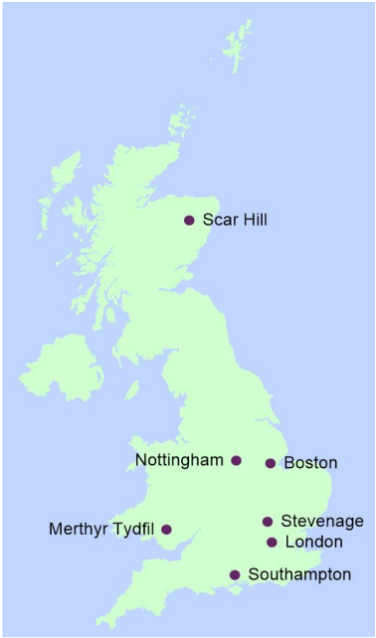
\includegraphics[width=0.4\linewidth]{Figures/Data Pre-Processing/UK_Locations.png}}
        \caption{Measurement locations in the UK and description of topographies \parencite{ofcom2024ml}}
        \label{fig:uk_loc}
    \end{figure}
    \item \textbf{Scarhill:} Mountainous terrain with dense and high vegetation. The terrain rises to the west of the transmitter to heights of greater than 800 m. To the east the ground height falls to approximately 100 m.\parencite{ofcom2024ml}
    \item \textbf{Boston:} Flat terrain with hills rising to the west of the transmitter location. The environment is predominantly open with sparse vegetation and three small towns within the service area of the transmitter.\parencite{ofcom2024ml}

\end{itemize}


The measurements were distance triggered and the data was averaged on export from the receiver
using the Lee method as described in Recommendation ITU-R SM.1708 to remove multi path effects.
The Lee criteria parameters are given in Table 1. It should be noted that for the 5850.00 MHz
measurements, the maximum number of samples within the 40 wavelength distance that could be
collected was 35, limited by the maximum pulse rate available from the CAN Bus interface which
gives a minimum distance interval of 5.8 cm. \parencite{ofcom2019uk}




\section{Schema and Metadata}
This report is based on real-world radio wave propagation measurement data collected from Ofcom's open source (UK's communication regulator company). As stated in the data collection section 3.1, This data consists of high-resolution field measurements collected across various sites within UK (where signal towers are present). Data is collected using a driving vehicle and the tower using one as transmitter and other as receiver. The time and location of both transmitter and receiver is being captured along with the local mean measurement value (which can be used to calculate the signal path loss).

The datasets are consists of seven different locations/sites across UK- \textbf{Boston, London, Merthyr, Nottingham, Scarhill, Southampton and Stevenage} and include frequency bands within sub-6 GHz spectrum \textbf{449 MHz, 915 MHz, 1802 MHz, 2695 MHz, 3602 MHz and 5850 MHz}. Each dataset consists of two sections Metadata \& Raw tables

\subsection{Metadata} 
Each dataset contains metadata, which provides contextual information about the overall measurements such as site name, site's coordinates, frequency, transmitter's coordinates, system noise floor and more. Which enables user to differentiate between the datasets and helps in proper segregation of the records before merging. Below are the description of the important metadata present- 
\begin{itemize}
    \item \textbf{Site name:} Corresponds to a larger area (city) tells about the location of the receiver and transmitter in general.
    \item \textbf{Site latitude and Site longitude (deg):} Site's base coordinate in terms of latitude and longitude in degree.
    \item \textbf{Frequency (MHz):} Frequency at which signal is being transmitted and received to record the strength in Mega Hertz unit.
    \item \textbf{Tx antenna height (m):} Heights of the transmitter antenna height in meters.
    \item \textbf{Rx antenna height (m):} Heights of the receiver antenna height in meters.
    \item \textbf{Adjusted e.i.r.p (dBm):} Calculated as $\left(\text{Amplifier Output} + \text{Antenna Gain}\right) - \text{Cable Loss}$ in terms of decibels referenced to 1 mil-watt.
    \item \textbf{System noise floor (dBm):} Refers to the lowest power level at which receiver can detect and differentiate the signal from noise (also calculated in terms of decibels referenced to 1 mil-watt)
\end{itemize}
    
\subsection{Raw Table} 
Rest of the file contains table with different number of columns as shown below:-
\begin{itemize}
    \item \textbf{Date (dd.mm.yyyy):} Represents the date when a specific data point was recorded.
    \item \textbf{Time (hh:mm:ss):} States the time of the data collection.
    \item \textbf{Rx Latitude (deg)}: Latitude coordinates of the receiver.
    \item \textbf{Rx Longitude (deg)}: Longitude coordinates of the receiver.
    \item \textbf{Local mean measurement (dBm):} Mean Signal Strength measured over a small area.
\end{itemize}

Additionally there are some additional metadata in some of the regions which are not being used in the process as it is not available for rest of the sites. For example - Cable loss, amplifier power, system gain etc.



\section{Data Pre-Processing}

The accuracy of any machine learning technique is totally based on how well a data is processed before it feeds into the model. Processing of data includes - initial cleaning, data reading, post read cleaning, merging of different files (in case required), data type handling, feature transformations, data filtering and creation of any specific metrics that might be required in any analytical analysis before modeling process, specially, when we talk about real world data there are definitely some errors / discrepancies present either due to human error while recording the data or some technical glitch in the process. 

As already stated in the previous sections that data has some discrepancies. This section deals with those discrepancies and explains about changes that has been done on the data to prepare it for modeling purpose.  

Apart from difference in metadata information there are some other issues in the datasets for different sites that can be seen in the pictures below.

\begin{figure}[H]
    \centering
    \fbox{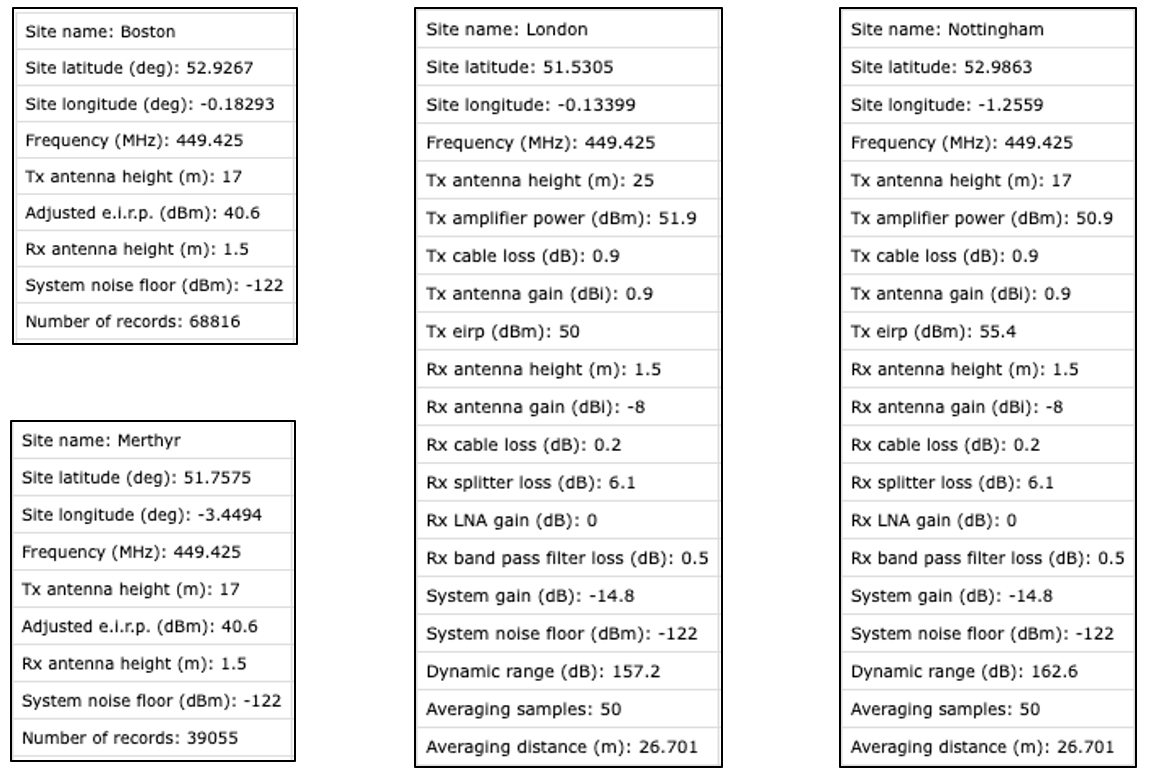
\includegraphics[width=0.8\linewidth]{Figures/Data Pre-Processing/metadata_columns.png}}
    \caption{Metadata values across different datasets}
    \label{fig:meta-data}
\end{figure}


As observed, there are different metadata presents for different sites, another issue in the data is the inconsistency in the column or feature names across different sites and same inconsistency is also present in the measurement table as well. To address these inconsistency and issues in the raw file, the clean up workflow is divided into two stages namely excel based and python based. Detailed information is present below.

\subsection{Excel Based Pre-Processing}
This processing step is for the basic changes that can be done easily and would require some manual interventions. As mentioned there are different metadata present in files for different sites. 
    \begin{enumerate}
        \item Clean the names in the metadata and make all of names similar by renaming the them different in the files and removing the rows that are not required in the processing before loading the data into the python.
        \item Perform the name cleaning process for the data table as well to make sure when you merge the files it does not create additional columns.
    \end{enumerate} 
    
    Make these changes in the excel file itself and try to maintain the consistency across different names and metadata information, which is present in each of the files across different sites and frequency ranges.

\subsection{Python Based Pre-Processing}
This section is an exhaustive exercise including data reading till the data is cleaned and prepared enough to perform any statistical analysis. Once data is pre-cleaned in excel to maintain similar structure and nomenclature. we read the data into python and start with the next step of pre-processing. Below are the detailed information of the steps taken to clean the data and make it analysis ready-

\begin{enumerate}
    \item \textbf{Data Loading:} The datasets were provided in multiple csv format files and is being feed into python. Due to slight structural differences across files, a custom data-reading and cleaning function (\texttt{read\_and\_clean\_file()}) was created, which detects the delimiters in the files, extract the metadata, standardizes some of the column names (to make it easier to read), apply the filters on the signal levels based on the noise threshold as recommended for the bands i.e., filter based on the rule -
    \[\text{Local dBm} > \text{Noise Floor} + 6\,\text{dB}\] 
    
    \textit{*Where \textbf{Local dBm }is the nomenclature used for \textbf{Mean Measurement Value}}
    
    and then merge all the files to create a single dataset. Below is the snippet of the final dataset created-
    \begin{figure}[H]
        \centering
        \fbox{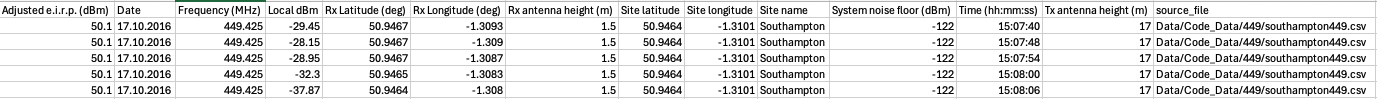
\includegraphics[width=.9\linewidth, height=0.05\textheight]{Figures/Data Pre-Processing/data_read.png}}
        \caption{Combined Dataset After Loading and Filtering}
        \label{fig:data-read}
    \end{figure}

    \item \textbf{Data Cleaning:} It refers to the process to identify and correct (or remove) corrupt or inaccurate records from a dataset and replace or modify or remove the coarse data from that specific dataset. It is an important part of the data processing as raw dataset can include noise or redundant parts that can reduce the quality of the analysis or the productive modeling. There are multiple steps included in data cleaning as mentioned below.

    \begin{enumerate}
        \item \textbf{Trimming Whitespace:} After loading the data all the columns are being checked and trimmed for possible leading or trailing whitespace, to ensure the consistency and to reduce any error due to white spacing.

        \item \textbf{Sanity Check of the data coverage:}Performed the check to estimate the coverage of the data over the various sites and frequencies. It achieved this by collating the dataset into site and frequency groups in order to ascertain coverage and pinpoint areas that did not contain any data.

        \item \textbf{DateTime column creation:}The initial date and time were in two columns. In order to perform any time based filtering and analysis, both the columns (date and time) are combined into one DateTime format. This makes signal transmission trends in time simple to analyze.

        \item \textbf{Removal of original DateTime columns:} Once the column DateTime is created, removed the initial (raw) date and time columns to reduce the dimensionality by removing the redundant columns and clean the table in a more readable form.

        \item \textbf{Handling missing or null values:}All missing, NA and blank cells are replaced with default value 0. This is to ensure that the dataset is all set to be further processed or modeled without errors.
    \end{enumerate}

    This data cleansing process is crucial especially before modeling or analysis as it helps improve the quality and reliability of the dataset by making it accurate and clean. As clean and accurate data is important to prevent errors during model training, improving the accuracy of predictions, and making sure that any findings from the analysis are accurate and meaningful.
\end{enumerate}


\clearpage
 % ------------EDA Section ----------------- 

\chapter{Exploratory Data Analysis}
Exploratory Data Analysis (EDA) is one of the most important step when creating a machine learning model. As this highlights the intricacies in the datasets and helps detect the important features in the table which can easily explain the output variable with minimum error. Also, when the dataset is extremely large such as Ofcom's Radio propagation management data, EDA plays key role in understanding the trends and stability. 

Some of the exploratory data analysis done on the dataset provided are \textbf{Preliminary Validations}, \textbf{Data Distribution}, \textbf{Mean Measurement Value vs. Distance}, \textbf{Spatial Distribution Of Signal Strength}, \textbf{Overall Interpretation}. The detailed description and insights for each of these steps are present in below sections.

\section{Preliminary Validations} 
Once the data is cleaned and pre processed, we perform some basic checks in the start to check the size of data and its quality and analyze whether its a good enough fit for further analysis. For example - checking records at each frequency bands, total number of records per sites, availability of any non-required column (removing which can increase the process time), etc.. Below is a summary of initial processed dataframe.

The below tables gives a brief explanation on the distribution of records in each section. \texttt{Table 4.1} shows clearly that each frequency band has data for all the seven sites, while \texttt{Table 4.2} shows that distribution of records in each frequency site combination.

Based on the insights from \texttt{Table 4.1} we can clearly say that, data is captured for all the frequency and site combinations as each frequency band has all the seven sites mapped against them in the dataset.
 
\begin{table}[H]
    \centering
    \begin{tabular}{|c|c|}
    \hline
    \rowcolor{myblue}
    \textcolor{white}{\textbf{Frequency (MHz)}} & \textcolor{white}{\textbf{\#Sites}} \\
    \hline
    449.425 & 7 \\ \cdashline{1-2}[.4pt/2pt]
    915.95  & 7 \\ \cdashline{1-2}[.4pt/2pt]
    1802.5  & 7 \\ \cdashline{1-2}[.4pt/2pt]
    2695.0  & 7 \\ \cdashline{1-2}[.4pt/2pt]
    3602.5  & 7 \\ \cdashline{1-2}[.4pt/2pt]
    5850.0  & 7 \\ \cdashline{1-2}[.4pt/2pt]
    \hline
    \end{tabular}
    \caption{Available Number of Sites For Each Frequency}
    \label{tab:freq_site}
\end{table}

The second table \texttt{Table 4.2} provides deeper insights into number of records captured after data cleaning and pre-processing. Some of the insights based on the information in table are- 

\begin{itemize}
    \item Number of records varies across site and frequency combinations, showing the difference in data collection intensity.
    \item Some sites such as Boston and Scarhill has consistently higher number of record capture as compared to other sites across different frequencies. While Merthyr and Southampton has lower record capture.
\end{itemize}


\begin{table}[H]
\centering
    % First row: 449.425 and 915.950
    \begin{minipage}[t]{0.45\textwidth}
    \centering
    \captionof{}{Frequency: 449.425 MHz}
    \begin{tabular}{|l|r|}
    \hline
    \rowcolor{myblue}
    \textcolor{white}{\textbf{Site Name}} & \textcolor{white}{\textbf{\#Records}} \\
    \hline
    Boston & 61,248 \\ \cdashline{1-2}[.4pt/2pt]
    London & 26,149 \\ \cdashline{1-2}[.4pt/2pt]
    Merthyr & 21,392 \\ \cdashline{1-2}[.4pt/2pt]
    Nottingham & 45,297 \\ \cdashline{1-2}[.4pt/2pt]
    ScarHill & 60,723 \\ \cdashline{1-2}[.4pt/2pt]
    Southampton & 23,347 \\ \cdashline{1-2}[.4pt/2pt]
    Stevenage & 35,439 \\ 
    \hline
    \end{tabular}
    \end{minipage}
    \hfill
    \begin{minipage}[t]{0.45\textwidth}
    \centering
    \captionof{}{Frequency: 915.95 MHz}
    \begin{tabular}{|l|r|}
    \hline
    \rowcolor{myblue}
    \textcolor{white}{\textbf{Site Name}} & \textcolor{white}{\textbf{\#Records}} \\
    \hline
    Boston & 116,080 \\ \cdashline{1-2}[.4pt/2pt]
    London & 54,402 \\ \cdashline{1-2}[.4pt/2pt]
    Merthyr & 42,725 \\ \cdashline{1-2}[.4pt/2pt]
    Nottingham & 92,970 \\ \cdashline{1-2}[.4pt/2pt]
    ScarHill & 116,268 \\ \cdashline{1-2}[.4pt/2pt]
    Southampton & 53,597 \\ \cdashline{1-2}[.4pt/2pt]
    Stevenage & 71,997 \\ 
    \hline
    \end{tabular}
    \end{minipage}
    
    \vspace{1em}
    
    % Second row: 1802.500 and 2695.000
    \begin{minipage}[t]{0.45\textwidth}
    \centering
    \captionof{}{Frequency: 1802.5 MHz}
    \begin{tabular}{|l|r|}
    \hline
    \rowcolor{myblue}
    \textcolor{white}{\textbf{Site Name}} & \textcolor{white}{\textbf{\#Records}} \\
    \hline
    Boston & 200,700 \\ \cdashline{1-2}[.4pt/2pt]
    London & 56,945 \\ \cdashline{1-2}[.4pt/2pt]
    Merthyr & 72,571 \\ \cdashline{1-2}[.4pt/2pt]
    Nottingham & 144,312 \\ \cdashline{1-2}[.4pt/2pt]
    ScarHill & 116,106 \\ \cdashline{1-2}[.4pt/2pt]
    Southampton & 58,092 \\ \cdashline{1-2}[.4pt/2pt]
    Stevenage & 45,367 \\ 
    \hline
    \end{tabular}
    \end{minipage}
    \hfill
    \begin{minipage}[t]{0.45\textwidth}
    \centering
    \captionof{}{Frequency: 2695.0 MHz}
    \begin{tabular}{|l|r|}
    \hline
    \rowcolor{myblue}
    \textcolor{white}{\textbf{Site Name}} & \textcolor{white}{\textbf{\#Records}} \\
    \hline
    Boston & 240,384 \\ \cdashline{1-2}[.4pt/2pt]
    London & 61,588 \\ \cdashline{1-2}[.4pt/2pt]
    Merthyr & 83,589 \\ \cdashline{1-2}[.4pt/2pt]
    Nottingham & 165,968 \\ \cdashline{1-2}[.4pt/2pt]
    ScarHill & 98,209 \\ \cdashline{1-2}[.4pt/2pt]
    Southampton & 63,942 \\ \cdashline{1-2}[.4pt/2pt]
    Stevenage & 53,853 \\ 
    \hline
    \end{tabular}
    \end{minipage}
    
    \vspace{1em}
    
    % Third row: 3602.500 and 5850.000
    \begin{minipage}[t]{0.45\textwidth}
    \centering
    \captionof{}{Frequency: 3602.5 MHz}
    \begin{tabular}{|l|r|}
    \hline
    \rowcolor{myblue}
    \textcolor{white}{\textbf{Site Name}} & \textcolor{white}{\textbf{\#Records}} \\
    \hline
    Boston & 425,094 \\ \cdashline{1-2}[.4pt/2pt]
    London & 128,340 \\ \cdashline{1-2}[.4pt/2pt]
    Merthyr & 121,184 \\ \cdashline{1-2}[.4pt/2pt]
    Nottingham & 162,004 \\ \cdashline{1-2}[.4pt/2pt]
    ScarHill & 247,693 \\ \cdashline{1-2}[.4pt/2pt]
    Southampton & 104,213 \\ \cdashline{1-2}[.4pt/2pt]
    Stevenage & 94,700 \\
    \hline
    \end{tabular}
    \end{minipage}
    \hfill
    \begin{minipage}[t]{0.45\textwidth}
    \centering
    \captionof{}{Frequency: 5850.0 MHz}
    \begin{tabular}{|l|r|}
    \hline
    \rowcolor{myblue}
    \textcolor{white}{\textbf{Site Name}} & \textcolor{white}{\textbf{\#Records}} \\
    \hline
    Boston & 549,252 \\ \cdashline{1-2}[.4pt/2pt]
    London & 130,849 \\ \cdashline{1-2}[.4pt/2pt]
    Merthyr & 178,484 \\ \cdashline{1-2}[.4pt/2pt]
    Nottingham & 217,394 \\ \cdashline{1-2}[.4pt/2pt]
    ScarHill & 290,660 \\ \cdashline{1-2}[.4pt/2pt]
    Southampton & 128,458 \\ \cdashline{1-2}[.4pt/2pt]
    Stevenage & 105,736 \\
    \hline
\end{tabular}
\end{minipage}
\caption{Total Number of Records Per Site and Frequency Combination}
\end{table}

These insights indicate that whilst the site coverage per frequency is consistent, the records per site is not — an important factor to bear in mind while modeling and analysis as they can cause bias or skew prediction outputs.

The line chart present below compares shows the distribution of samples across sites and frequency bands, revealing both overall site variation and frequency-dependent site variations. It is clearly visible that \textbf{Boston} has the largest number of samples among all frequency bands, while London, Southampton and Stevenage stand out from the rest of the measurements as consistently lower sample groups which is same as that in the \texttt{Table 4.2}. Although the exact number of samples differs between sites between bands, overall trends with number of samples across sites is similar across all frequency bands, indicating relative ordering of sites by number of samples is largely consistent between frequency \texttt{Figure 4.1}

Additionally, we could also see that higher bands (e.g., 3602.5 MHz and 5850 MHz) have more recorded samples in comparison to lower bands such as 449.425 MHz or 915.95 MHz. This implies that the measurement setup or propagation characteristics tend to collect denser data set at higher frequencies, which may be a result of shorter-range signals detected more frequently. 

In summary, these results suggest that, despite variation in absolute number of records across sites, a similar frequency band distribution pattern is maintained indicating strong site-determination over data availability.


\begin{figure}[H]
    \centering
    \fbox{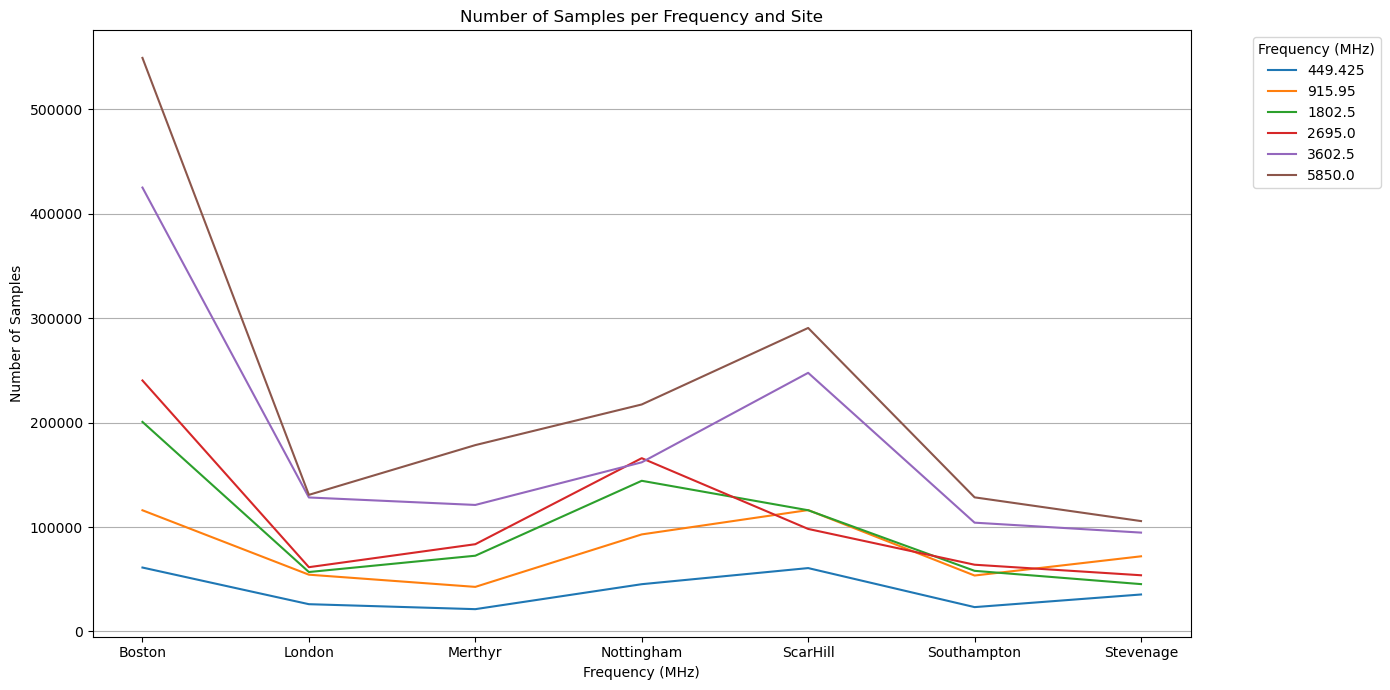
\includegraphics[width=1\linewidth, height = 0.35\textheight]{Figures/EDA/samples_per_freq_site.png}}
    \caption{Total Number of Records Per Site and Frequency Combination}
    \label{fig:data-read}
\end{figure}



\section{Data Distribution} 
Data distribution refers to how values of a particular variable are spread or dispersed across its range. In wireless communication datasets, this often involves examining variables such as signal strength, distance, or frequency. A well-understood distribution helps in identifying trends, outliers, and the overall behavior of the data. For instance, in signal propagation studies, received signal strength (e.g., in dBm) typically shows a negatively skewed distribution due to path loss increasing with distance. Analyzing the distribution allows researchers to detect patterns such as clustering, multi-modal behavior, or long tails, which may be caused by environmental factors, terrain variations, or network configurations \parencite{haykin2005modern}.

\begin{figure}[H]
    \centering
    \fbox{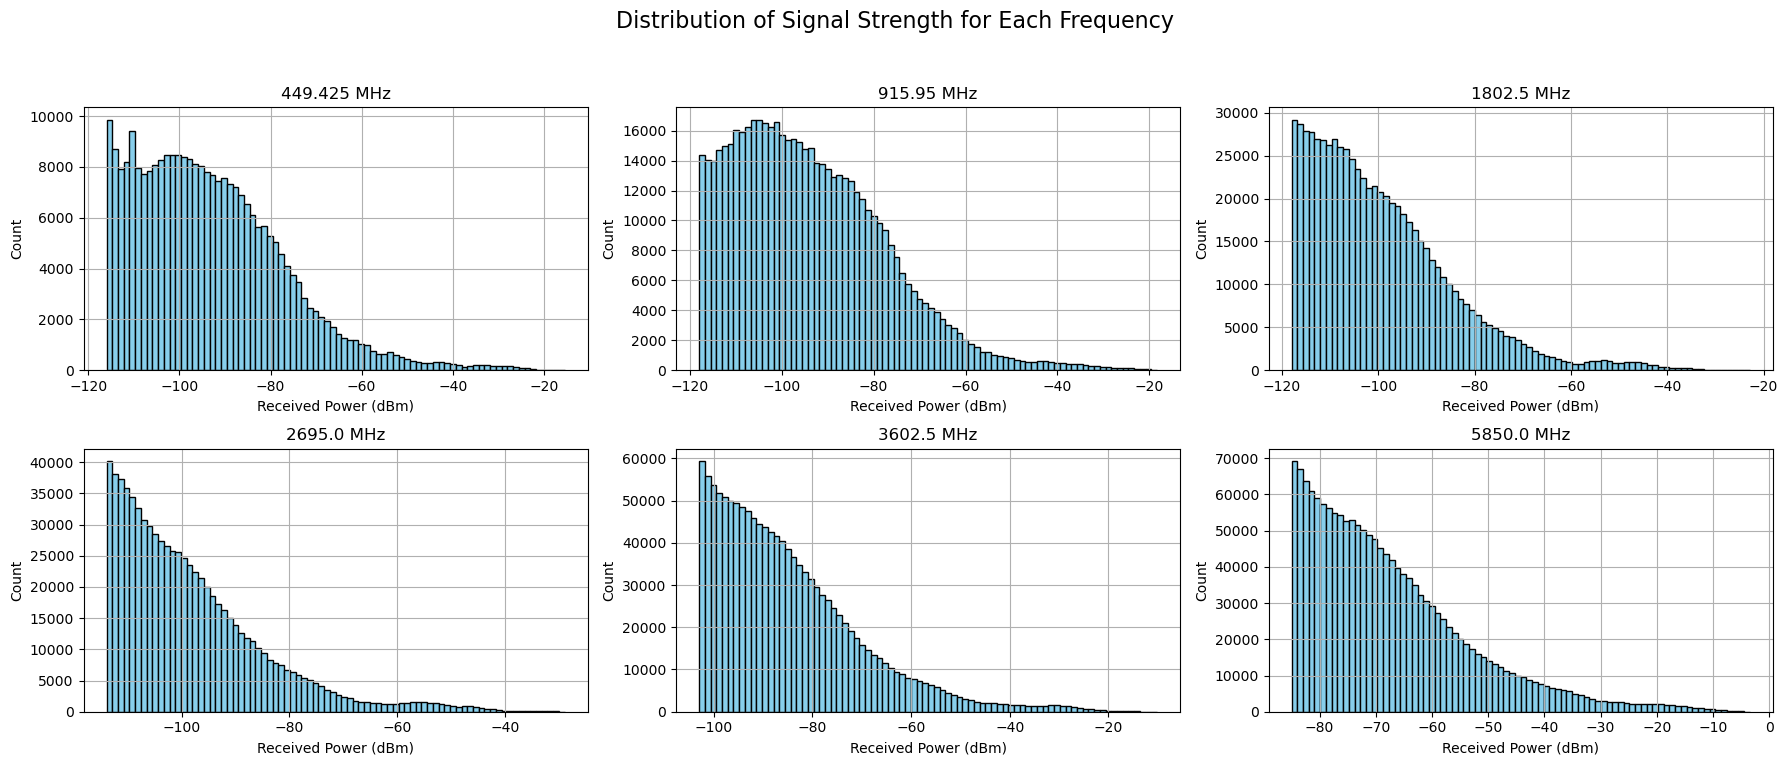
\includegraphics[width=0.9\linewidth, height = 0.3\textheight]{Figures/EDA/Dist_signal_str_freq.png}}
    \caption{Distribution Of Signal Strength by Frequency}
    \label{fig:placeholder}
\end{figure}
In the current dataset and as per the graph above, variables such as \texttt{Local\_dBm} values are concentrated around lower signal strengths, reflecting signal attenuation over distance and obstacles. This pattern aligns with the fundamental radio propagation theory, where power decays logarithmically with distance \parencite{rappaport2002wireless}. Scatter plots and correlation analyses further reinforce this trend, showing a negative correlation between distance and received signal strength. Understanding these distributions is crucial for optimizing network performance, adjusting power levels, and modeling realistic propagation environments \parencite{goldsmith2005wireless}.

\section{Mean Measurement Value vs. Distance:} 
Calculating distance between Tx and Rx and comparing with signal strength, enables us to understand if distance between both the transmitter and receiver is one of the key reasons for increase in signal loss. For that we used the latitude and longitude values of Tx/Rx module and then calculate the distance using \texttt{(geodesic)} function of python. Once the distance is calculated we can check the correlation between the signal path loss (local mean measurement) value and the distance factor. 

Based on the correlation plot shown below \texttt{Figure 4.3}, as the distance between transmitter and receiver increases the mean measurement value (signal power) decreases. This is inline with the \textbf{path loss theory}. At short distance the signal strength is much stronger (almost between 0 to -20dBm), as the distance increases the signal drops to close to -120 dBm. Also, between 10 to 30 kms the signal strength decreases sharply could be because of non line of sight (NLOS) factors like topography, multiple fadings etc. 


\begin{figure}[H]
    \centering
    \fbox{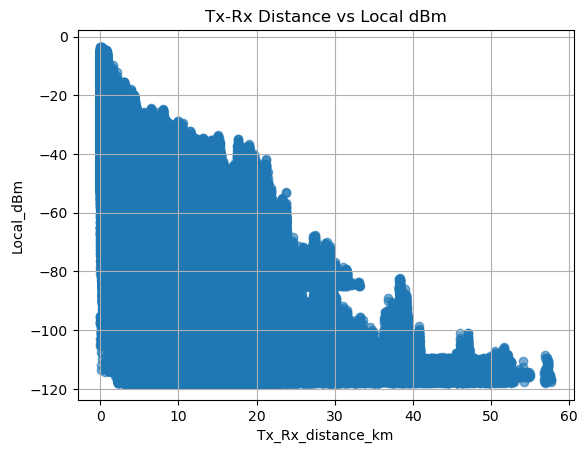
\includegraphics[width=.9\linewidth, height = 0.3\textheight]{Figures/EDA/Corr_Dist_dBm.png}}
    \caption{Relationship Between Transmitter-Receiver Distance \& Received Signal Strength (Local dBm)}
    \label{fig:data-read}
\end{figure}

You can also see specific bands of power levels at certain distances in the scatter. As an example, frequency band, terrain type, or even power control level. It might also represent limits of hardware sensitivity in the receiver.


\section{Spatial Distribution of Signal Strength} 
\texttt{Figure 6} to \texttt{Figure 12} shows the spatial distribution of the received signal strength for all the sites across all the available frequencies from 449.5 to 5850 MHz. This can help us discover some important patterns in terms of signal distribution and its strength across different demography.

\subsection{Coverage Pattern Based on Frequency} 
We can easily observe the variation in signal strength with change in frequency. Generally, lower frequency bands (e.g., 449.425MHz) tends to show wider coverage and have stronger signal strength over large area coverage due to less signal path loss, whereas higher frequency bands (e.g., 5850MHz) show attenuation faster and hence covers very small area.

\subsection{Signal Distribution across Demography}
These charts help recover areas with low and high signal strength across different sites. Areas with higher signal strength (shown in green/yellow color) indicates receiver and transmitter are in close proximity to each other or having line of sight propagation. While, areas with lower signal strength (shown in blue/purple color)  indicates possibility of interference, some obstruction or propagation issues.

\subsection{Effect of Environment on Signal Strength} 
As we know the surroundings play important role in signal strength, we can easily make assumption of the type of environment based on the pattern. For example, any consistent drop-off pattern or any sharp boundary in plot might suggest that the coverage is of an urban area or having terrain features which is obstructing the signal propagation dropping the signal strength while recording it.

\subsection{Comparison of Performance Across Different Frequency Bands}  
Looking at all the six frequencies side by side allows us to compare how each frequency perform in a certain region. This is useful when deciding which one to prioritize either coverage or strength capacity.
      
\begin{figure}[H]
    \centering
    \fbox{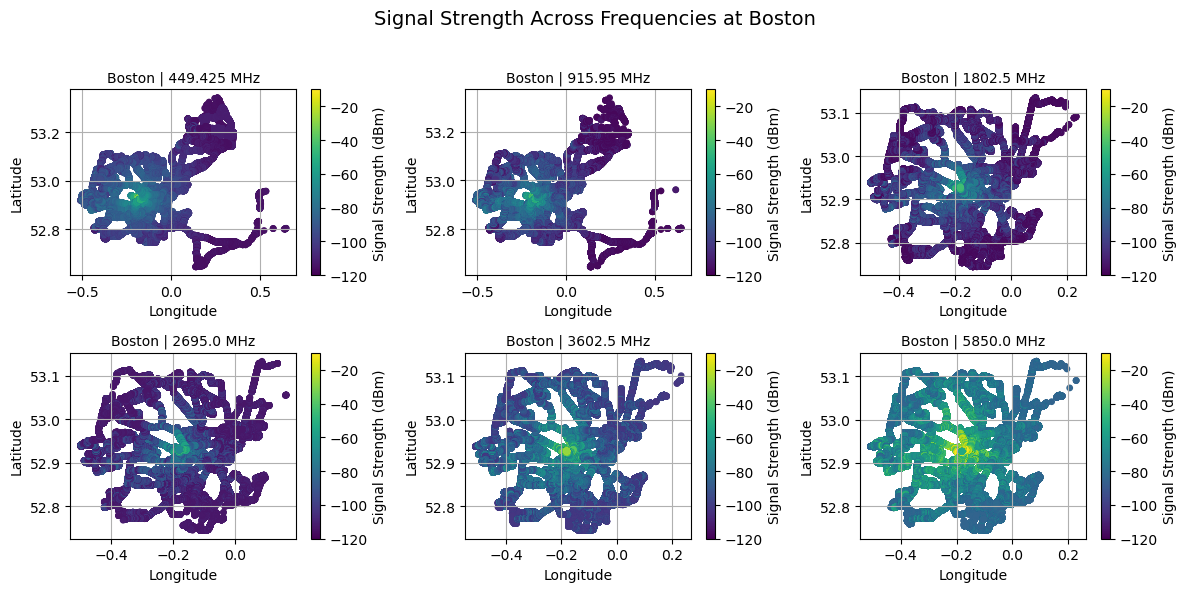
\includegraphics[width=.9\linewidth, height = 0.3\textheight]{Figures/EDA/Boston_Signal_str.png}}
    \caption{Signal Strength Across Frequencies at Boston}
    \label{fig:data-read}
\end{figure}
\texttt{Figure 4.4} shows the distribution across different frequencies in \textbf{Boston} region. As per expectation, lower frequency bands shows higher coverage in terms of area while higher frequencies exhibits more localized signal footprints.  

\begin{figure}[H]
    \centering
    \fbox{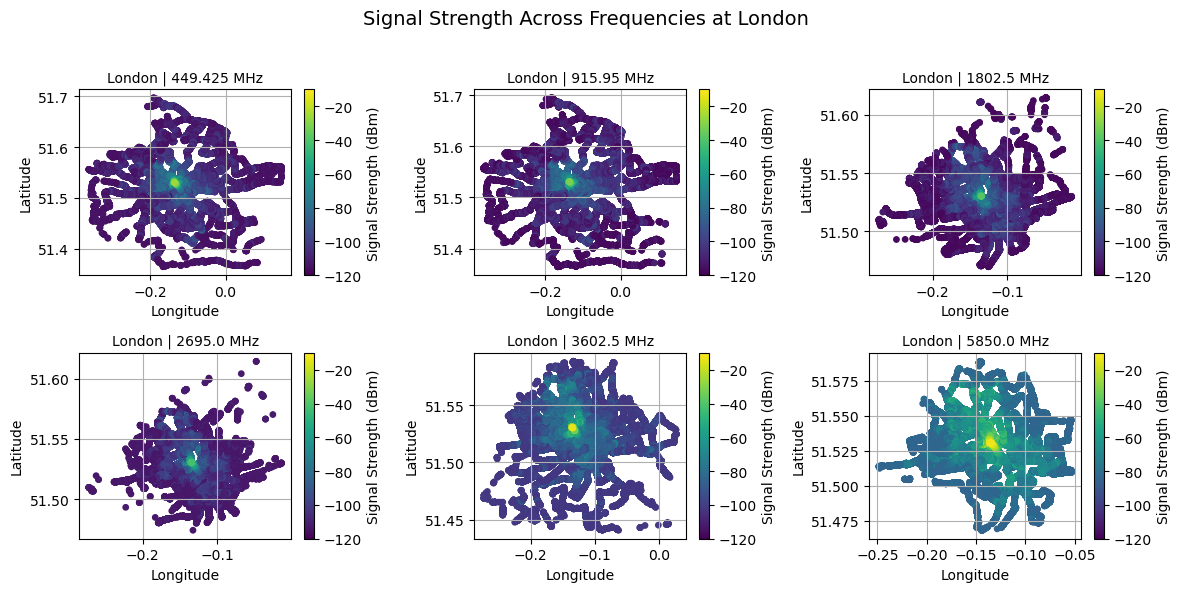
\includegraphics[width=.9\linewidth, height = 0.3\textheight]{Figures/EDA/London_signal_str.png}}
    \caption{Signal Strength Across Frequencies at London}
    \label{fig:data-read}
\end{figure}
\texttt{Figure 4.5} shows the distribution across different frequencies in \textbf{London} region. Similar to Boston higher frequencies in London as well shows low coverage, but the coverage is even lower suggesting more signal loss due to interference. Also, we know London has the most number of high rise buildings in UK compared to all the other regions hence proves the hypothesis.

\begin{figure}[H]
    \centering
    \fbox{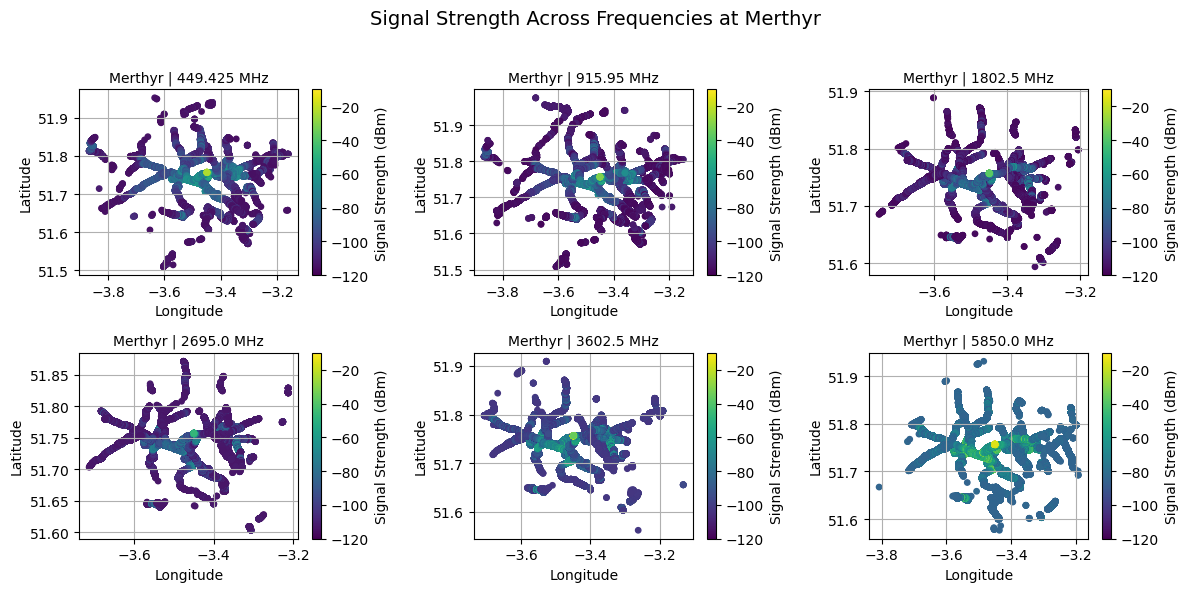
\includegraphics[width=.9\linewidth, height = 0.3\textheight]{Figures/EDA/Merthyr_signal_str.png}}
    \caption{Signal Strength Across Frequencies at Merthyr}
    \label{fig:data-read}
\end{figure}
 The Merthyr area signal distribution over frequencies is shown in \texttt{Figure 4.6}. These patterns are very different from the simple NLOS (non line of sight) behaviour for Stevenage, which implies strong environmental impacts here, as you might expect in terms of obstruction from the terrain and possible even structural density, leading to more shadowing and NLOS effects. Although lower frequencies (449.425 MHz, 915.95 MHz) still have larger footprints, their spread is not as uniform as elsewhere due to propagation.


\begin{figure}[H]
    \centering
    \fbox{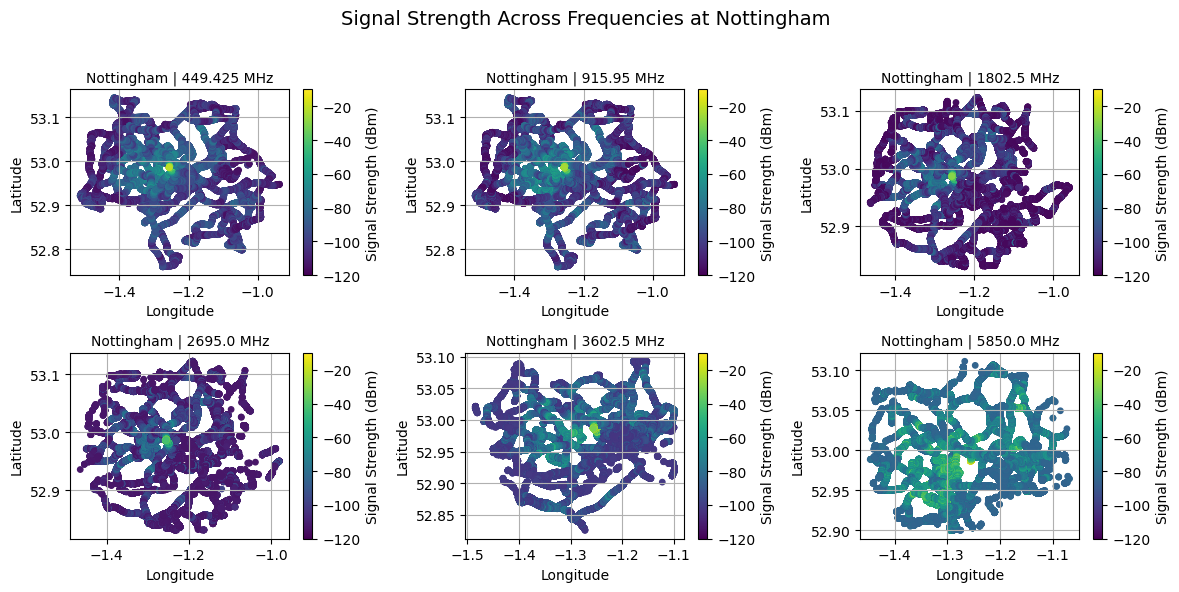
\includegraphics[width=.9\linewidth, height = 0.3\textheight]{Figures/EDA/Nottingham_Signal_Str.png}}
    \caption{Signal Strength Across Frequencies at Nottingham}
    \label{fig:data-read}
\end{figure}
\texttt{Figure 4.7} shows the distribution across different frequencies in \textbf{Nottingham} region. As per expectation, lower frequency bands shows higher geographic coverage with stronger penetration across different. Also, higher frequency bands shows higher coverage with strong signal in small region, highlighting simple trade off, as lower frequency bands are more effective for wider range  while higher frequencies exhibits more localized signal footprints suitable for capacity oriented deployment.

\begin{figure}[H]
    \centering
    \fbox{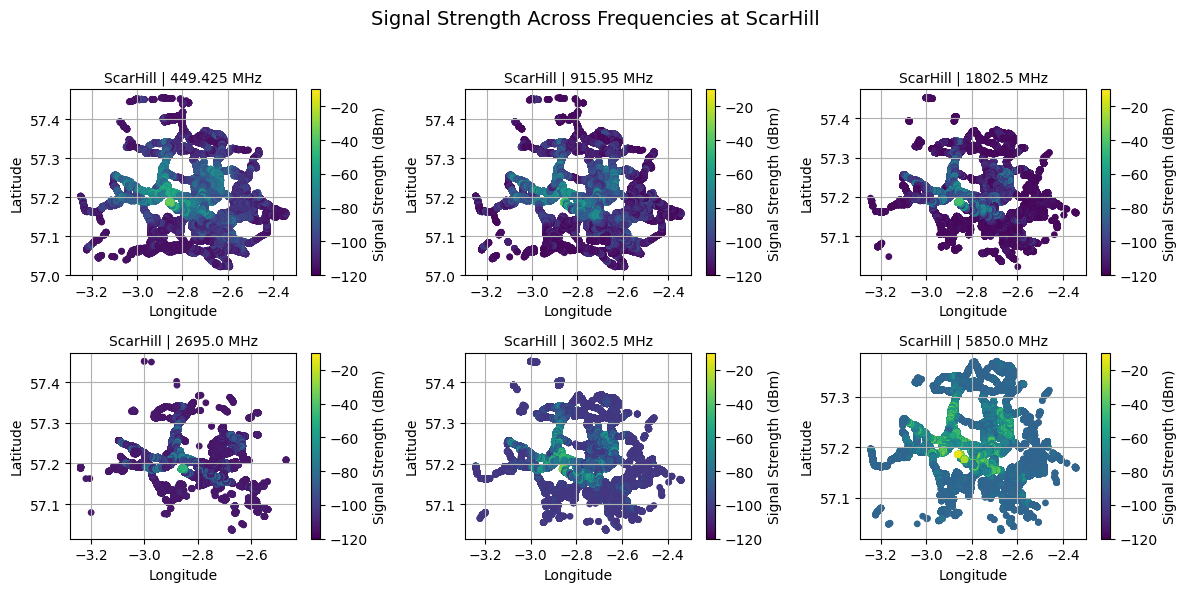
\includegraphics[width=.9\linewidth, height = 0.3\textheight]{Figures/EDA/ScarHill_Signal_Str.png}}
    \caption{Signal Strength Across Frequencies at ScarHill}
    \label{fig:data-read}
\end{figure}
\texttt{Figure 4.8} shows the distribution across different frequencies in \textbf{ScarHill} region.Similar to Nottingham, lower frequency shows higher coverage over large area and higher frequency shows more scattered and localized footprint with visible signal fluctuations due to terrains or environmental issues. 


\begin{figure}[H]
    \centering
    \fbox{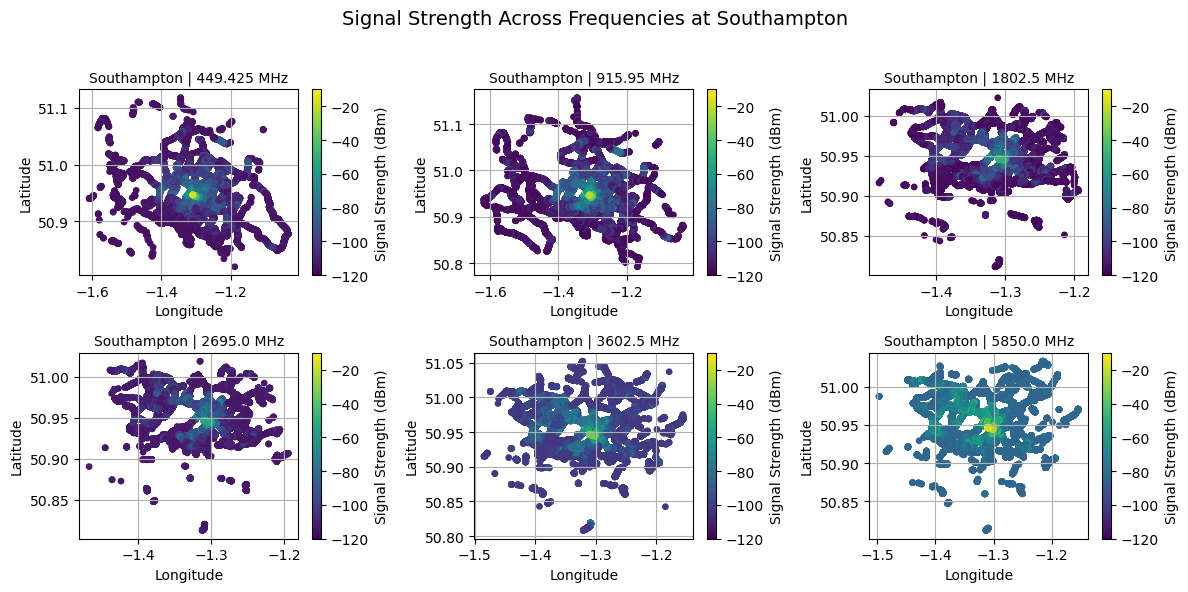
\includegraphics[width=.9\linewidth, height = 0.3\textheight]{Figures/EDA/Southampton_Signal_Str.png}}
    \caption{Signal Strength Across Frequencies at Southampton}
    \label{fig:data-read}
\end{figure}
\texttt{Figure 4.9} shows the distribution across different frequencies in \textbf{Southampton} region. Similar to Nottingham, lower frequency bands shows higher coverage in terms of area while higher frequencies exhibits more localized signal footprints with strong signal over small area. This suggests that the topography of ScarHill may enhance the differential propagation effects function of frequency making higher bands more prone to fragmentation in coverage than in Nottingham.


\begin{figure}[H]
    \centering
    \fbox{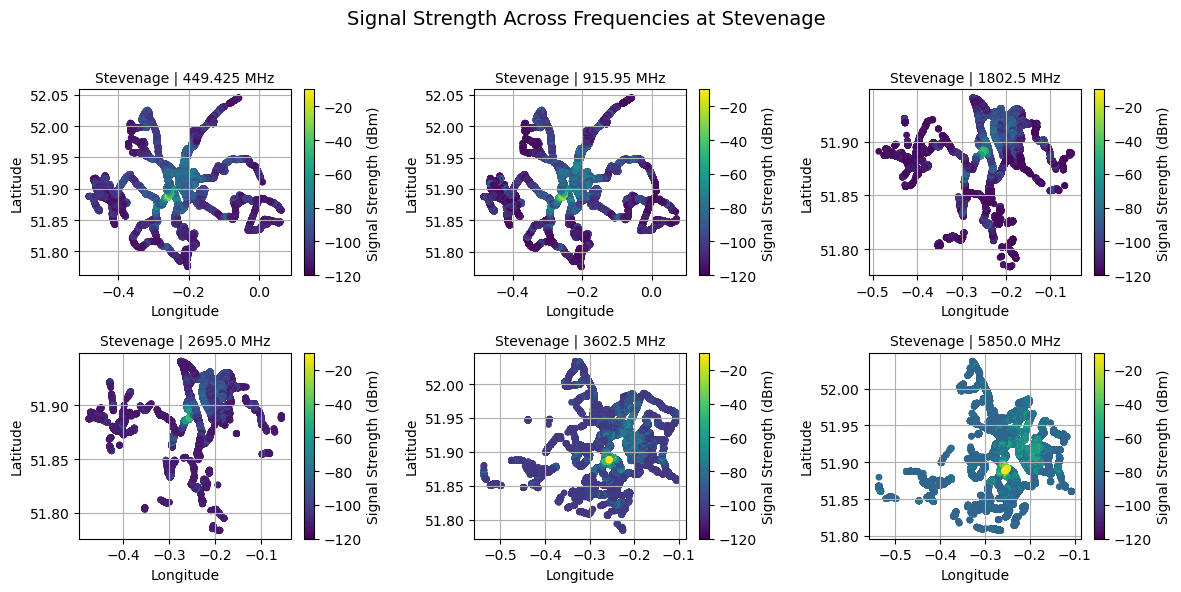
\includegraphics[width=.9\linewidth, height = 0.3\textheight]{Figures/EDA/Stevenage_Signal_Str.png}}
    \caption{Signal Strength Across Frequencies at Stevenage}
    \label{fig:data-read}
\end{figure}
\texttt{Figure 4.10} shows the distribution across different frequencies in \textbf{Stevenage}. As per expectation, lower frequencies (e.g 449.425 MHz, 915.95 MHz) achieve wider, more uniform geographic coverage, spreading our signal footprint across the area. On the lower end of the spectrum, you will get a more cohesive coverage pattern, while on the higher end, you get what is essentially spot coverage with the signal being concentrated in a small area.Stevenage, crucially, demonstrates fairly good signal continuity through all the bands indicating that the urban form and geography is conducive to relatively uniform propagation.


\section{Overall Interpretation}
The above EDA (Exploratory Data Analysis) clearly shows that the frequency, demography and the distance of the signal wave propagation influences the strength of the signal and effect the path loss. Additionally, based on the scatter plots, it can be clearly seen that the change frequency from lower to higher band effect the coverage with lower frequency having higher coverage and it gradually decreases as frequency increases i.e., 
    \[\text{Frequency} \propto \frac{1}{\text{Coverage}}\]
Also, it can be written as- 
    \[\text{Frequency} \propto {\text{Attenuation}}\]

 In additional to frequency, the spatial patterns of signal strength across different sites shows the impact of the environment and topography of a certain site, including the density of architectural stuctures (buildings) in urban areas (For e.g., London) and possibility of available terrain induced shadowing (For e.g., Merthyr).

Furthermore, based on the correlation analysis, it can be observed that a strong negative correlation between the distance  between transmitter and receiver and signal strength. Which confirms that the distance is an important feature causing the signal path loss.
\[\text{Distance b\\w Transmitter \& Receiver } \propto {\text{Signal Path Loss}}\]

As per data is concerned, based on the tables it is clear that, there is enough number of records to train-validate and test a machine or deep learning model which can incorporate all these features, patterns and their relationships to finally access/predict the signal strength (\texttt{mean measurement value}) under different conditions.



 % ------------Model Selection Section -----------------   
\clearpage
\chapter{Methodology}

\section{Introduction To Regression}

Regression analysis is a fundamental statistical technique used to model the relationship between a dependent variable and one or more independent variables \parencite{freedman2009statistical, montgomery2021introduction}. It is widely employed to describe, predict, and infer causal effects in empirical research. In its simplest form, \textit{simple linear regression} assumes a linear relationship between the outcome $Y$ and a single predictor $X$, represented as:
\[
Y = \alpha + \beta X + \varepsilon,
\]
where $\alpha$ denotes the intercept, $\beta$ the slope coefficient, and $\varepsilon$ the random error term \parencite{seber2003linear}. Estimation is typically performed via the \textit{ordinary least squares} (OLS) method, which minimizes the sum of squared residuals. For multiple predictors, the model generalizes to:
\[
Y_i = \beta_0 + \beta_1 X_{1i} + \beta_2 X_{2i} + \cdots + \beta_p X_{pi} + \varepsilon_i,
\]
or in matrix notation:
\[
\mathbf{y} = \mathbf{X}\boldsymbol{\beta} + \boldsymbol{\varepsilon},
\]
with the OLS solution given by:
\[
\hat{\boldsymbol{\beta}} = (\mathbf{X}^T \mathbf{X})^{-1} \mathbf{X}^T \mathbf{y}.
\]
Regression assumes linearity, independence, and homoscedasticity of errors, making it highly interpretable but sometimes restrictive in practice. In contrast, non-parametric ensemble methods such as Random Forests \parencite{breiman2001randomforests} relax these assumptions, capturing nonlinear relationships and complex interactions by averaging over multiple decision trees:
\[
\hat{f}_{RF}(X) = \frac{1}{B} \sum_{b=1}^B T_b(X),
\]
where $T_b(X)$ is the prediction from the $b$-th tree and $B$ is the number of trees in the ensemble. While Random Forests often achieve higher predictive accuracy in complex datasets, regression remains essential for its interpretability and explanatory power \parencite{strobl2009introduction, ishwaran2007variable}.



\section{Model Selection \& Designs}
Based on the insights gathered from the previous section (Exploratory Data Analysis) we can use that for model selection. Also, as per the correlation between distance and signal strength insights and relationship of various factors like frequency, site location, topography etc. we will be taking a step wise approach for a machine learning model which can help us compare the results at different levels and helps us show the impact of different features in predicting the signal strength. The machine learning model we will train will be a \texttt{Random Forest Regression Model}, which is well suited for a grouped and nested data like Ofcom's. Below mentioned are the models will be training for this use case and how they can help us generalizing the results balancing coverage and capacity.

Random forest model is chosen for its robustness over a linear regression model for predicting signal strength. In addition to robustness, it is scalable and is suitable for a non-linear relationship between features which is an important factor in our case. This model also takes care of outliers and noises in case there are some present in the data. 
\begin{itemize}
    \item It works well in case of more data available. As it is a decision tree based model each tree is trained on a different bootstrapped subset of the data, having a higher volume of samples ensures that trees capture more diverse patterns and structures within the dataset. This diversity results in a more robust and generalized ensemble model, reducing the risk of overfitting and variance in predictions. As a result, Random Forest performance typically improves as more data becomes available \parencite{breiman2001randomforests}.

    \item Due to its ensemble feature Random Forest is robust to overfitting as it averages multiple decision trees on the different bootstrapped data samples. Training on single decision tree might result into overfitting but since it run on multiple decision trees it generally does not overfit.

    \item It also handles missing and correlated data very well. For example- if some of the values in the data is missing or if some of the features are correlated (e.g., distance and signal strength), it will still be reliable to run this model. Additionally, it does not require any strict assumptions as linear regression does.

    \item Most importantly it works well with spatial data like latitude, longitude and Distance as they benefits from the way random forest split data into train and test enable it to capture the local patterns.
\end{itemize}

\section{Random Forest Models}
Random Forest (RF) is a statistical learning theory that uses the bootstrap resampling method to extract multiple samples from the original sample. Each bootstrap sample is used to build a decision tree model,and then multiple decision trees are combined to make predictions. The final prediction result is obtained through voting \parencite{zhang2018aa_pathloss}.

Random Forest Regressor (RFR) is an ensemble regression model composed of many decision tree regression models 
$\{ h(X, \Theta_k), \; k = 1, 2, \ldots \}$, 
where the parameter sets $\{ \Theta_k \}$ are independent and identically distributed random vectors. Random forests for regression are formed by growing trees depending on a random vector
such that the tree predictor h(x, ) takes on numerical values as opposed to class labels.
The output values are numerical and we assume that the training set is independently drawn
from the distribution of the random vector Y, X. The mean-squared generalization error for
any numerical predictor h(x) is, \parencite{breiman2001randomforests}

\[
E_{X,Y} \left( Y - h(X) \right)^2 
\]

Below is the diagram (flow chart) shows working of a random Forest Model in \texttt{Figure 5.1}.

\begin{figure}[h]
    \centering
    \resizebox{\textwidth}{!}{%
    \begin{tikzpicture}[node distance=1cm, every node/.style={font=\small}]
    
    % Node style
    \tikzstyle{block} = [rectangle, draw, minimum height=1.2cm, minimum width=2cm, align=center]
    \tikzstyle{arrow} = [->, thick]
    
    % Nodes
    \node (D) [block] {Dataset $D$};
    \node (rand) [block, right=of D, text width=3.2cm] {Randomization \\ Create random vector $\Theta_k$};
    \node (d1) [block, right=of rand, yshift=1cm] {Sample $D_1$};
    \node (d2) [block, right=of rand] {Sample $D_2$};
    \node (d3) [block, right=of rand, yshift=-1cm] {Sample $D_k$};
    
    \node (trees) [block, right=4.5cm of rand, text width=3.5cm, minimum height=3.5cm] {Trained Decision Trees};
    
    \node (out1) [block, right=of trees, yshift=1.5cm, text width=3.5cm] {Tree 1 \\ Regression Output};
    \node (out2) [block, right=of trees, text width=3.5cm] {Tree 2 \\ Regression Output};
    \node (out3) [block, right=of trees, yshift=-1.5cm, text width=3.5cm] {Tree $k$ \\ Regression Output};
    
    \node (final) [block, right=of out2, xshift=3cm, text width=4.2cm] {Final Prediction \\ (Averaged Output)};
    
    % Arrows
    \draw [arrow] (D) -- (rand);
    \draw [arrow] (rand) -- (d1.west);
    \draw [arrow] (rand) -- (d2.west);
    \draw [arrow] (rand) -- (d3.west);
    
    \draw [arrow] (d1.east) -- (trees.west |- d1.east);
    \draw [arrow] (d2.east) -- (trees.west |- d2.east);
    \draw [arrow] (d3.east) -- (trees.west |- d3.east);
    
    \draw [arrow] (trees.east |- out1.west) -- (out1.west);
    \draw [arrow] (trees.east |- out2.west) -- (out2.west);
    \draw [arrow] (trees.east |- out3.west) -- (out3.west);
    
    \draw [arrow] (out1.east) -- (final.west);
    \draw [arrow] (out2.east) -- (final.west);
    \draw [arrow] (out3.east) -- (final.west);
    
    \end{tikzpicture}
    }
    \caption{Architecture of Random Forest Regressor (RFR)}
\end{figure}

\subsection{Metrics for Evaluating the Performance Model}
Calculating metrics for evaluation is needed to find out how much of a prediction error a model creates. The path loss values obtained from the model prediction will be calculated together with the measured data (actual path loss values). The difference between the measured value and the path loss value predicted by the model is used to calculate. Error metrics such as MAPE and RMSE are used in this study to evaluate the path loss prediction models \parencite{sotiroudis2019neural}, \parencite{moraitis2020machine}. The equations for MAPE and RMSE can be expressed as in (1) and (2).
\[
\text{MAPE} = \frac{1}{N} \sum_{i=1}^{N} \left| \frac{PL_{\text{actual},i} - PL_{\text{predicted},i}}{PL_{\text{actual},i}} \right| \times 100
\tag{1}
\]

\[
\text{RMSE} = \sqrt{ \frac{1}{N} \sum_{i=1}^{N} \left( PL_{\text{actual},i} - PL_{\text{predicted},i} \right)^2 }
\tag{2}
\]

\textit{where PL stands for Path Loss. But for our use case we will measure Mean Measurement Value (Signal Strength)}


\subsection{Different Levels (granularity) of Models}
Once the machine learning model is selected, the next step is to decide what should be the level of insight we need from the model results, as this will help us deciding and grouping the data with certain features. For us looking at various levels empowers us in decision making at different hierarchical levels. For this report, we will be training this model at - 

\begin{enumerate}
    \item \textbf{Frequency Level:} The dataset contains different features and at different granularity. For example - Location ( latitude, longitude, site), Frequency, etc., Training models at Frequency helps explaining how a specific frequency's behavior is different from others in similar or in broad ranges irrespective of any location constraints with different topographies. This can enable deciding which frequency will be better for a specific use case. 
\end{enumerate}

\begin{enumerate}
    \item \textbf{Site \& Frequency Level:} Using Site as an additional feature in the model helps differentiating the predictions based on a specific topography or architectural differences in different sites. This can show the the behavior of frequencies in various different conditions. 
\end{enumerate}

\subsection{Model 1: Random Forest Model at Frequency Level}

To check the performance of the Random Forest model across different frequencies present, separated the data for each frequency and trained and validated the model for each one of them separately (validation set are shown in \textcolor{dodgerblue}{blue} color, test set are shown in \textcolor{darkgreen}{green} color). \texttt{Figure 5.2} to \texttt{Figure 5.7} shows the test and validation results from the trained and tested model. Plots are comparing the actual and measured values of Local dBM (mean measured values) for both the test and the validation datasets. When observed the plots it is clear that each plot has a \textcolor{red}{red dotted} reference line which is inclined at 45\textdegree, showing the accuracy in the prediction of the model.When observed across all the frequencies, the prediction exhibits a strong linear relationship with the actual measured values, indicating that the Random Forest Model is capturing the non-linear relationship in radio wave propagation loss with higher accuracy.

\begin{figure}[H]
    \centering
    \fbox{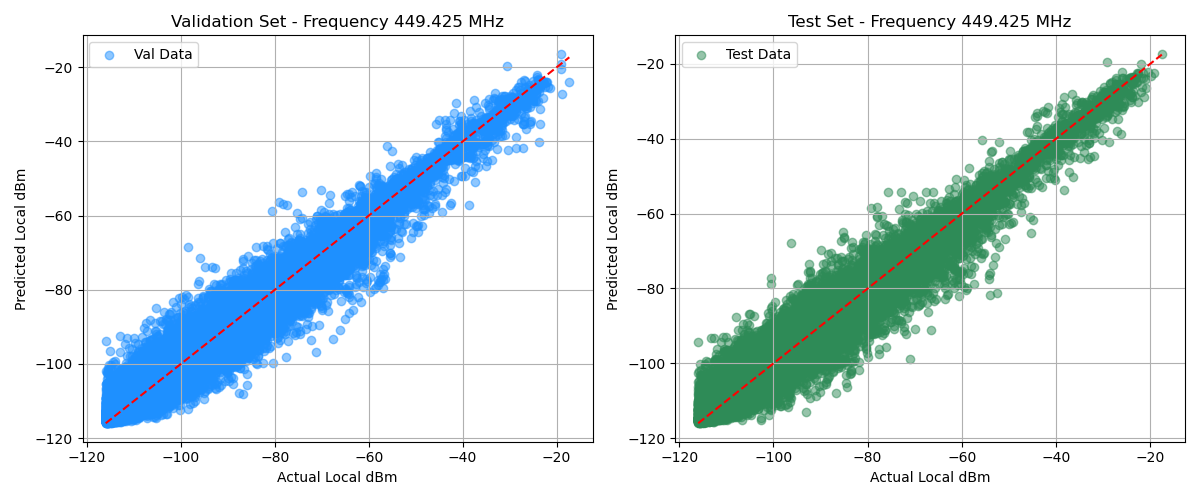
\includegraphics[width=.8\linewidth, height = 0.18\textheight]{Figures/Methodology/RF_F_Level/val_test_side_by_side_freq_449.425.png}}
    \caption{Test \& Validation Results at Frequency 449.425 MHz}
    \label{fig:data-read}
\end{figure}

\begin{figure}[H]
    \centering
    \fbox{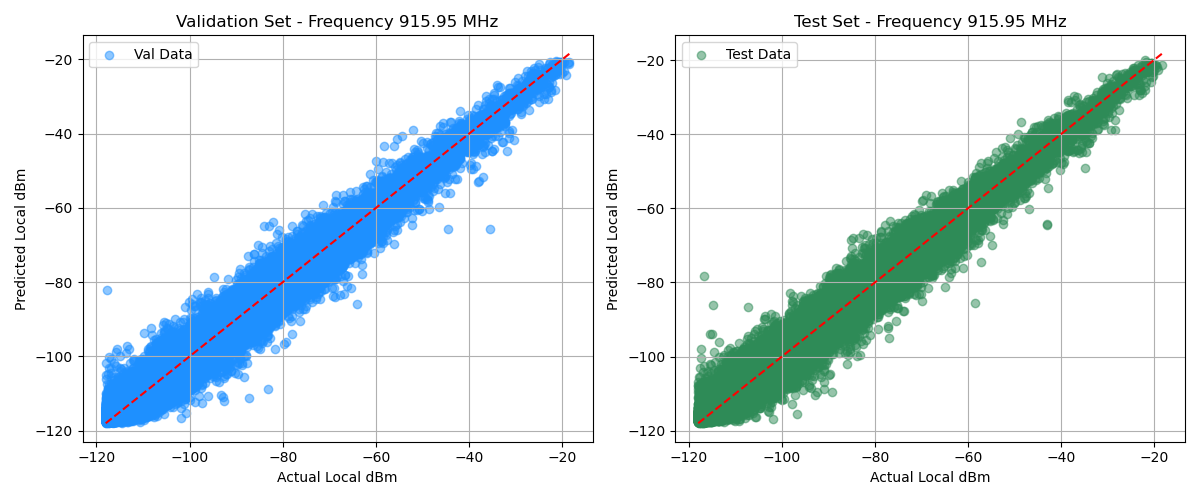
\includegraphics[width=.8\linewidth, height = 0.18\textheight]{Figures/Methodology/RF_F_Level/val_test_side_by_side_freq_915.95.png}}
    \caption{Test \& Validation Results at Frequency 915.95 MHz}
    \label{fig:data-read}
\end{figure}



\begin{figure}[H]
    \centering
    \fbox{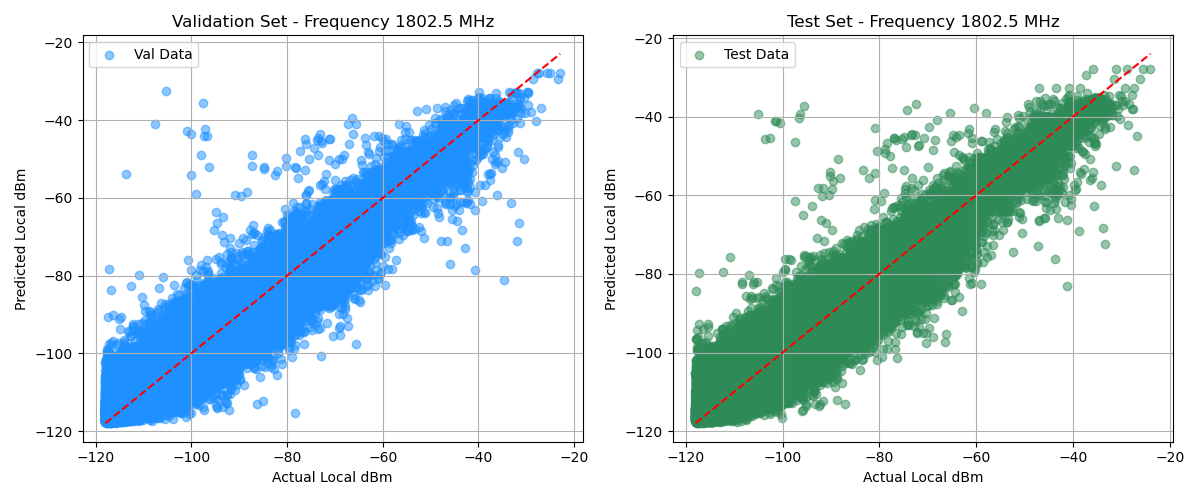
\includegraphics[width=.8\linewidth, height = 0.18\textheight]{Figures/Methodology/RF_F_Level/val_test_side_by_side_freq_1802.5.png}}
    \caption{Test \& Validation Results at Frequency 1802.5 MHz}
    \label{fig:data-read}
\end{figure}

\begin{figure}[H]
    \centering
    \fbox{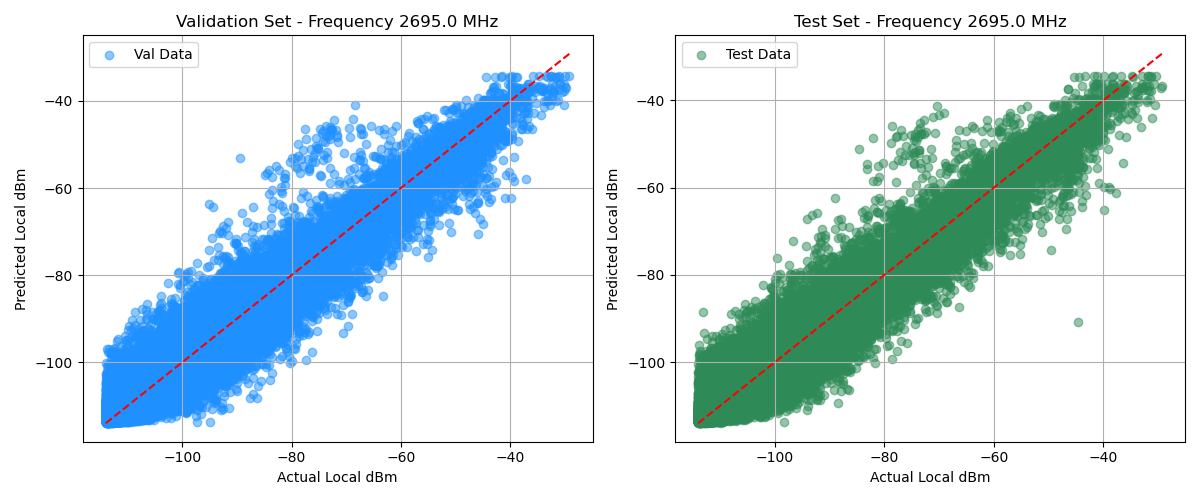
\includegraphics[width=.8\linewidth, height = 0.18\textheight]{Figures/Methodology/RF_F_Level/val_test_side_by_side_freq_2695.0.png}}
    \caption{Test \& Validation Results at Frequency 2695.0 MHz}
    \label{fig:data-read}
\end{figure}

\begin{figure}[H]
    \centering
    \fbox{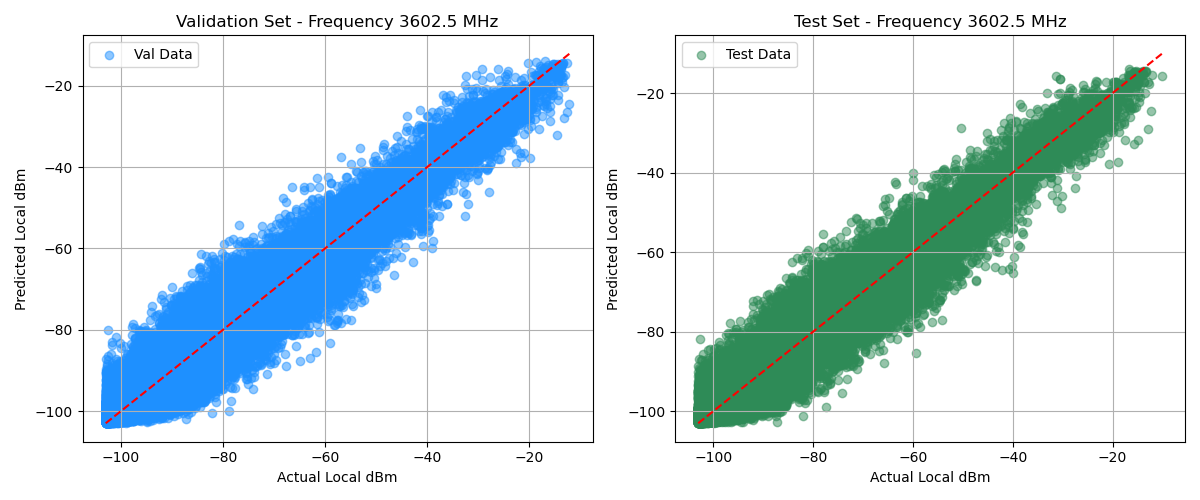
\includegraphics[width=.8\linewidth, height = 0.18\textheight]{Figures/Methodology/RF_F_Level/val_test_side_by_side_freq_3602.5.png}}
    \caption{Test \& Validation Results at Frequency 3602.5 MHz}
    \label{fig:data-read}
\end{figure}

\begin{figure}[H]
    \centering
    \fbox{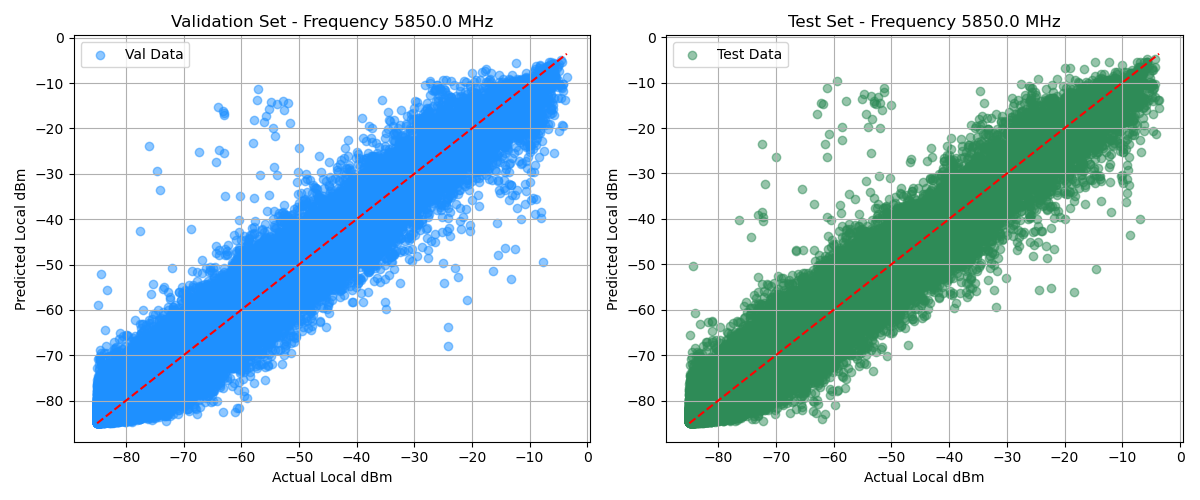
\includegraphics[width=.8\linewidth, height = 0.18\textheight]{Figures/Methodology/RF_F_Level/val_test_side_by_side_freq_5850.0.png}}
    \caption{Test \& Validation Results at Frequency 5850.0 MHz}
    \label{fig:data-read}
\end{figure}

\texttt{Table 5.1} summaries the model's performance metrics Mean Squared Error (MSE), Root Mean Squared Error (RMSE) \& the coefficient of the determination (R$^2$) values for all the frequency bands comparing the metrics for both the test and validation sets. As per the table, the performance remains consistent across the frequencies with R$^2$ ranging between 95\% to 98\%, denoting that the trained model is able to explain more than 95\% of the variance in the data and able to predict well on the test set with out showing any evidence of overfitting. Additionally, low RMSE value (ranging between 2.5 - 3.2) highlights the robustness of the model in minimizing the error prediction.


\begin{table}[h]
    \centering
    \begin{tabular}{|c|c|c|c|c|c|c|c|}
        \hline
        \rowcolor{myblue}
        \textcolor{white}{\textbf{Frequency (MHz)}} & \textcolor{white}{\textbf{Val MSE}}   & \textcolor{white}{\textbf{Val RMSE}} &\textcolor{white}{\textbf{ Val R²}}    & \textcolor{white}{\textbf{Test MSE}} & \textcolor{white}{\textbf{Test RMSE}} & \textcolor{white}{\textbf{Test R²}} \\ \hline
        449.425        & 6.35  & 2.52 & 0.98  & 6.55 & 2.56  & 0.98  \\ \cdashline{1-7}[.4pt/2pt]
        915.950        & 8.10  & 2.85 & 0.97  & 8.09 & 2.84  & 0.97 \\  \cdashline{1-7}[.4pt/2pt]
        1802.500       & 9.73  & 3.12 & 0.95  & 9.70 & 3.11  & 0.95  \\  \cdashline{1-7}[.4pt/2pt]
        2695.000       & 8.82  & 2.97 & 0.95  & 8.81 & 2.97  & 0.95 \\  \cdashline{1-7}[.4pt/2pt]
        3602.500       & 8.54  & 2.92 & 0.96  & 8.37 & 2.89  & 0.96  \\  \cdashline{1-7}[.4pt/2pt]
        5850.000       & 7.90  & 2.81 & 0.96  & 8.01 & 2.83  & 0.96  \\ \hline
    \end{tabular}
    \caption{Model Performance Results Combined For All the Frequencies}
    \label{tab:frequency_stats}
\end{table}

The model results suggests that the model is able to handle lower frequencies bands (449 MHz and 915 MHZ) better than the higher frequency bands with lowest RMSE and highest R$^2$ for band 449.5 MHz. This might be because lower frequency travel more effectively without getting disrupted by any obstacles in the environment or any external signal reflections. Whereas, the model shows higher error in higher frequency bands aligning with the fact that higher frequency bands are sensitive to the environment.

The shown analysis helps understand the behavior of frequency bands irrespective of any location constraints. Though there are some limitations to this analysis listed below- 

\begin{enumerate}
    \item This model does not talk about the effect of location on a specific frequency band and how change in topography can change the model result.
    \item There are some outliers and its not easy to detect any specific reasoning for the cause of the outliers in the data, whether it is specific to a certain frequency or due to a specific location topography. Which will be covered in the next section, where the model is trained at site and frequency level.
\end{enumerate}



\subsection{Model 2: Random Forest Model at Site \& Frequency Level}

In addition to the frequency level model, the Random Forest model is also being trained at Site \& Frequency level to understand the behavior of a frequency band and predict the signal path loss when trained for a specific location. By doing this, allows model to take into consideration the differences in the environment in which the radio wave is propagating, for example population density, topography, clutters which can be very different in different sites.

The test and validation sets are shown in different figures including all the different frequency bands for a specific site. Same as in the previous section the validation sets are in \textcolor{dodgerblue}{blue} and test sets are in \textcolor{darkgreen}{green} colored plots. \texttt{Figure 5.8} to \texttt{Figure 5.21} in pairs of two is combination of these test and validation sets for a specific site, showing the model performance by comparing actual vs measured of the mean measurement values. From looking at bird eye view the model performance seems accurate with some very minor errors. Which is good enough to explain the prediction of path loss.

\begin{figure}[H]
    \centering
    \fbox{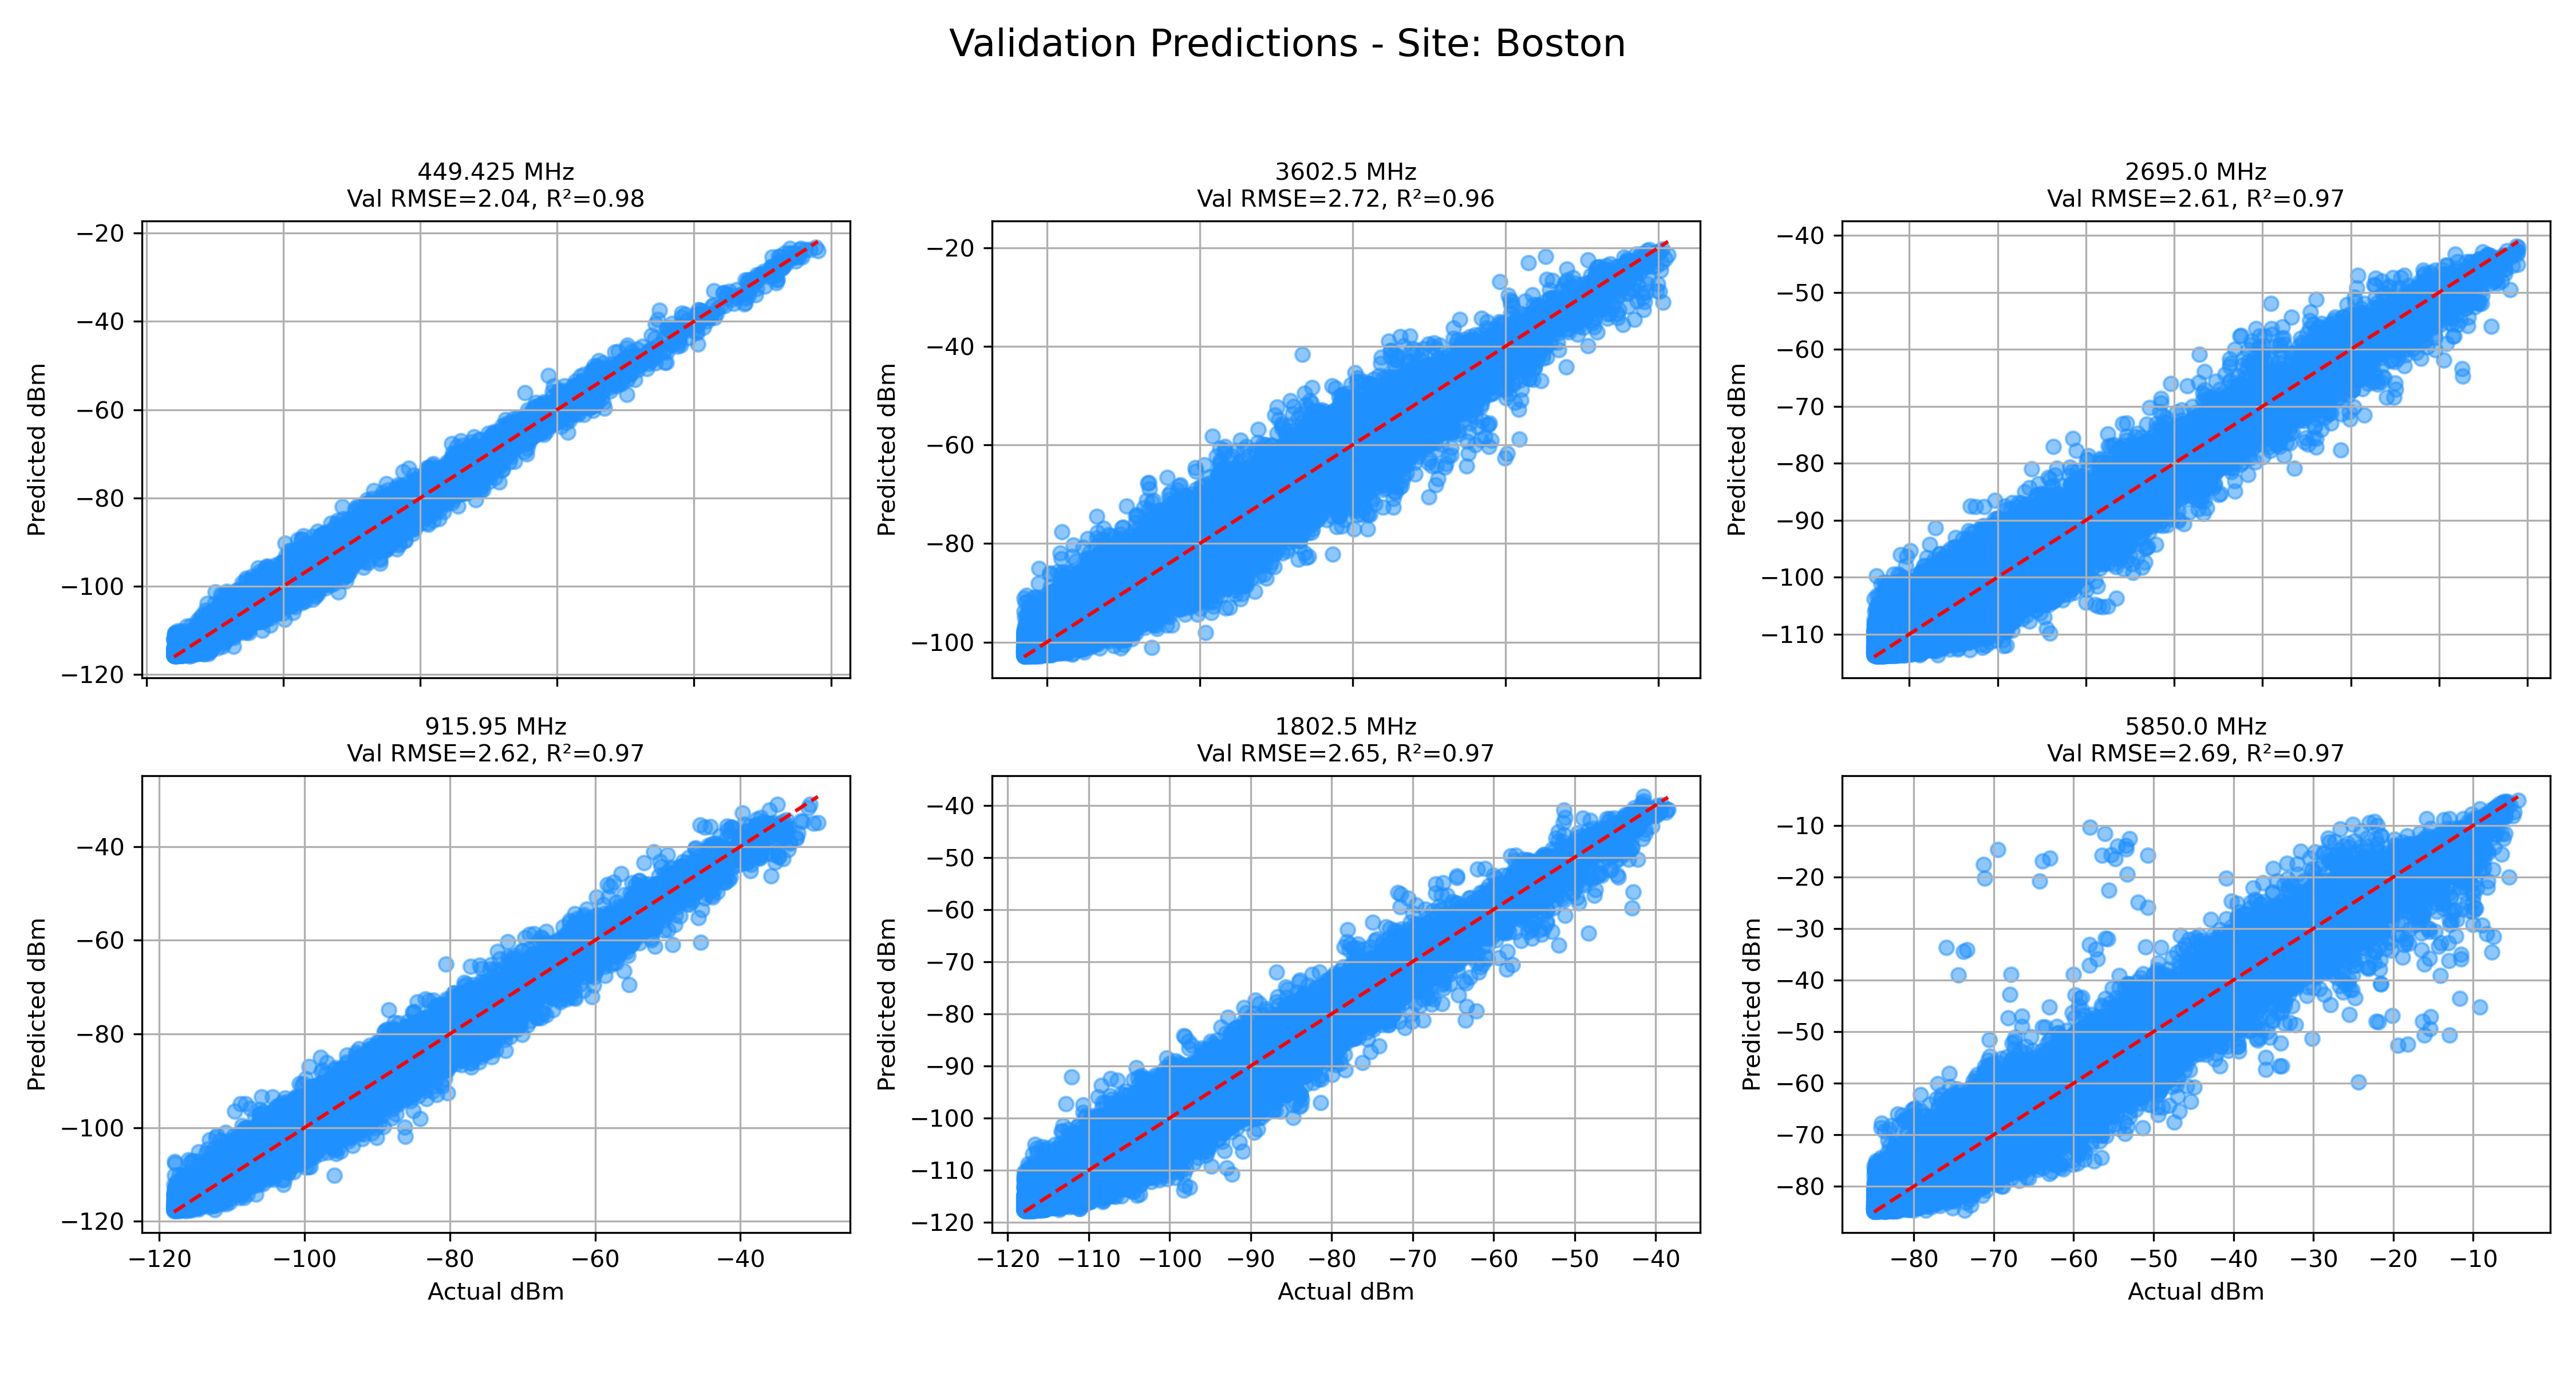
\includegraphics[width=.9\linewidth, height = 0.25\textheight]{Figures/Methodology/RF_F_S_Level/Boston_val.png}}
    \caption{Validation Results Boston}
    \label{fig:data-read}
\end{figure}

\begin{figure}[H]
    \centering
    \fbox{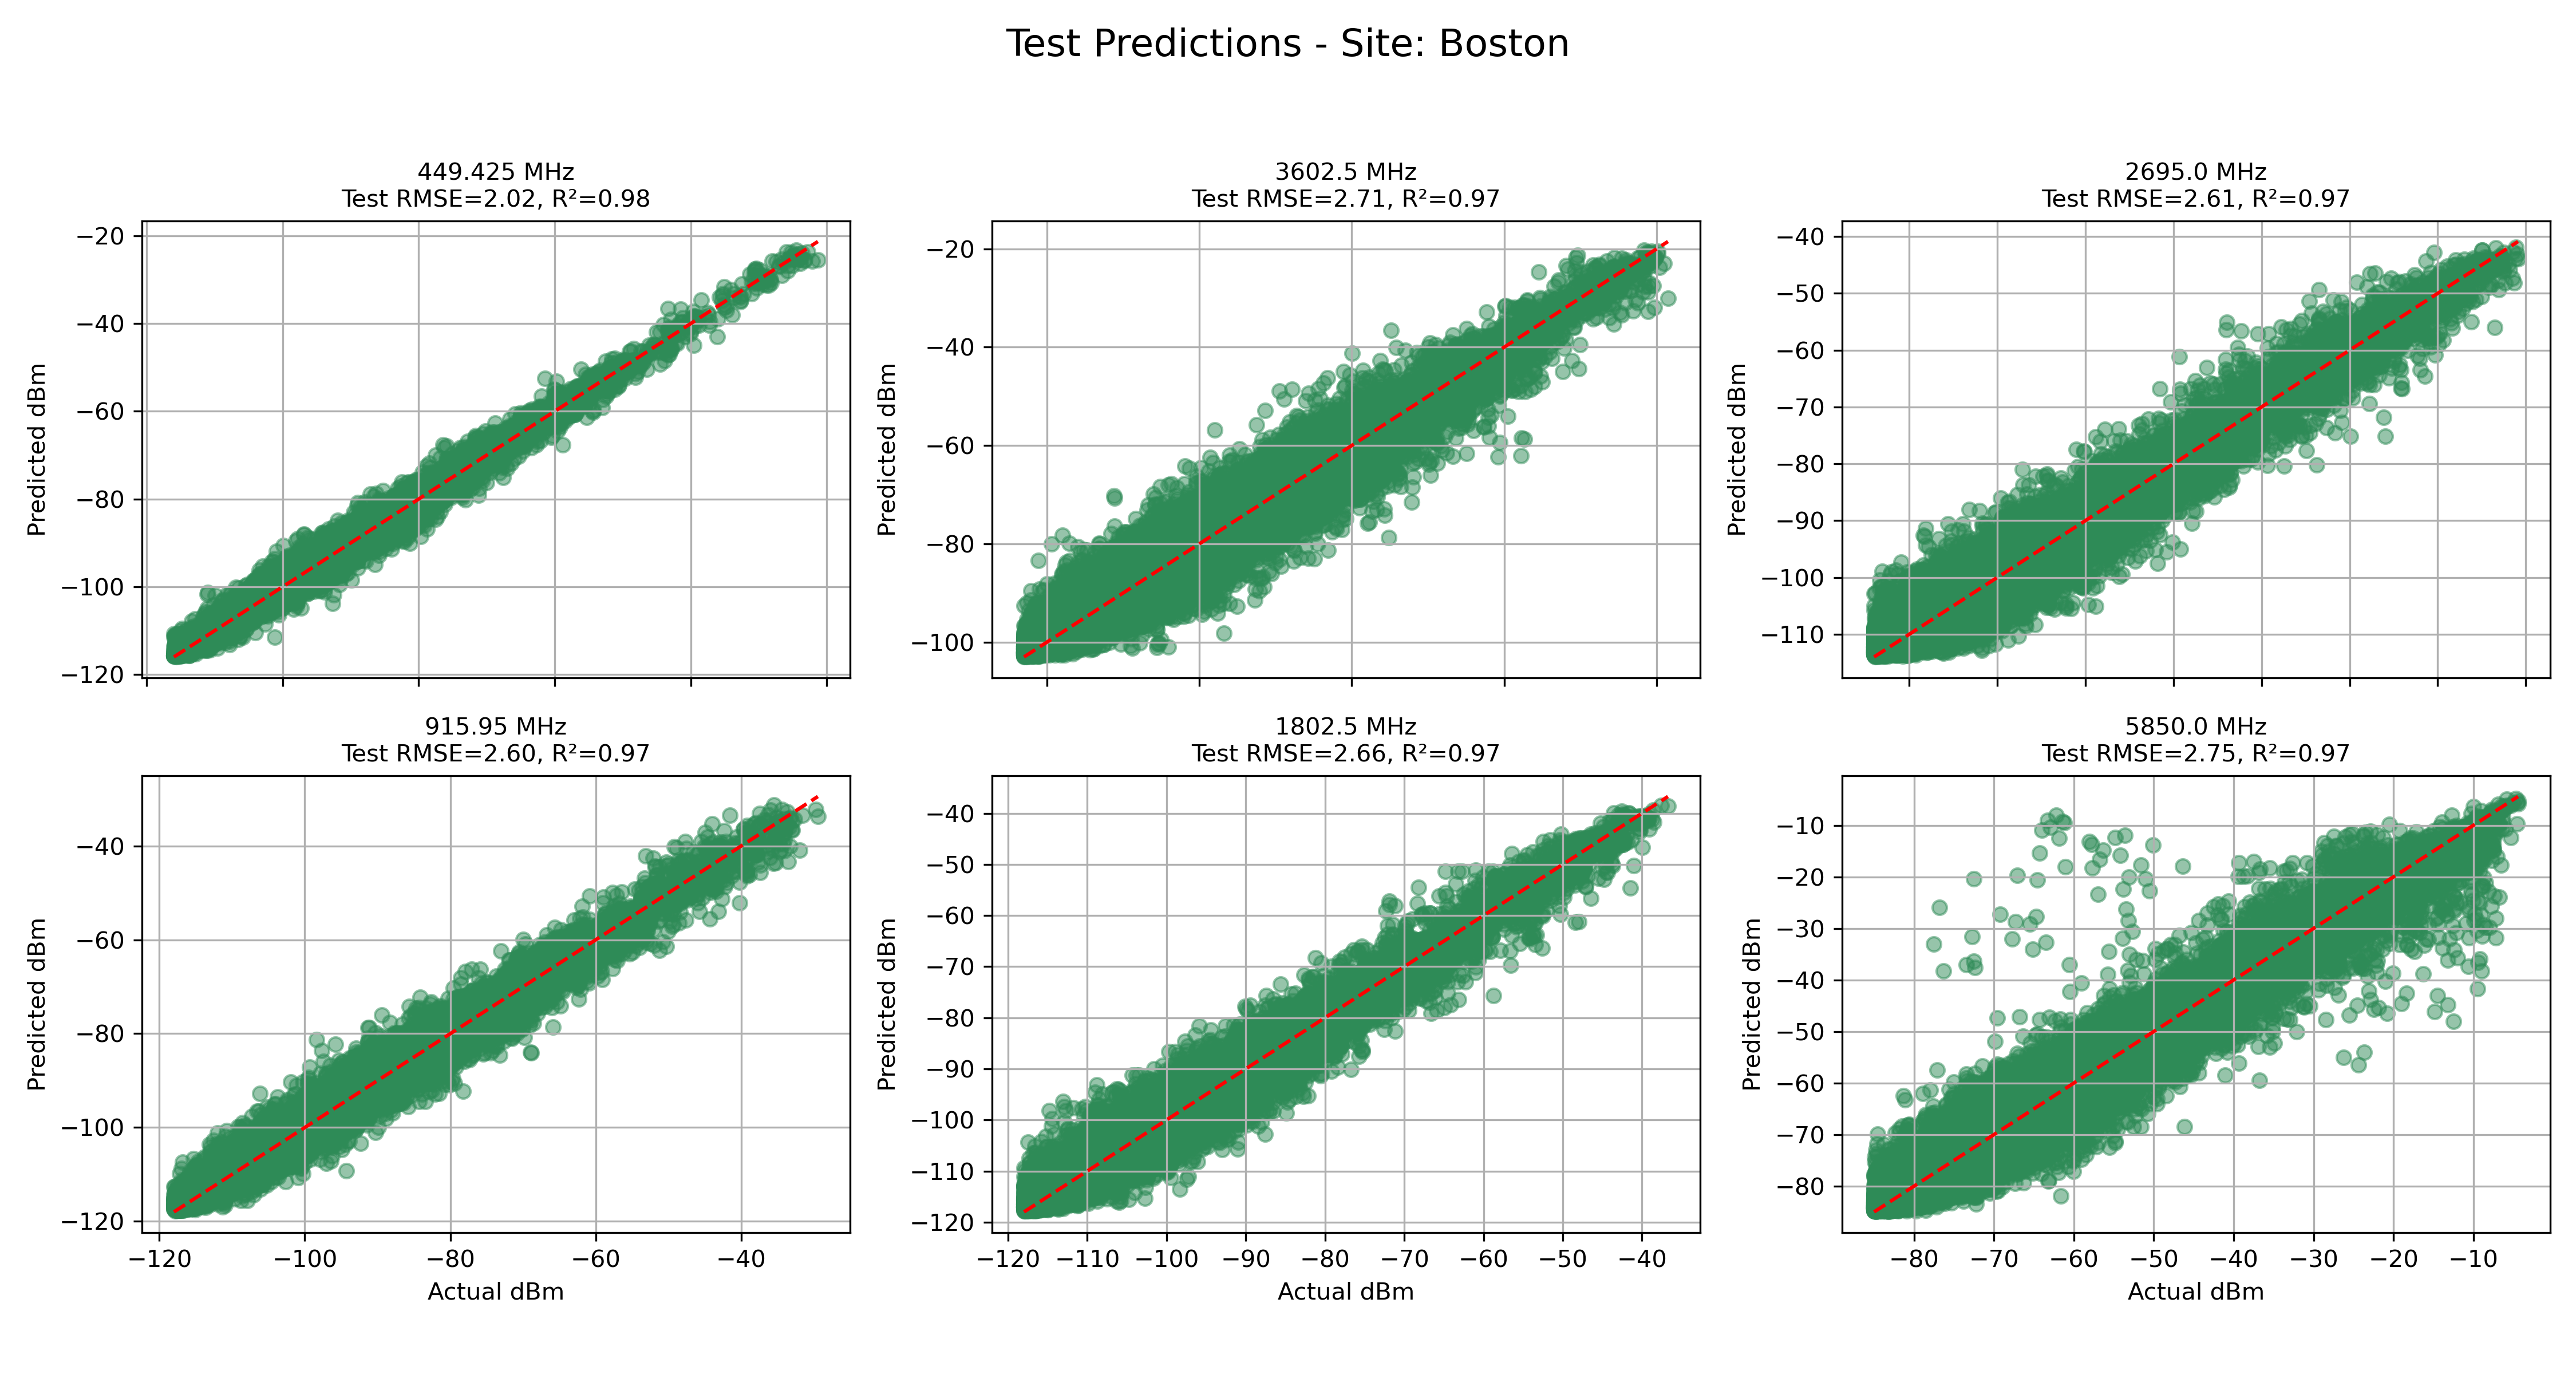
\includegraphics[width=.9\linewidth, height = 0.25\textheight]{Figures/Methodology/RF_F_S_Level/Boston_test.png}}
    \caption{Test Results Boston}
    \label{fig:data-read}
\end{figure}

\begin{table}[h]
    \centering
    \begin{tabular}{|c|c|c|c|c|c|}
        \hline
        \rowcolor{myblue}
        \textcolor{white}{\textbf{Frequency (MHz)}} & 
        \textcolor{white}{\textbf{Val RMSE}} & 
        \textcolor{white}{\textbf{Val R²}} & 
        \textcolor{white}{\textbf{Test RMSE}} & 
        \textcolor{white}{\textbf{Test R²}} & 
        \textcolor{white}{\textbf{Num Samples}} \\ \hline
        449.425        & 2.04 & 0.98 & 2.02 & 0.98 & 61,248  \\ \cdashline{1-6}[.4pt/2pt]
        915.950        & 2.62 & 0.97 & 2.60 & 0.97 & 116,080 \\ \cdashline{1-6}[.4pt/2pt]
        1802.500       & 2.65 & 0.97 & 2.66 & 0.97 & 200,700 \\ \cdashline{1-6}[.4pt/2pt]
        2695.000       & 2.61 & 0.97 & 2.61 & 0.97 & 240,384 \\ \cdashline{1-6}[.4pt/2pt]
        3602.500       & 2.72 & 0.96 & 2.71 & 0.97 & 425,094 \\ \cdashline{1-6}[.4pt/2pt]
        5850.000       & 2.69 & 0.97 & 2.75 & 0.97 & 549,252 \\ \hline
    \end{tabular}
    \caption{Model Performance Results Boston}
    \label{tab:frequency_stats}
\end{table}

\begin{itemize}
    \item \textbf{Observation:} \texttt{Figure 5.8}, \texttt{Figure 5.9} and \texttt{Table 5.2} are the model result for site Boston.
    \begin{itemize}
        \item  When compared the test and validation sets the performance seems very similar on both the sets, confirming that the model generalizes well.  
        \item slightly higher deviation can be observed at higher frequency bands, along with some outliers at highest frequency.
    \end{itemize}

\end{itemize}



\begin{figure}[H]
    \centering
    \fbox{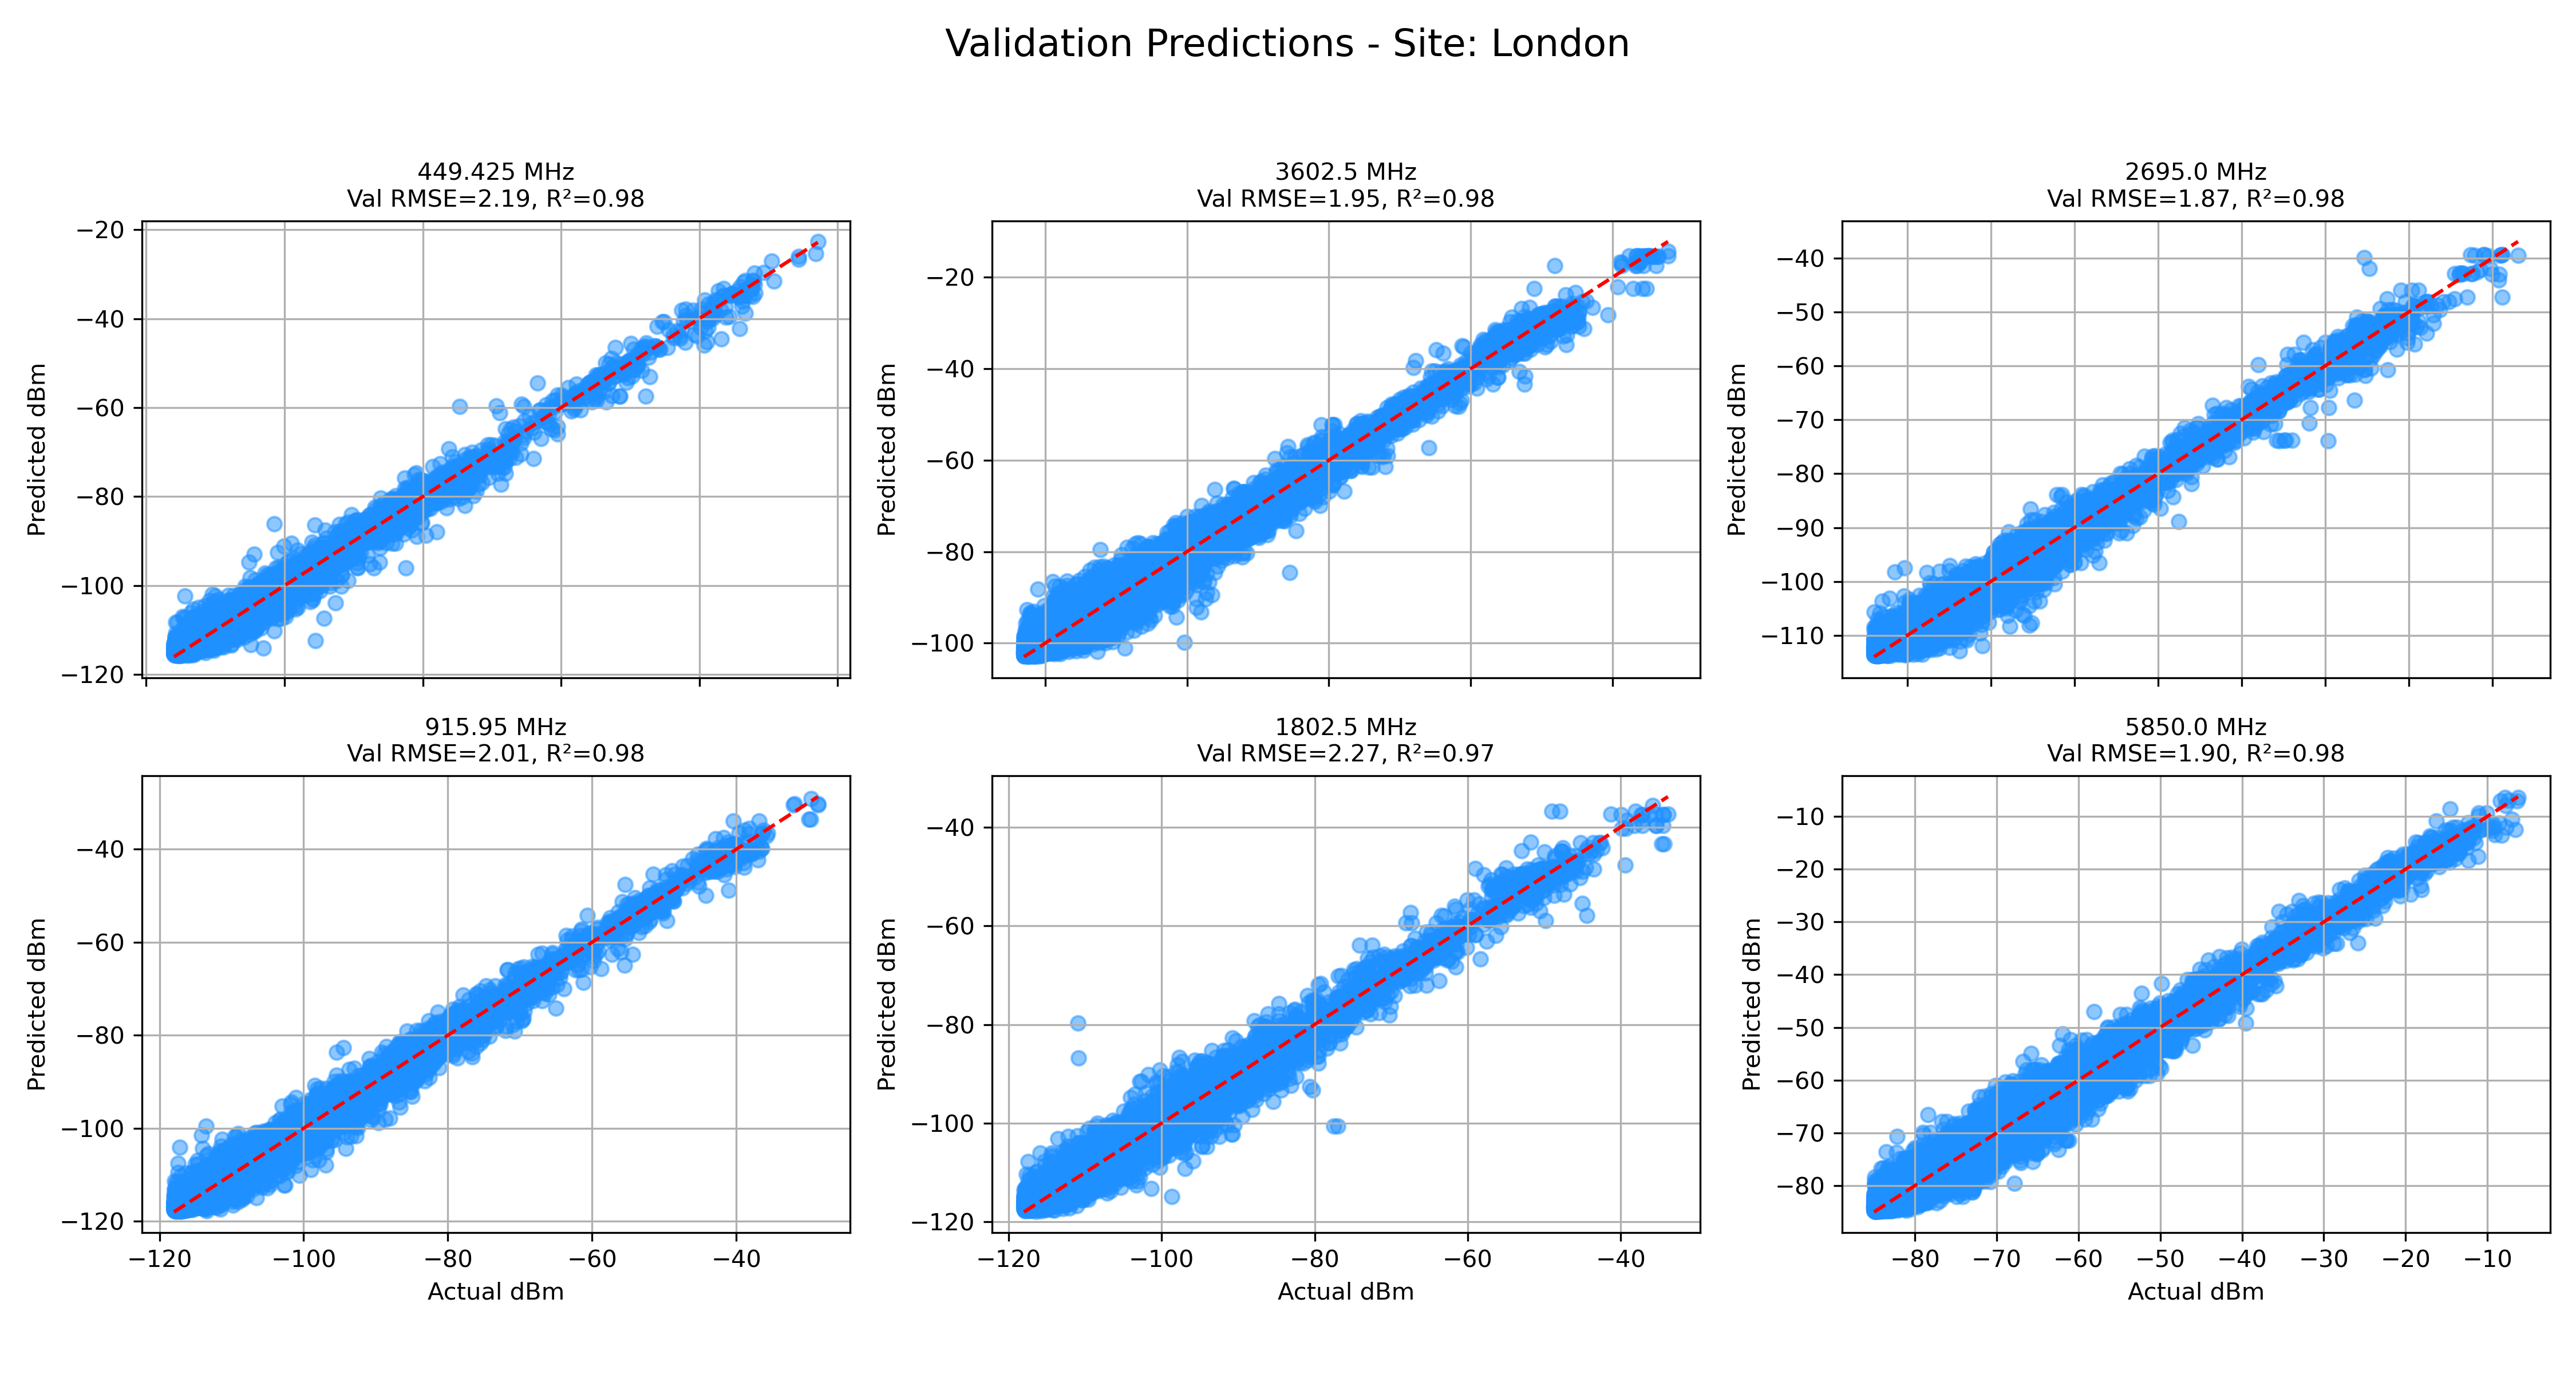
\includegraphics[width=.9\linewidth, height = 0.25\textheight]{Figures/Methodology/RF_F_S_Level/London_val.png}}
    \caption{Validation Results London}
    \label{fig:data-read}
\end{figure}

\begin{figure}[H]
    \centering
    \fbox{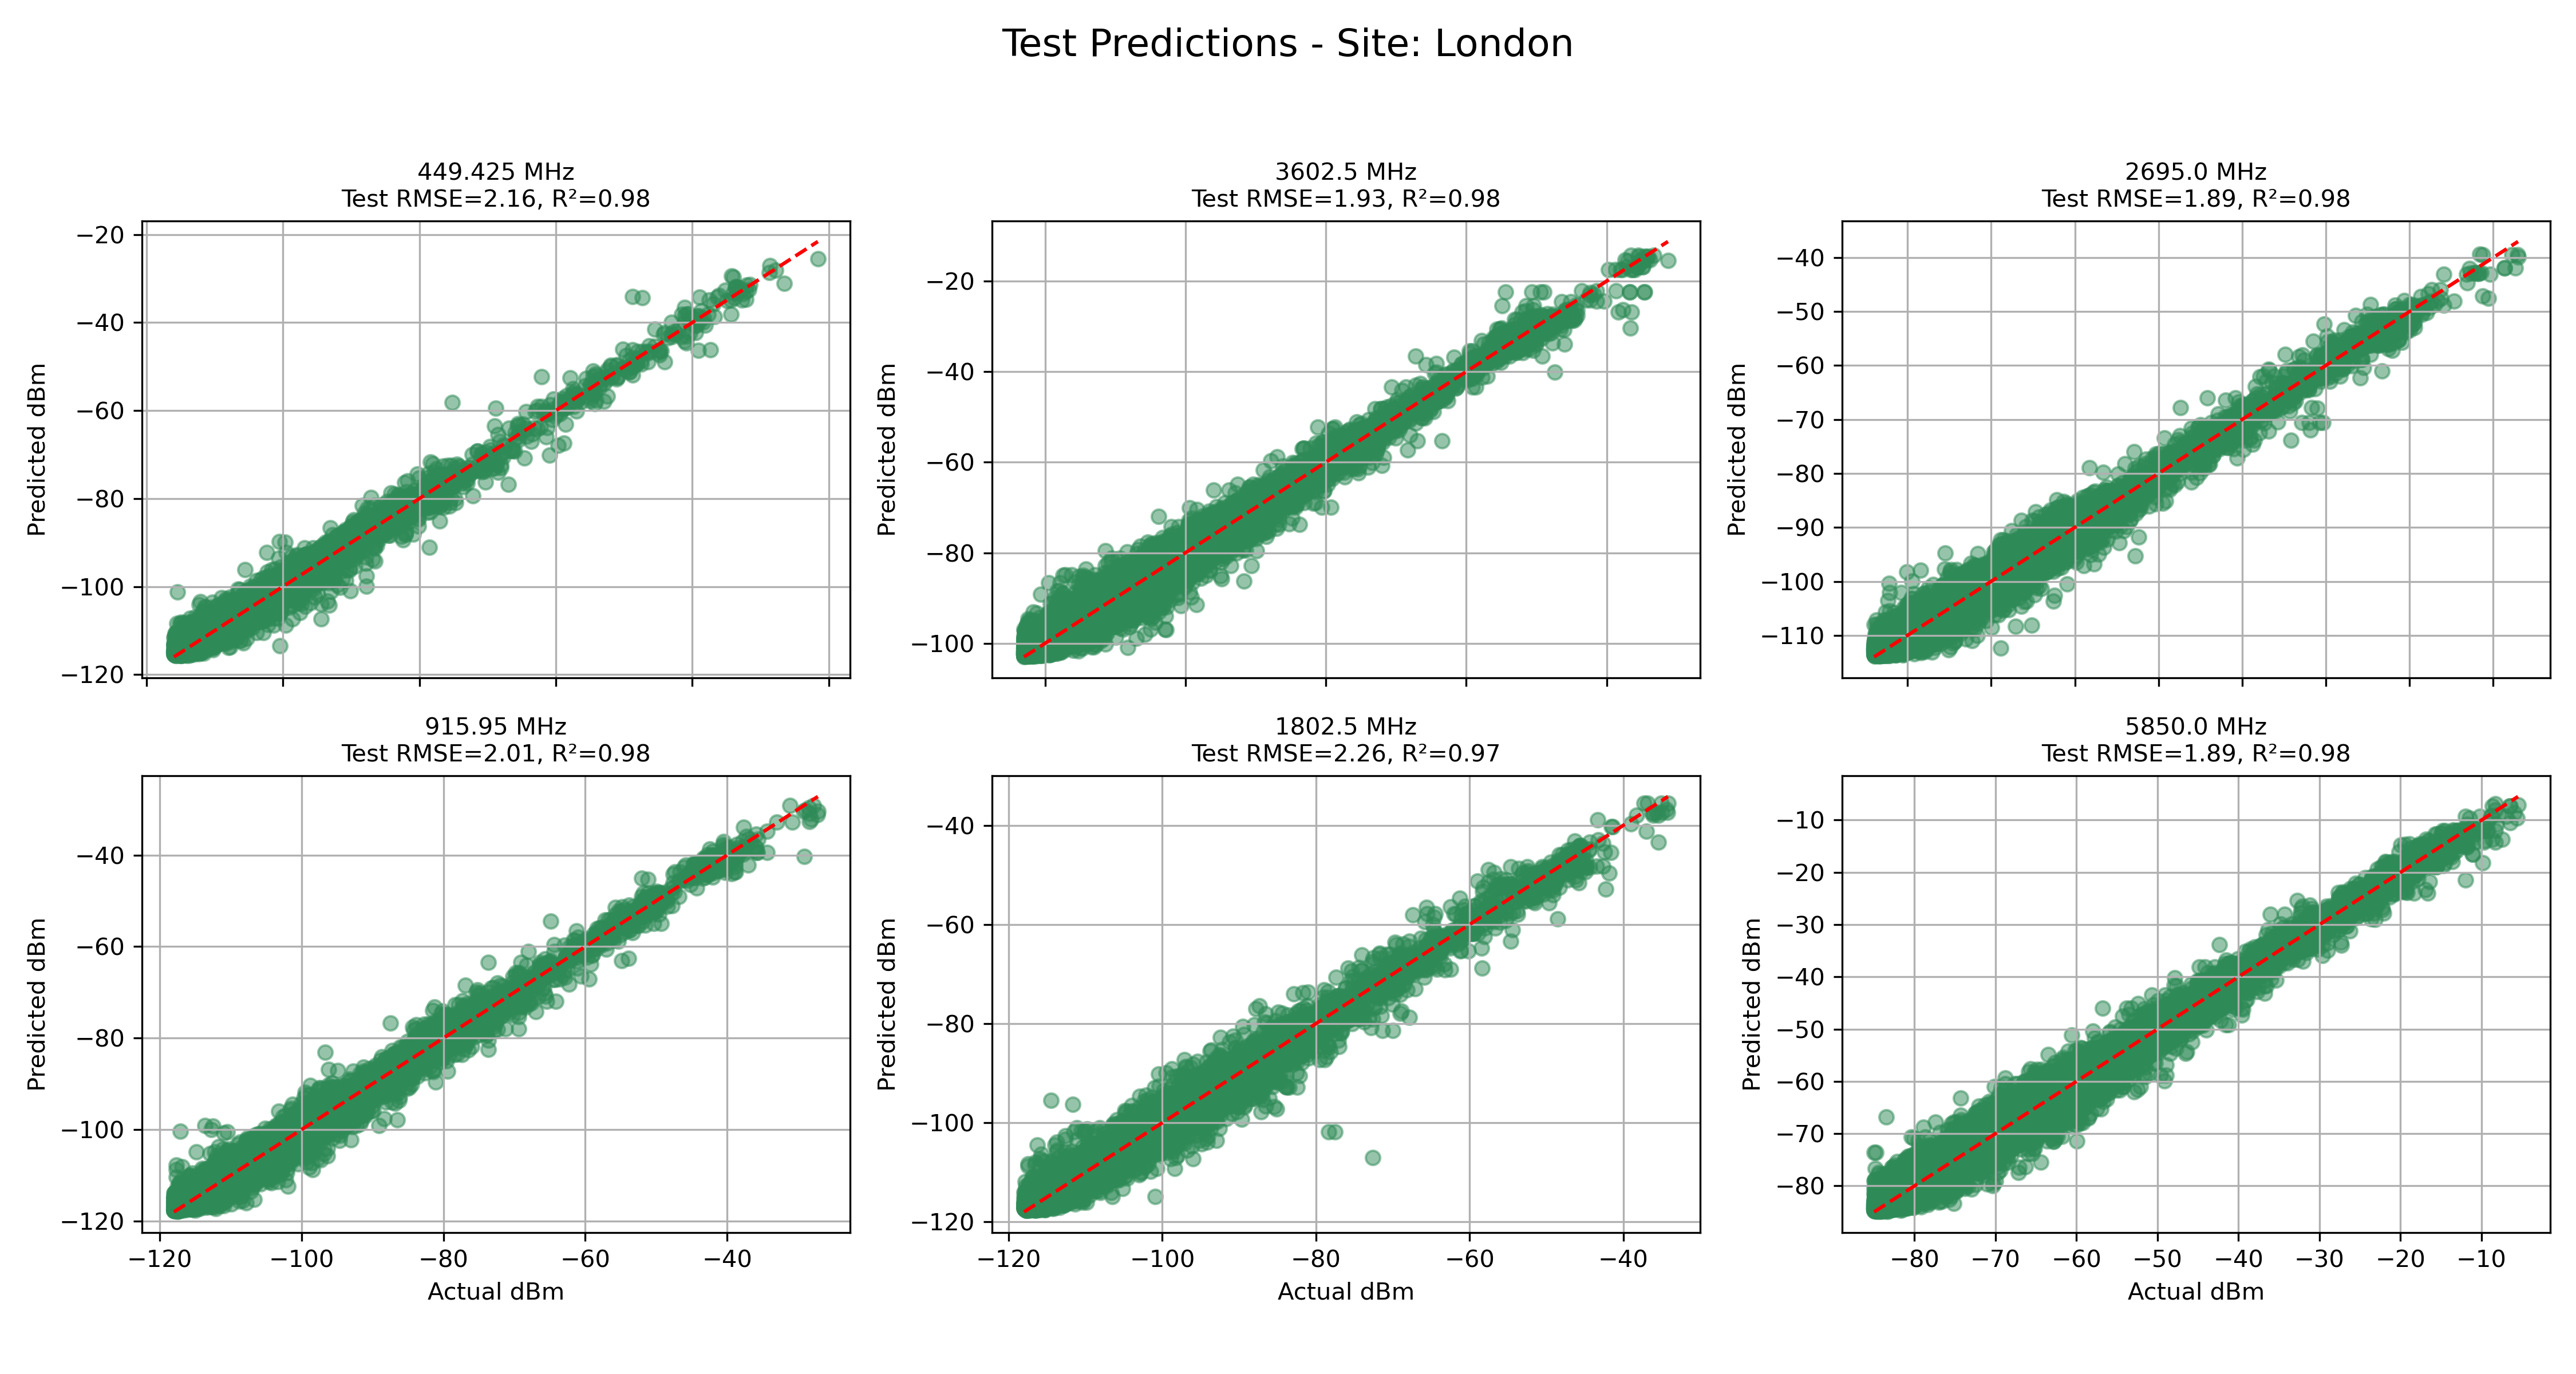
\includegraphics[width=.9\linewidth, height = 0.25\textheight]{Figures/Methodology/RF_F_S_Level/London_test.png}}
    \caption{Test Results London}
    \label{fig:data-read}
\end{figure}

\begin{table}[h]
    \centering
    \begin{tabular}{|c|c|c|c|c|c|}
        \hline
        \rowcolor{myblue}
        \textcolor{white}{\textbf{Frequency (MHz)}} & 
        \textcolor{white}{\textbf{Val RMSE}} & 
        \textcolor{white}{\textbf{Val R²}} & 
        \textcolor{white}{\textbf{Test RMSE}} & 
        \textcolor{white}{\textbf{Test R²}} & 
        \textcolor{white}{\textbf{Num Samples}} \\ \hline
        449.425        & 2.19 & 0.98 & 2.16 & 0.98 & 26,149   \\ \cdashline{1-6}[.4pt/2pt]
        915.950        & 2.01 & 0.98 & 2.01 & 0.98 & 54,402   \\ \cdashline{1-6}[.4pt/2pt]
        1802.500       & 2.27 & 0.97 & 2.26 & 0.97 & 56,945   \\ \cdashline{1-6}[.4pt/2pt]
        2695.000       & 1.87 & 0.98 & 1.89 & 0.98 & 61,588   \\ \cdashline{1-6}[.4pt/2pt]
        3602.500       & 1.95 & 0.98 & 1.93 & 0.98 & 128,340  \\ \cdashline{1-6}[.4pt/2pt]
        5850.000       & 1.90 & 0.98 & 1.89 & 0.98 & 130,849  \\ \hline
    \end{tabular}
    \caption{Model Performance Results London}
    \label{tab:frequency_stats}
\end{table}

\begin{itemize}
    \item \textbf{Observation:} \texttt{Figure 5.10}, \texttt{Figure 5.11} and \texttt{Table 5.3} are the model result for site London.
    \begin{itemize}
        \item  When compared the test and validation sets the performance seems very similar on both the sets,with $R^2 \simeq 0.97$ - $0.98$. Showing low error with RMSE $\simeq 1.8$ - $2.3$ indicating very low deviation in actual vs predicted value of signal strength.
        \item Performance across different frequency remain consistently good with very minimal error even at higher bands even with high propagation complexity.
    \end{itemize}
\end{itemize}

\begin{figure}[H]
    \centering
    \fbox{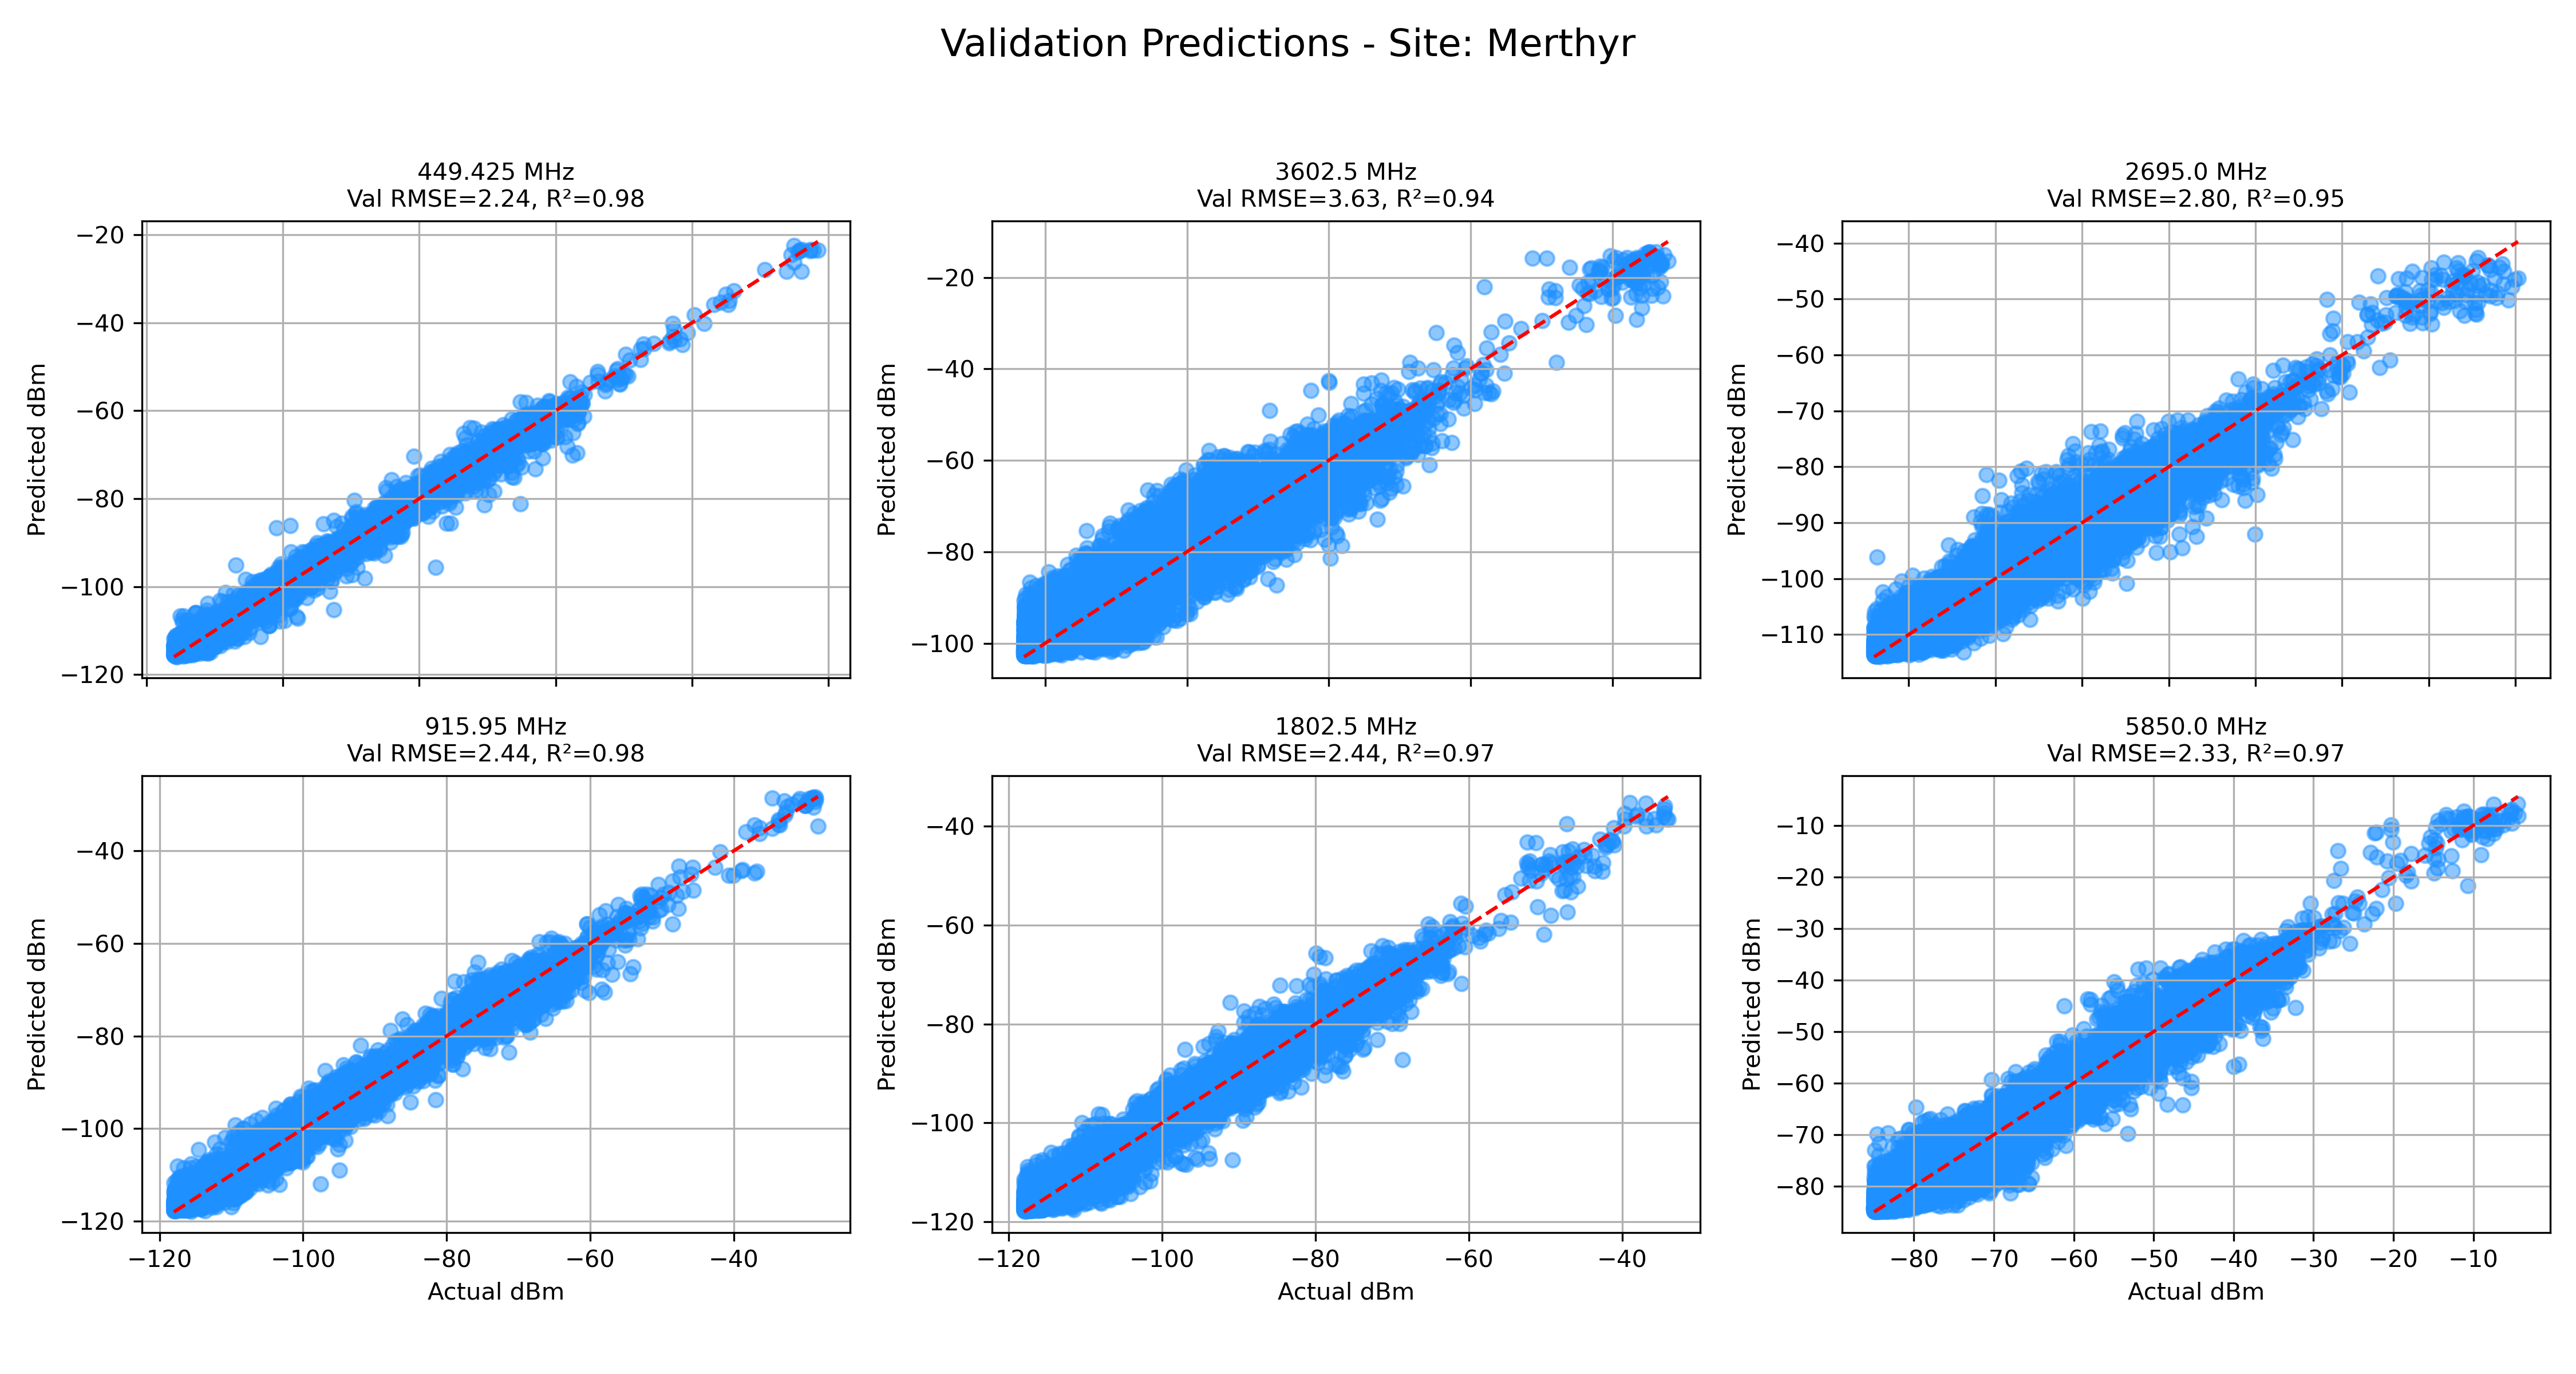
\includegraphics[width=.9\linewidth, height = 0.25\textheight]{Figures/Methodology/RF_F_S_Level/Merthyr_val.png}}
    \caption{Validation Results Merthyr}
    \label{fig:data-read}
\end{figure}

\begin{figure}[H]
    \centering
    \fbox{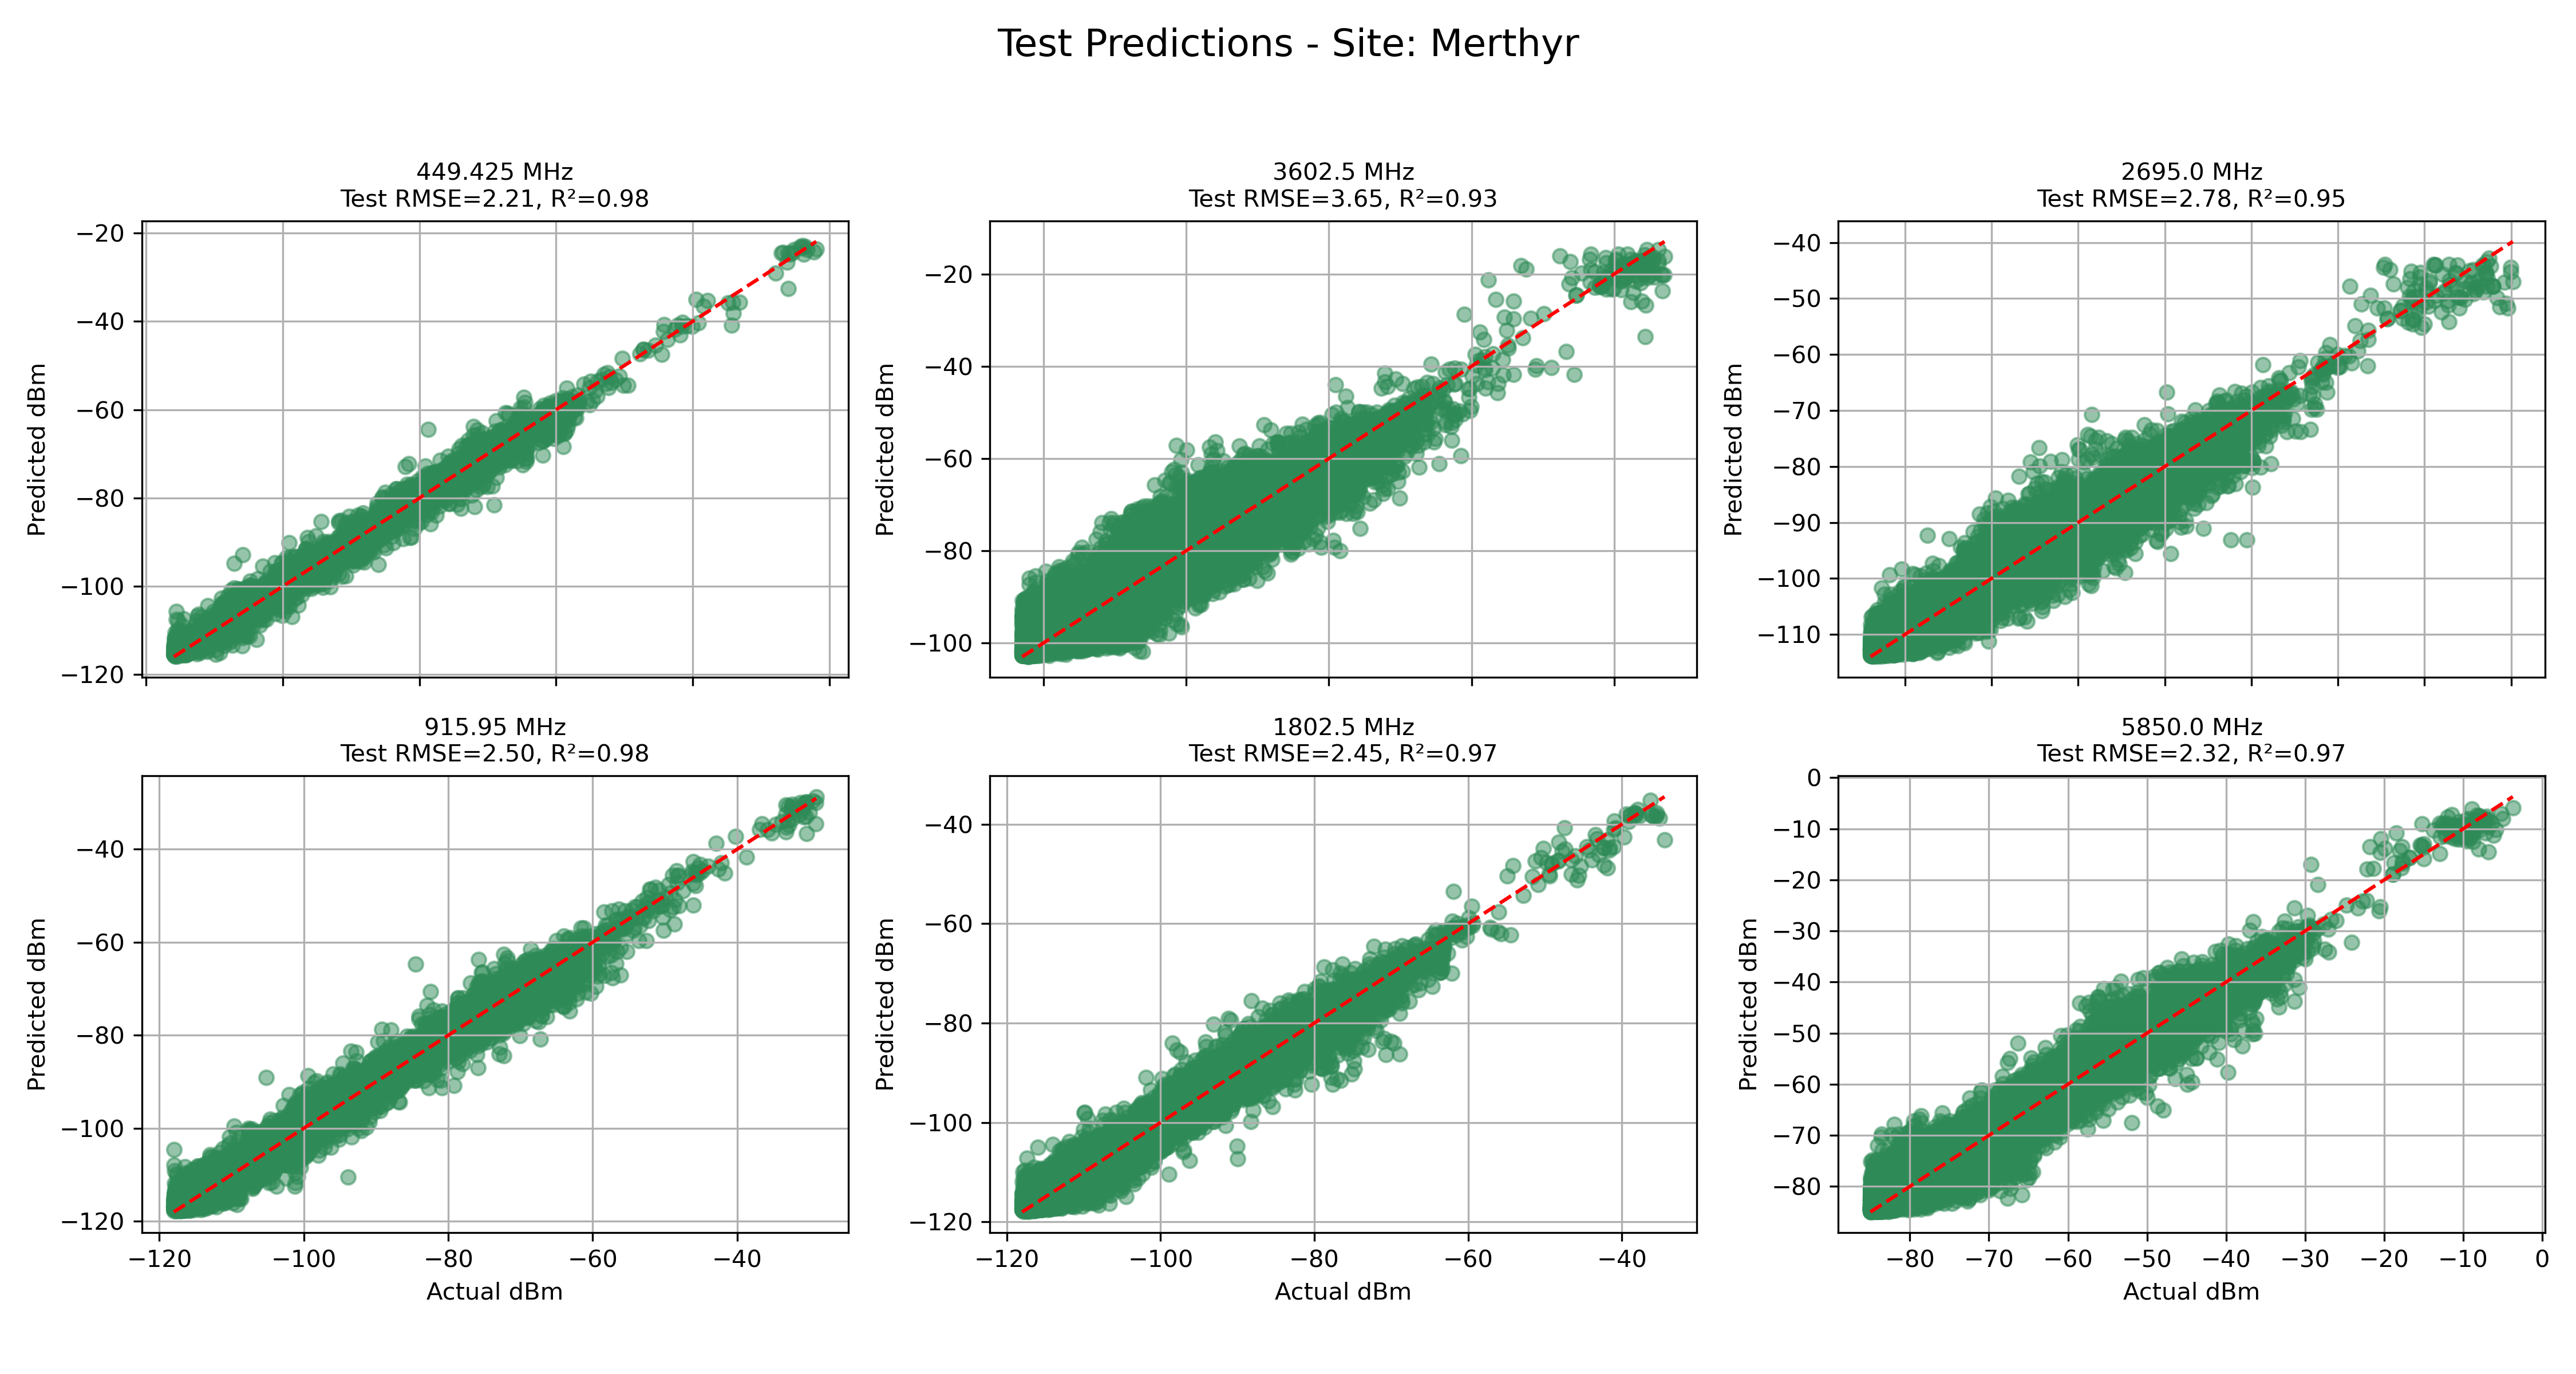
\includegraphics[width=.9\linewidth, height = 0.25\textheight]{Figures/Methodology/RF_F_S_Level/Merthyr_test.png}}
    \caption{Test Results Merthyr}
    \label{fig:data-read}
\end{figure}

\begin{table}[h]
    \centering
    \begin{tabular}{|c|c|c|c|c|c|}
        \hline
        \rowcolor{myblue}
        \textcolor{white}{\textbf{Frequency (MHz)}} & 
        \textcolor{white}{\textbf{Val RMSE}} & 
        \textcolor{white}{\textbf{Val R²}} & 
        \textcolor{white}{\textbf{Test RMSE}} & 
        \textcolor{white}{\textbf{Test R²}} & 
        \textcolor{white}{\textbf{Num Samples}} \\ \hline
        449.425        & 2.24 & 0.98 & 2.21 & 0.98 & 21,392   \\ \cdashline{1-6}[.4pt/2pt]
        915.950        & 2.44 & 0.98 & 2.50 & 0.98 & 42,725   \\ \cdashline{1-6}[.4pt/2pt]
        1802.500       & 2.44 & 0.97 & 2.45 & 0.97 & 72,571   \\ \cdashline{1-6}[.4pt/2pt]
        2695.000       & 2.80 & 0.95 & 2.78 & 0.95 & 83,589   \\ \cdashline{1-6}[.4pt/2pt]
        3602.500       & 3.63 & 0.94 & 3.65 & 0.93 & 121,184  \\ \cdashline{1-6}[.4pt/2pt]
        5850.000       & 2.33 & 0.97 & 2.32 & 0.97 & 178,484  \\ \hline
    \end{tabular}
    \caption{Model Performance Results Merthyr}
    \label{tab:frequency_stats}
\end{table}

\begin{itemize}
    \item \textbf{Observation:} \texttt{Figure 5.12}, \texttt{Figure 5.13} and \texttt{Table 5.4} are the model result for site Merthyr.
    \begin{itemize} 
        \item  Across all the frequency bands, plots shows high consistency for both test and validation sets, indicating high accuracy and low error in prediction. RMSE values ranging between 2.24 to 3.36 with lowest at 449.425MHz and highest at 3602.5MHz. Also, high $R^2$ value suggest model explains the variability in data accurately. 
        \item Overall, Merthyr sites shows consistently good prediction results with slight deviation at higher frequency bands due to complex propagation.
    \end{itemize}
\end{itemize}

\begin{figure}[H]
    \centering
    \fbox{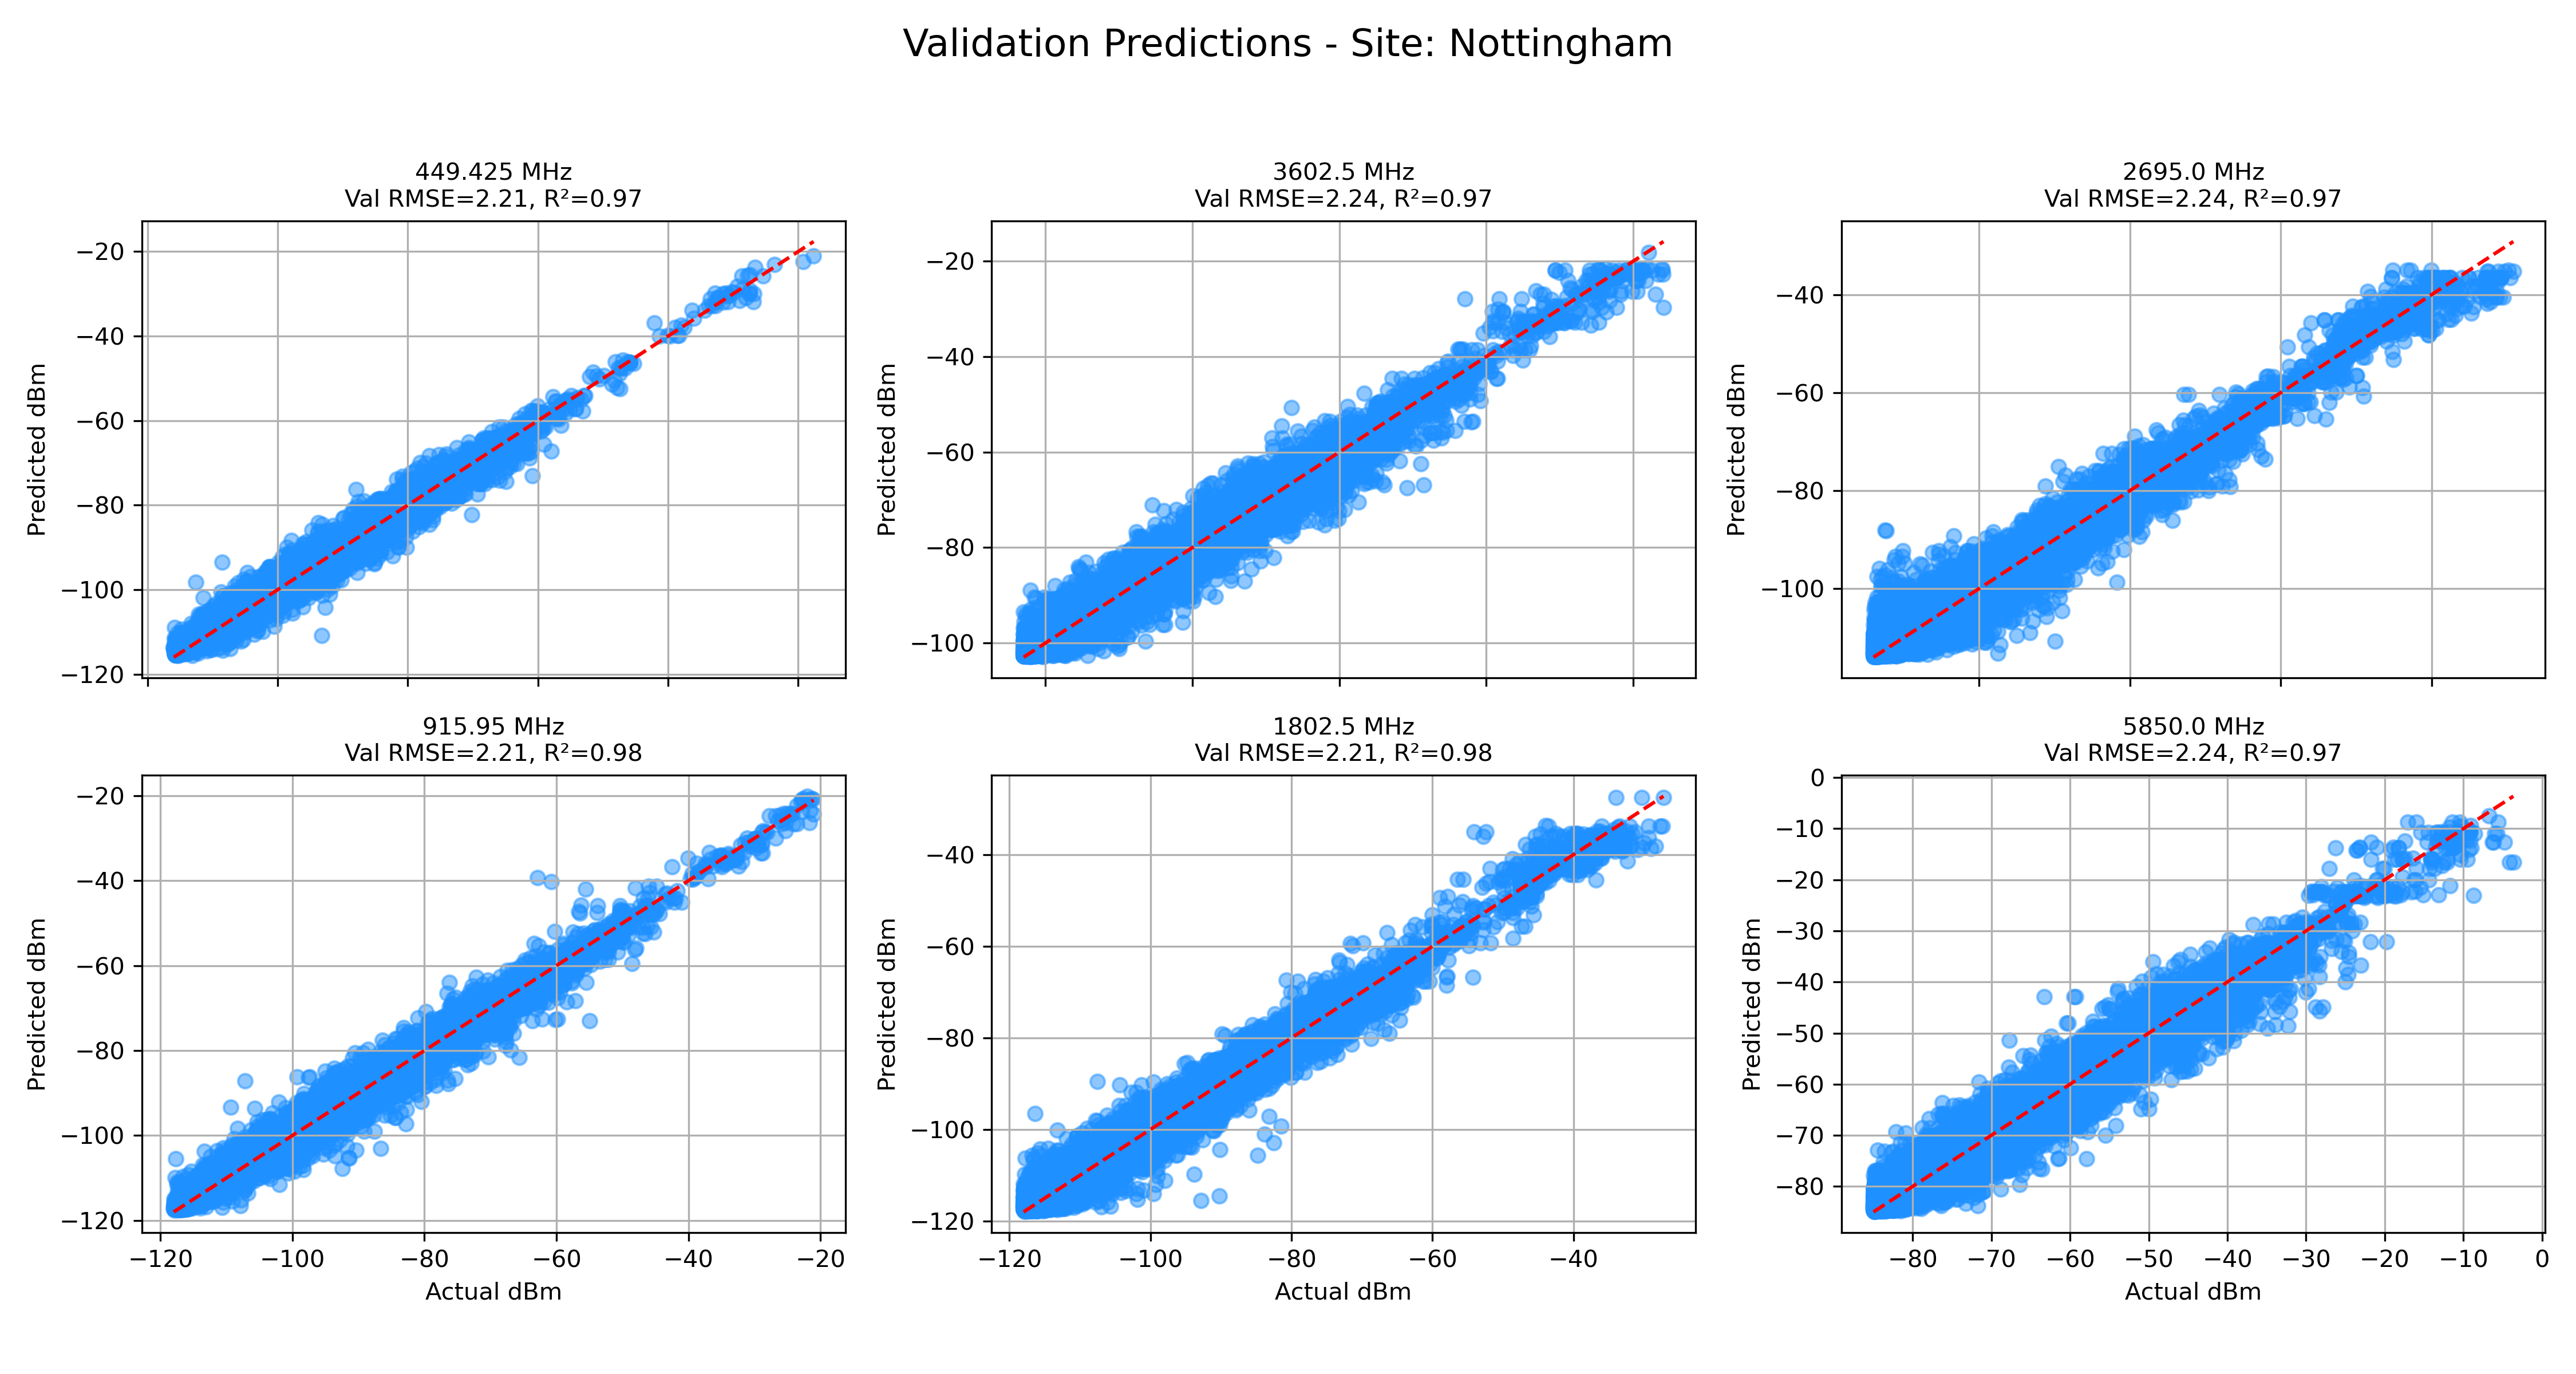
\includegraphics[width=.9\linewidth, height = 0.25\textheight]{Figures/Methodology/RF_F_S_Level/Nottingham_val.png}}
    \caption{Validation Results Nottingham}
    \label{fig:data-read}
\end{figure}

\begin{figure}[H]
    \centering
    \fbox{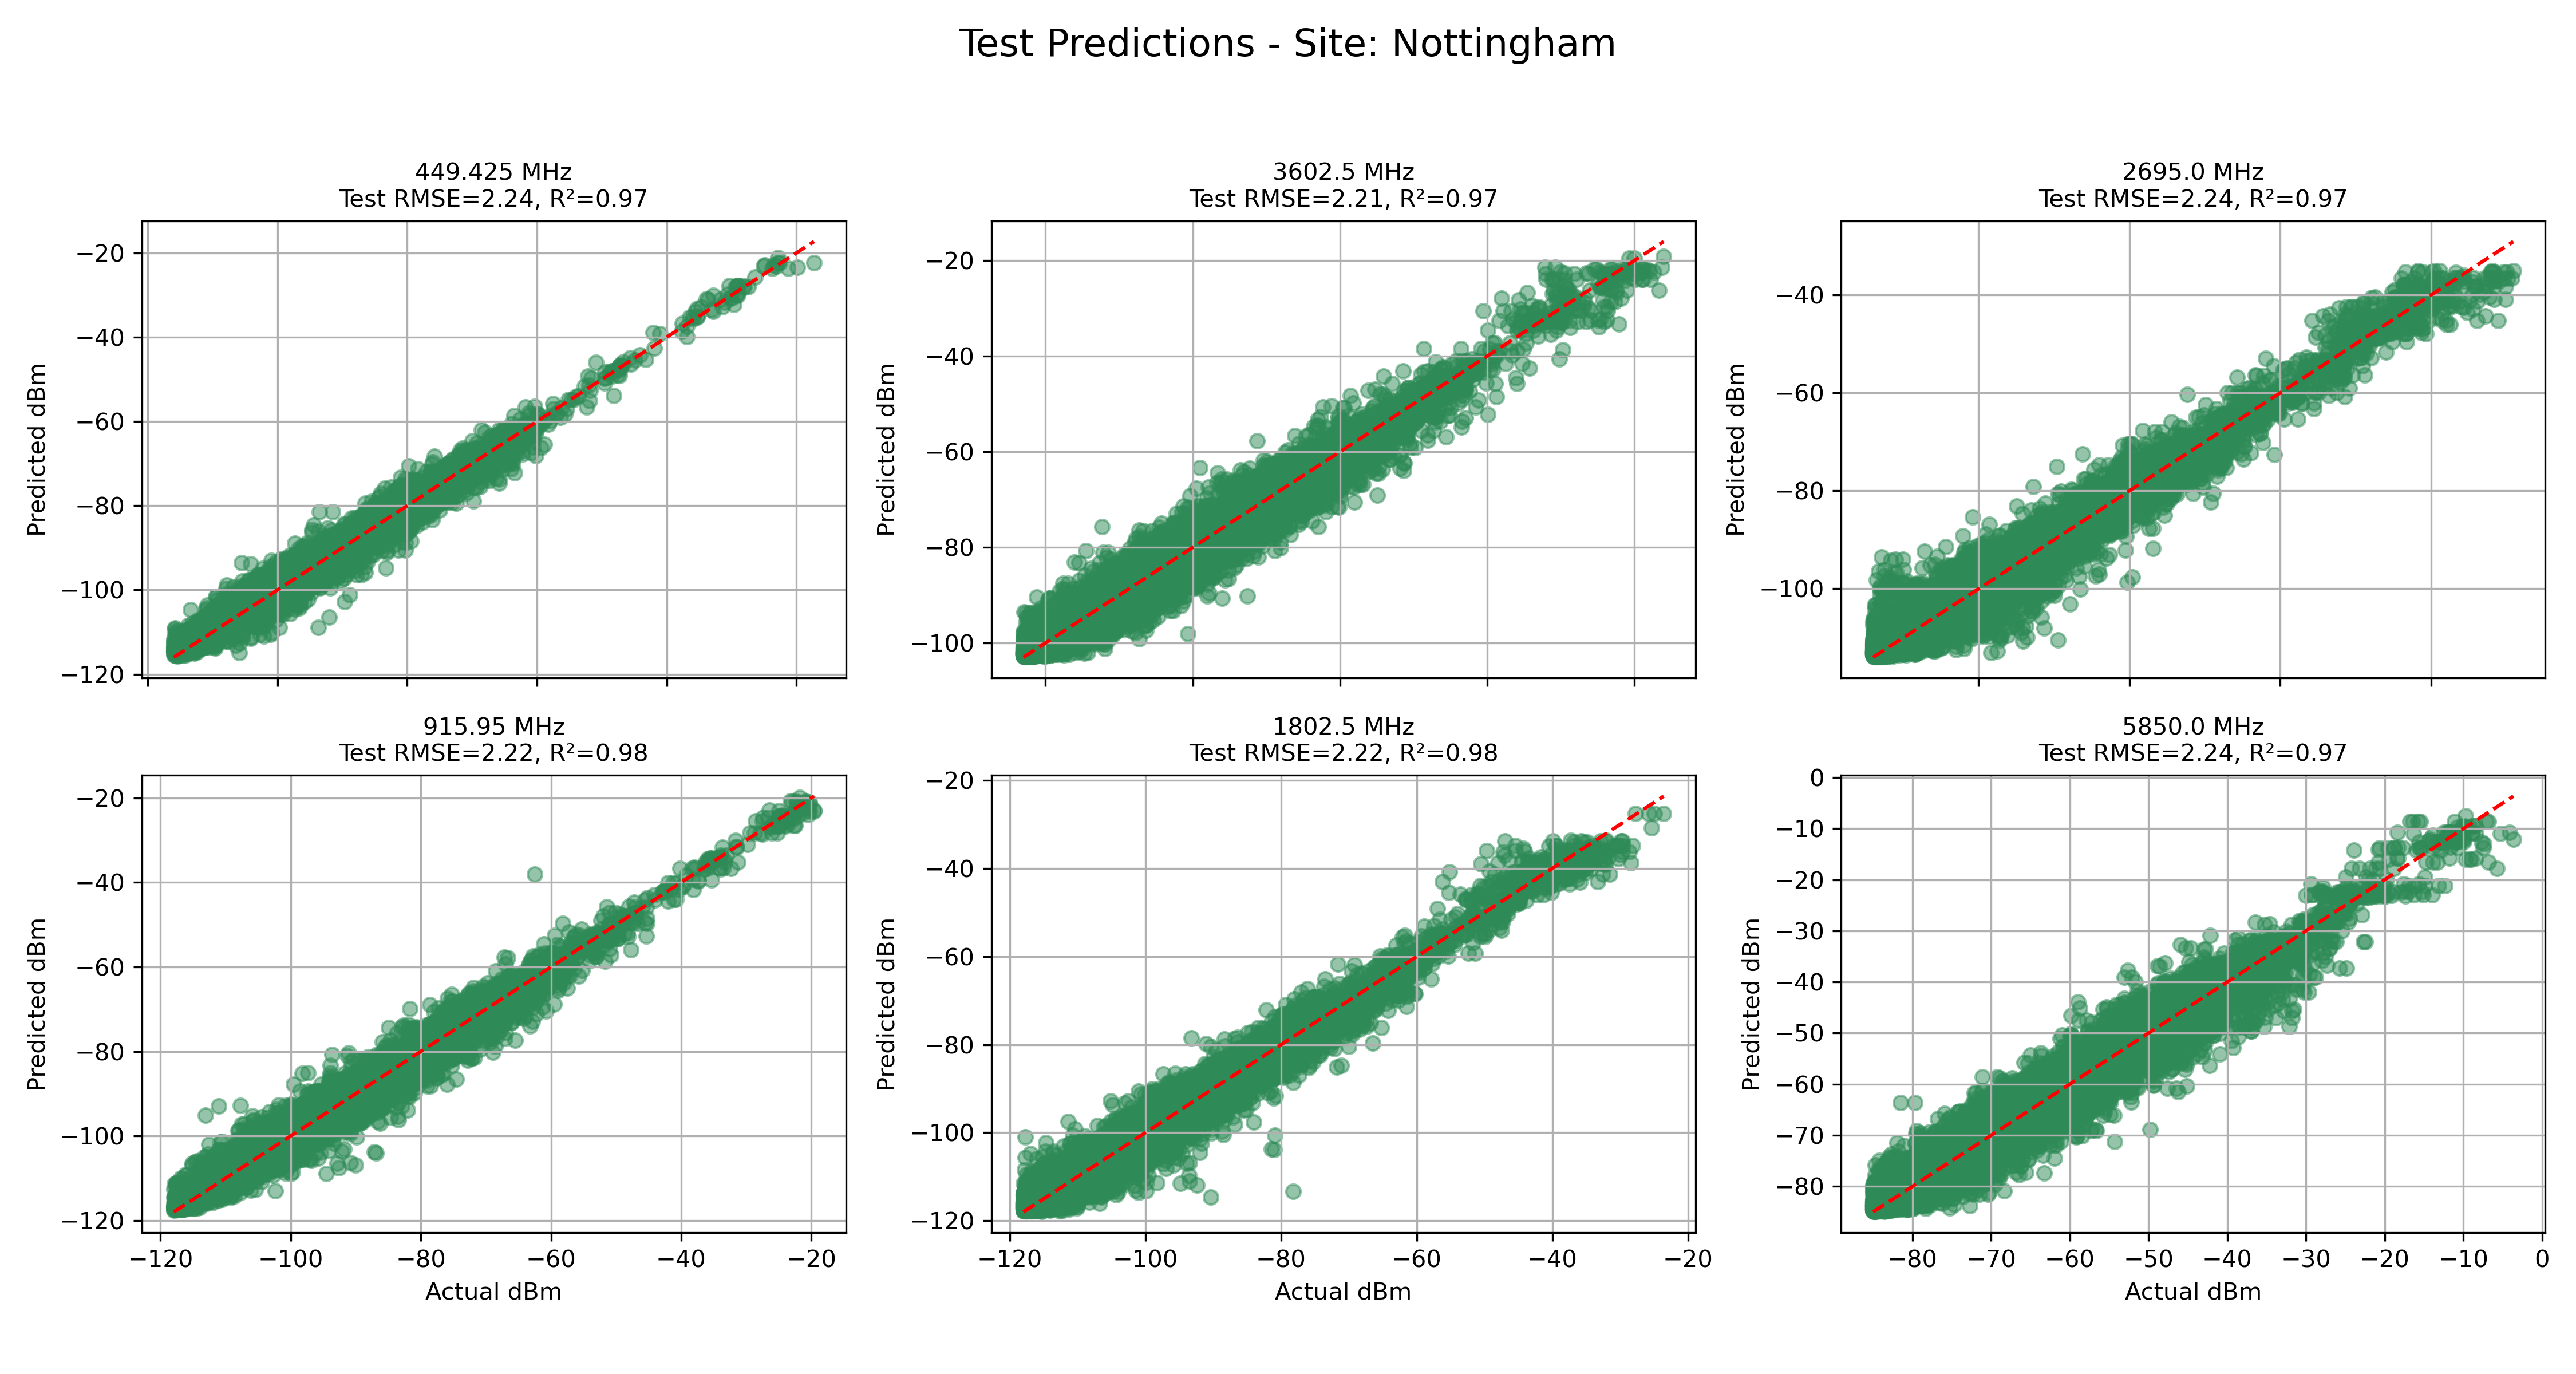
\includegraphics[width=.9\linewidth, height = 0.25\textheight]{Figures/Methodology/RF_F_S_Level/Nottingham_test.png}}
    \caption{Test Results Nottingham}
    \label{fig:data-read}
\end{figure}

\begin{table}[h]
    \centering
    \begin{tabular}{|c|c|c|c|c|c|}
        \hline
        \rowcolor{myblue}
        \textcolor{white}{\textbf{Frequency (MHz)}} & 
        \textcolor{white}{\textbf{Val RMSE}} & 
        \textcolor{white}{\textbf{Val R²}} & 
        \textcolor{white}{\textbf{Test RMSE}} & 
        \textcolor{white}{\textbf{Test R²}} & 
        \textcolor{white}{\textbf{Num Samples}} \\ \hline
        449.425        & 2.21 & 0.97 & 2.24 & 0.97 & 45,297   \\ \cdashline{1-6}[.4pt/2pt]
        915.950        & 2.21 & 0.98 & 2.22 & 0.98 & 92,970   \\ \cdashline{1-6}[.4pt/2pt]
        1802.500       & 2.21 & 0.98 & 2.22 & 0.98 & 144,312  \\ \cdashline{1-6}[.4pt/2pt]
        2695.000       & 2.24 & 0.97 & 2.24 & 0.97 & 165,968  \\ \cdashline{1-6}[.4pt/2pt]
        3602.500       & 2.24 & 0.97 & 2.21 & 0.97 & 162,004  \\ \cdashline{1-6}[.4pt/2pt]
        5850.000       & 2.24 & 0.97 & 2.24 & 0.97 & 217,394  \\ \hline
    \end{tabular}
    \caption{Model Performance Results Nottingham}
    \label{tab:frequency_stats}
\end{table}

\begin{itemize}
    \item \textbf{Observation:} \texttt{Figure 5.14}, \texttt{Figure 5.15} and \texttt{Table 5.5} are the model result for site Nottingham.
    \begin{itemize}
        \item  Both test and validation RMSE values are consistent across frequency bands, with slight difference from Merthyr. Additionally, high $R^2$ values suggest accurate model prediction and explanation of variability.  
        \item Unlike Merthyr, accuracy does not degrade at higher frequency bands but remain consistent in a small range (RMSE $\simeq 2.21$ - $2.24$)
    \end{itemize}
\end{itemize}

\begin{figure}[H]
    \centering
    \fbox{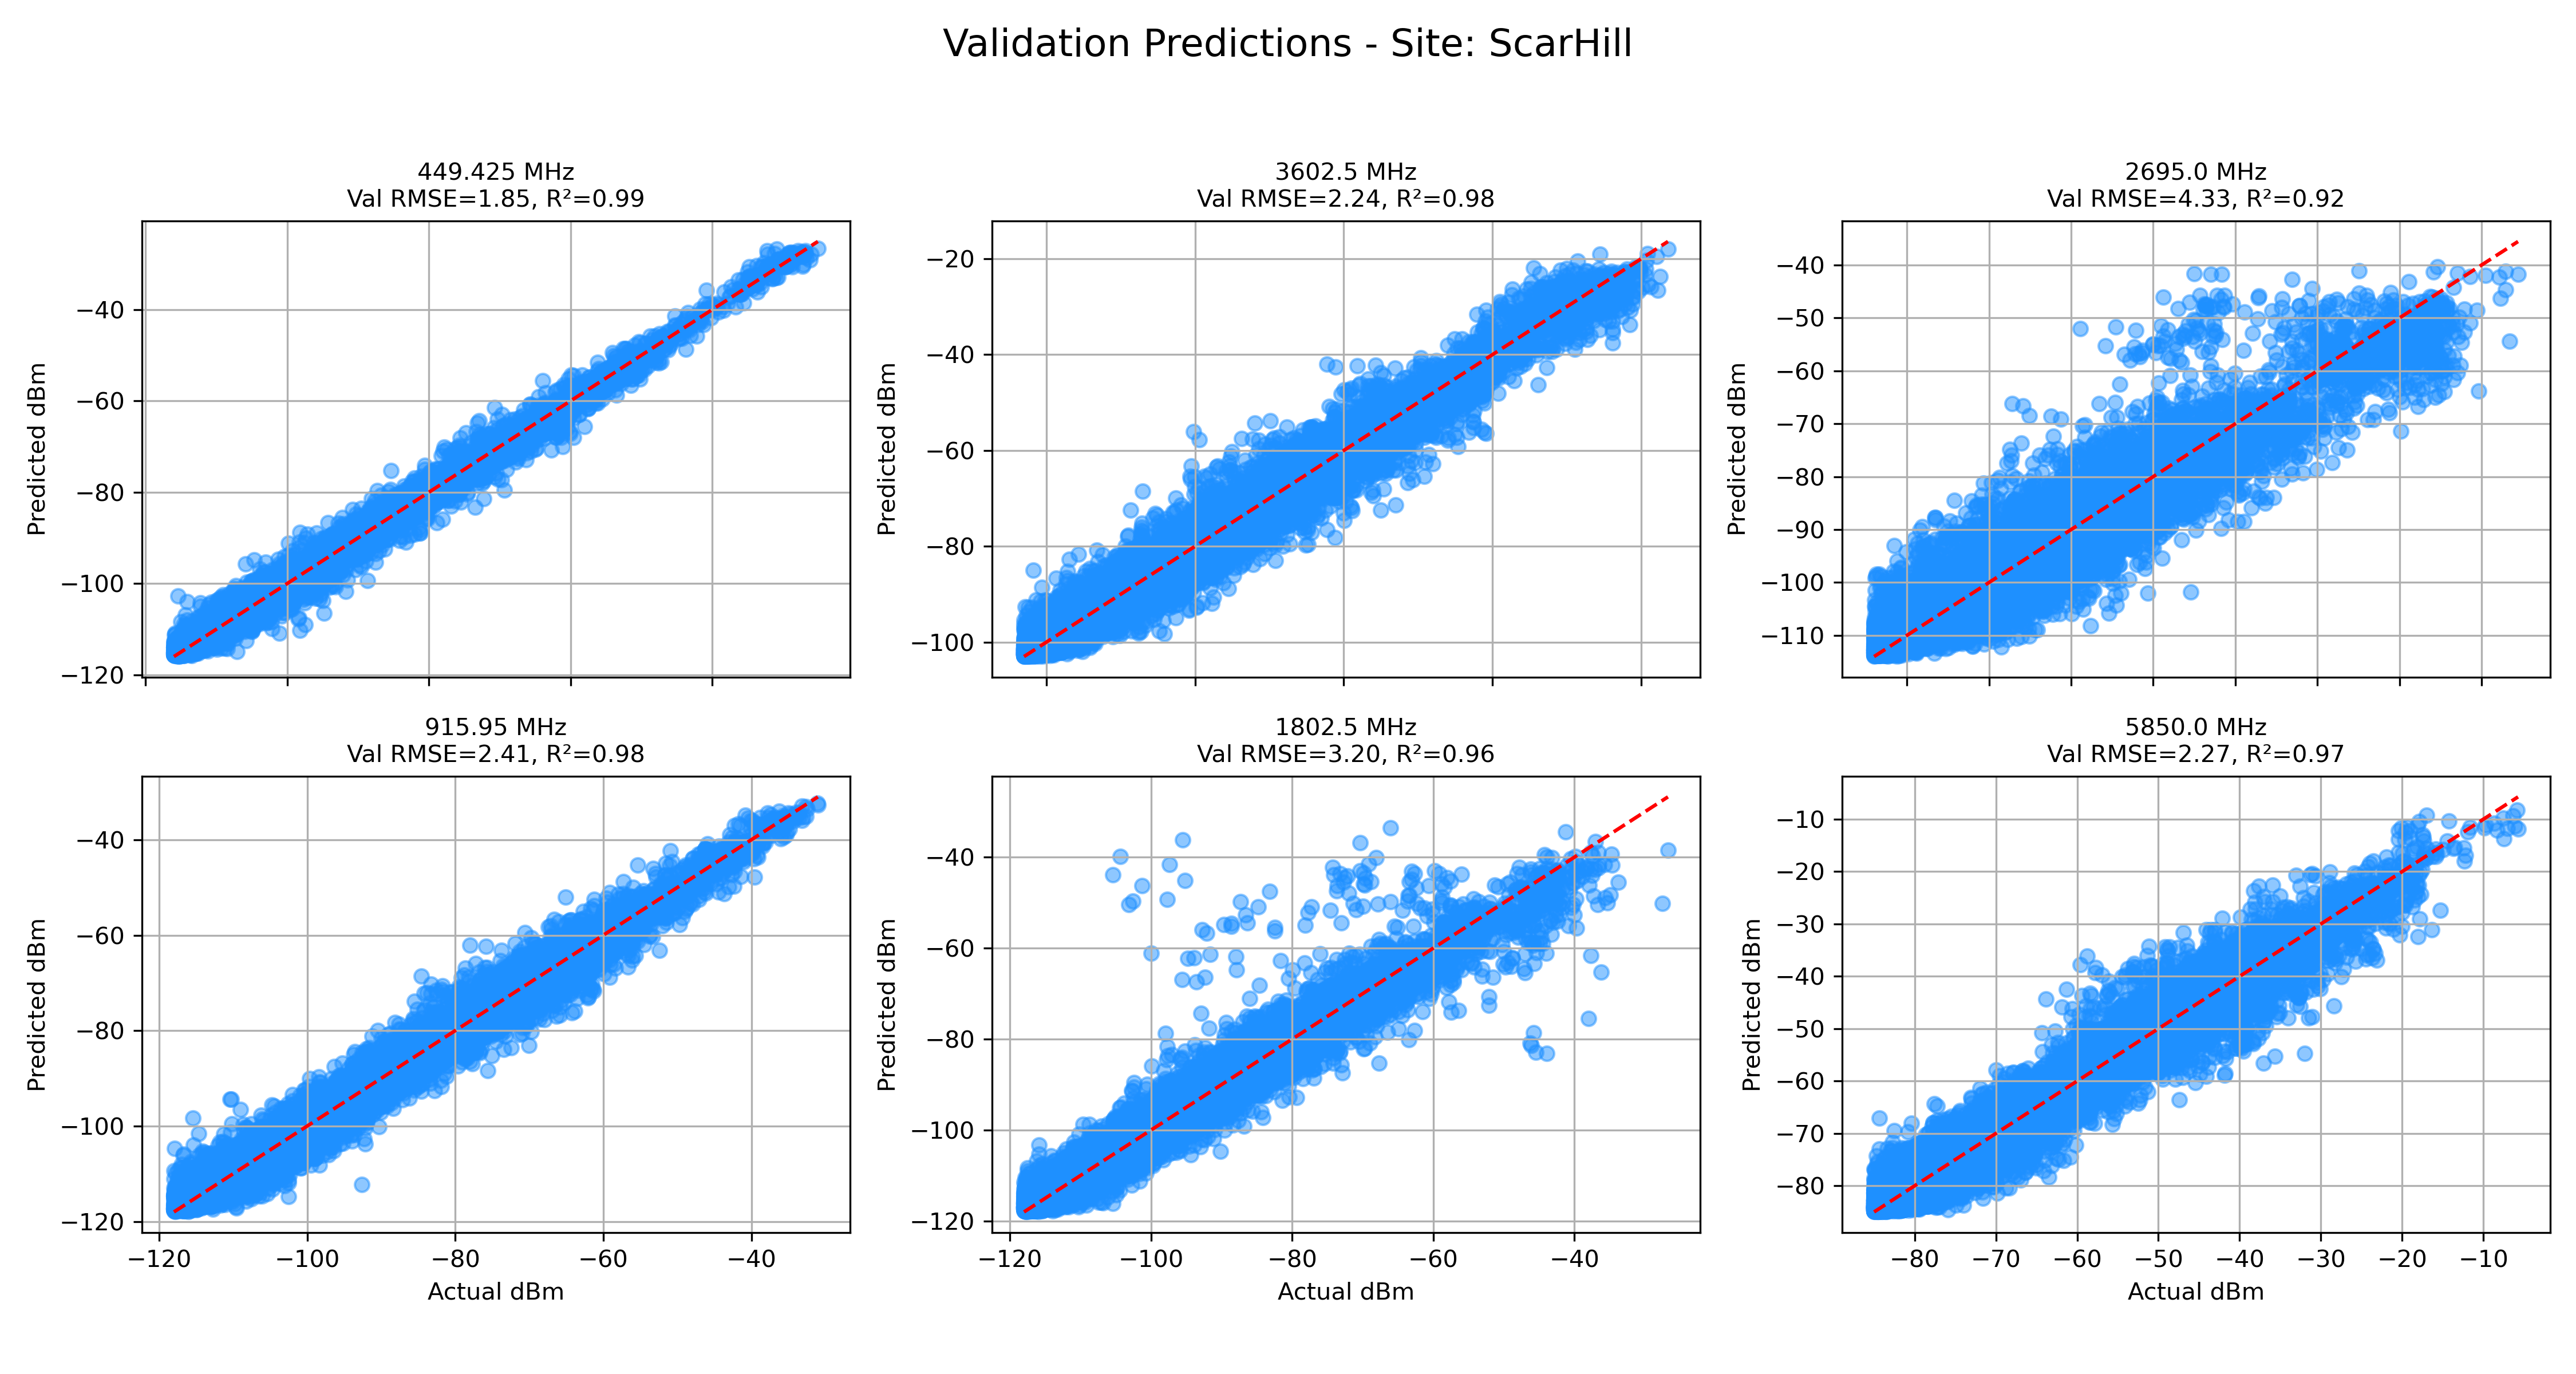
\includegraphics[width=.9\linewidth, height = 0.25\textheight]{Figures/Methodology/RF_F_S_Level/ScarHill_val.png}}
    \caption{Validation Results ScarHill}
    \label{fig:data-read}
\end{figure}

\begin{figure}[H]
    \centering
    \fbox{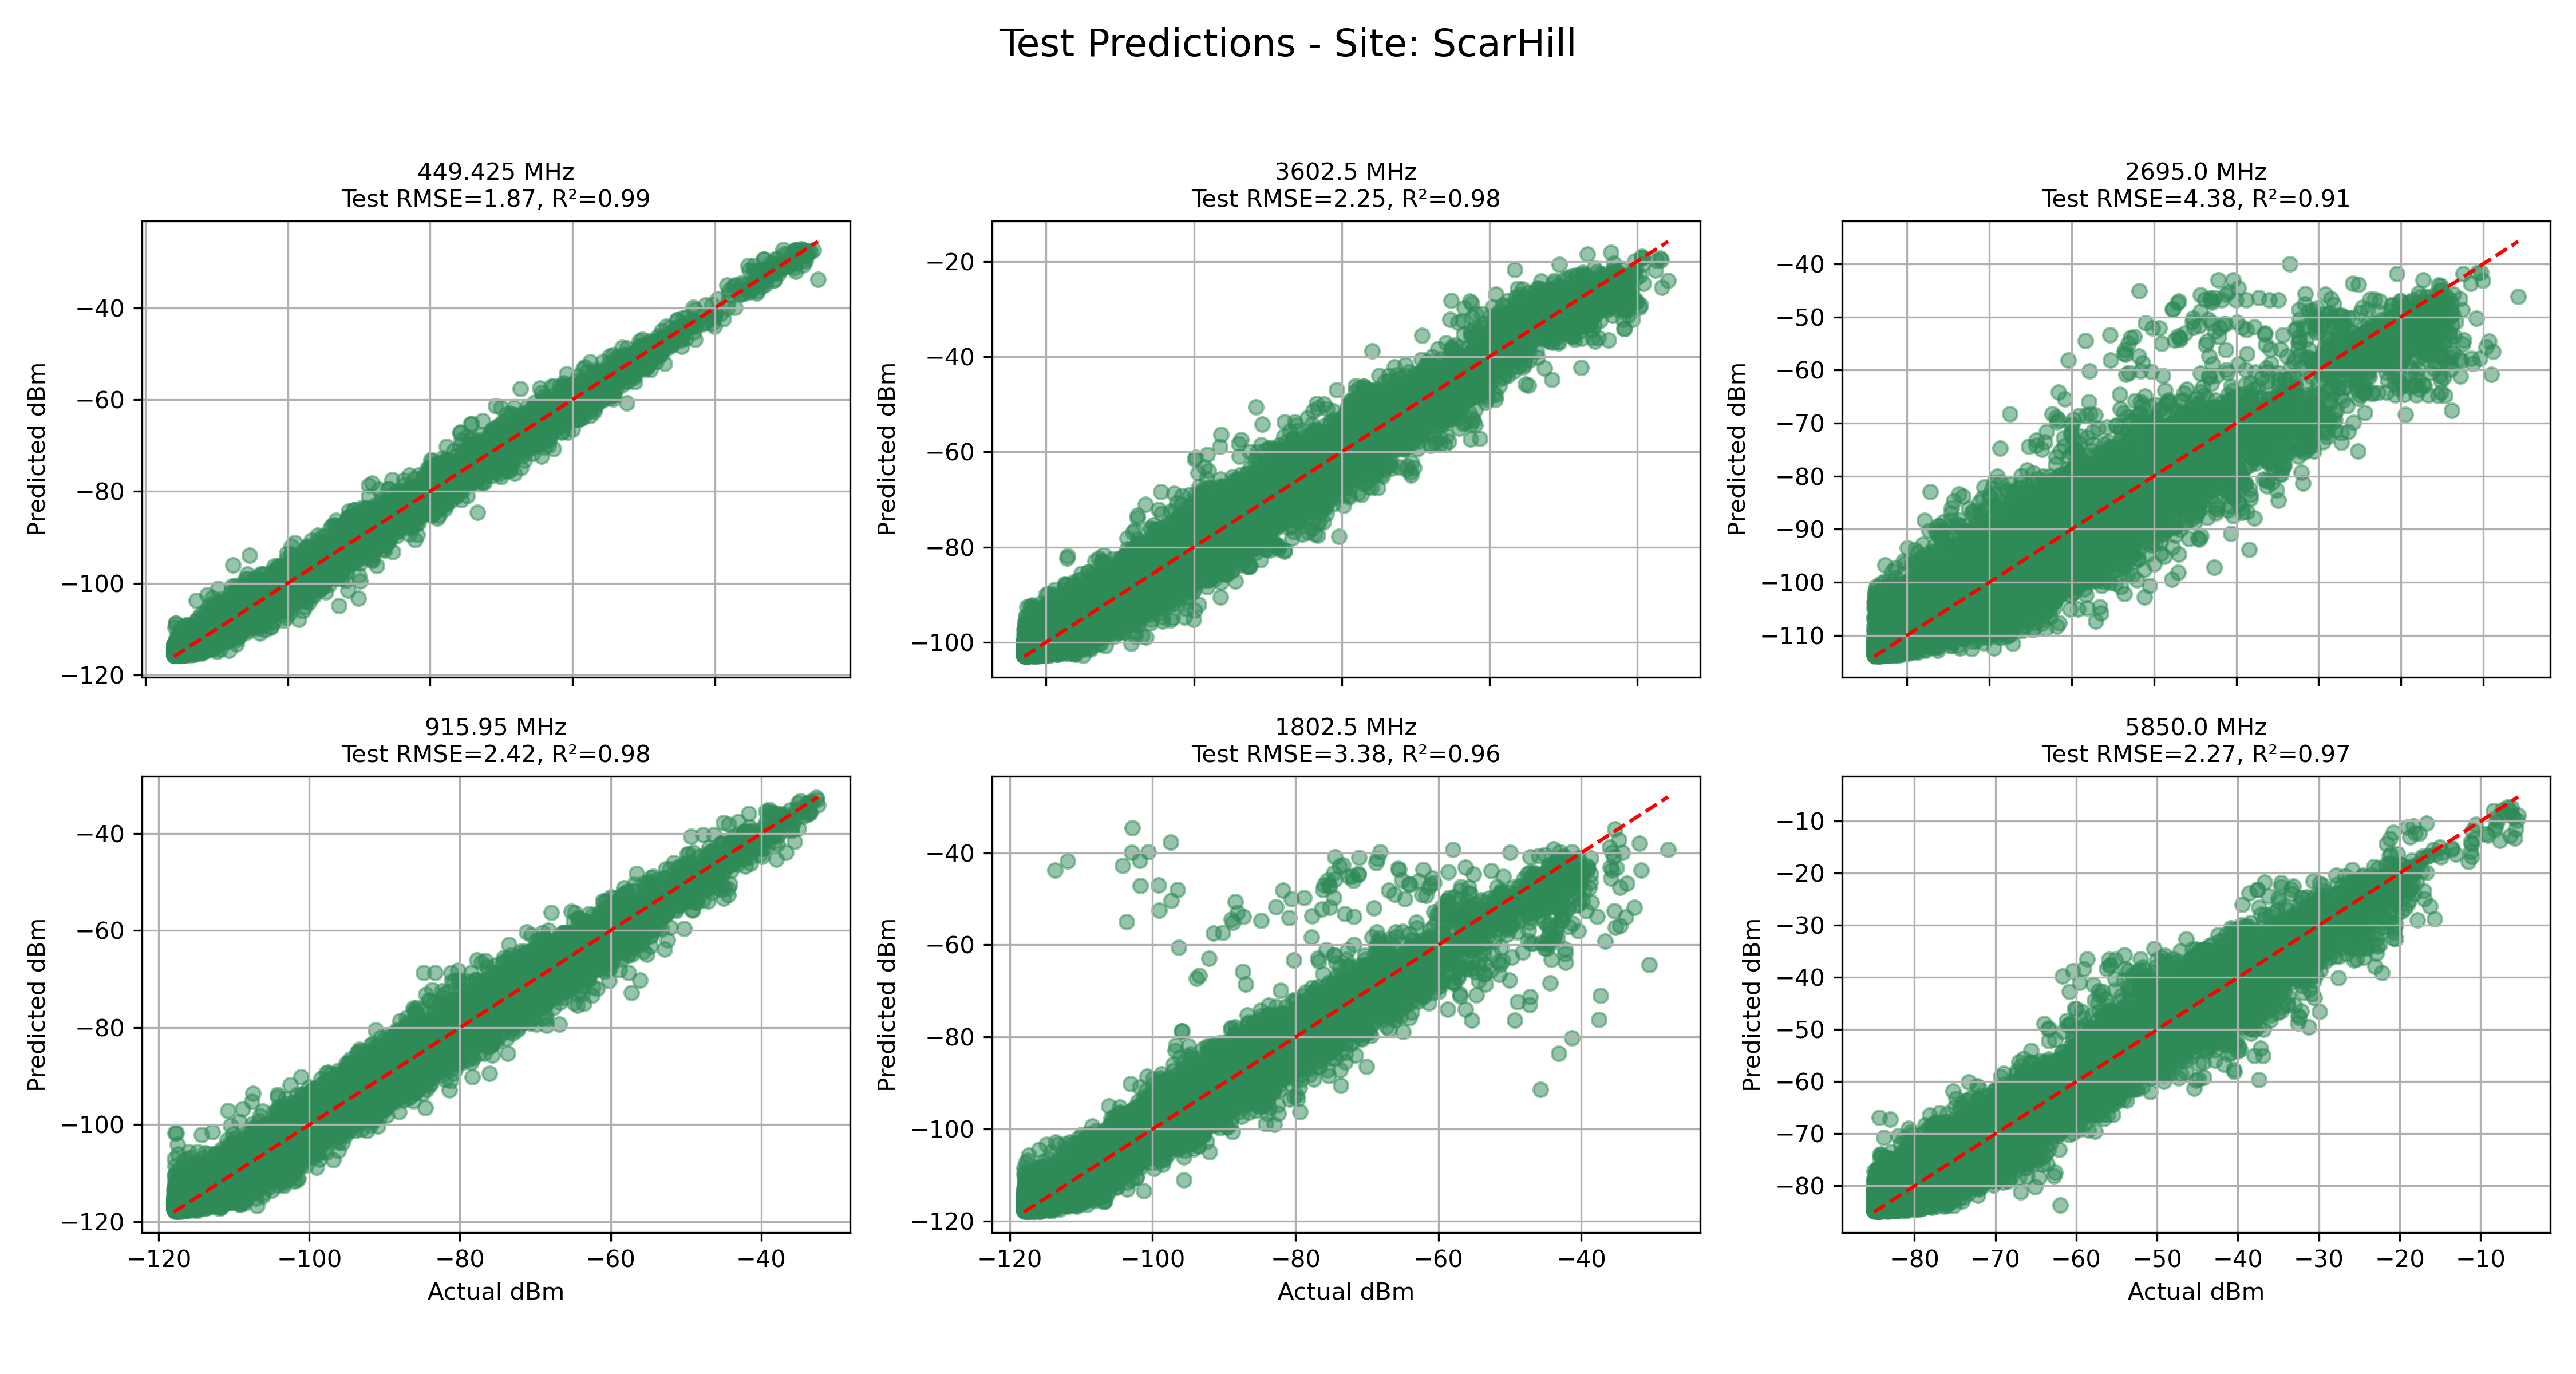
\includegraphics[width=.9\linewidth, height = 0.25\textheight]{Figures/Methodology/RF_F_S_Level/ScarHill_test.png}}
    \caption{Test Results ScarHill}
    \label{fig:data-read}
\end{figure}

\begin{table}[h]
    \centering
    \begin{tabular}{|c|c|c|c|c|c|}
        \hline
        \rowcolor{myblue}
        \textcolor{white}{\textbf{Frequency (MHz)}} & 
        \textcolor{white}{\textbf{Val RMSE}} & 
        \textcolor{white}{\textbf{Val R²}} & 
        \textcolor{white}{\textbf{Test RMSE}} & 
        \textcolor{white}{\textbf{Test R²}} & 
        \textcolor{white}{\textbf{Num Samples}} \\ \hline
        449.425        & 1.85 & 0.99 & 1.87 & 0.99 & 60,723   \\ \cdashline{1-6}[.4pt/2pt]
        915.950        & 2.41 & 0.98 & 2.42 & 0.98 & 116,268  \\ \cdashline{1-6}[.4pt/2pt]
        1802.500       & 3.20 & 0.96 & 3.38 & 0.96 & 116,106  \\ \cdashline{1-6}[.4pt/2pt]
        2695.000       & 4.33 & 0.92 & 4.38 & 0.91 & 98,209   \\ \cdashline{1-6}[.4pt/2pt]
        3602.500       & 2.24 & 0.98 & 2.25 & 0.98 & 247,693  \\ \cdashline{1-6}[.4pt/2pt]
        5850.000       & 2.27 & 0.97 & 2.27 & 0.97 & 290,660  \\ \hline
    \end{tabular}
    \caption{Model Performance Results ScarHill}
    \label{tab:frequency_stats}
\end{table}

\begin{itemize}
    \item \textbf{Observation:} \texttt{Figure 5.16}, \texttt{Figure 5.17} and \texttt{Table 5.6} are the model result for site ScarHill.
    \begin{itemize}
        \item  Similar to above insights, lower frequency bands has lower RMSE values and as the frequency increases the RMSE value slightly increases. Though the highest test RMSE is at 2695.0MHz, showing frequencies are more robust to the environmental factors.  
        \item Frequency 5850MHz has the highest number of records with stable accuracy but still not better than 449MHz indicating frequency is bigger driver of performance.
    \end{itemize}
\end{itemize}

\begin{figure}[H]
    \centering
    \fbox{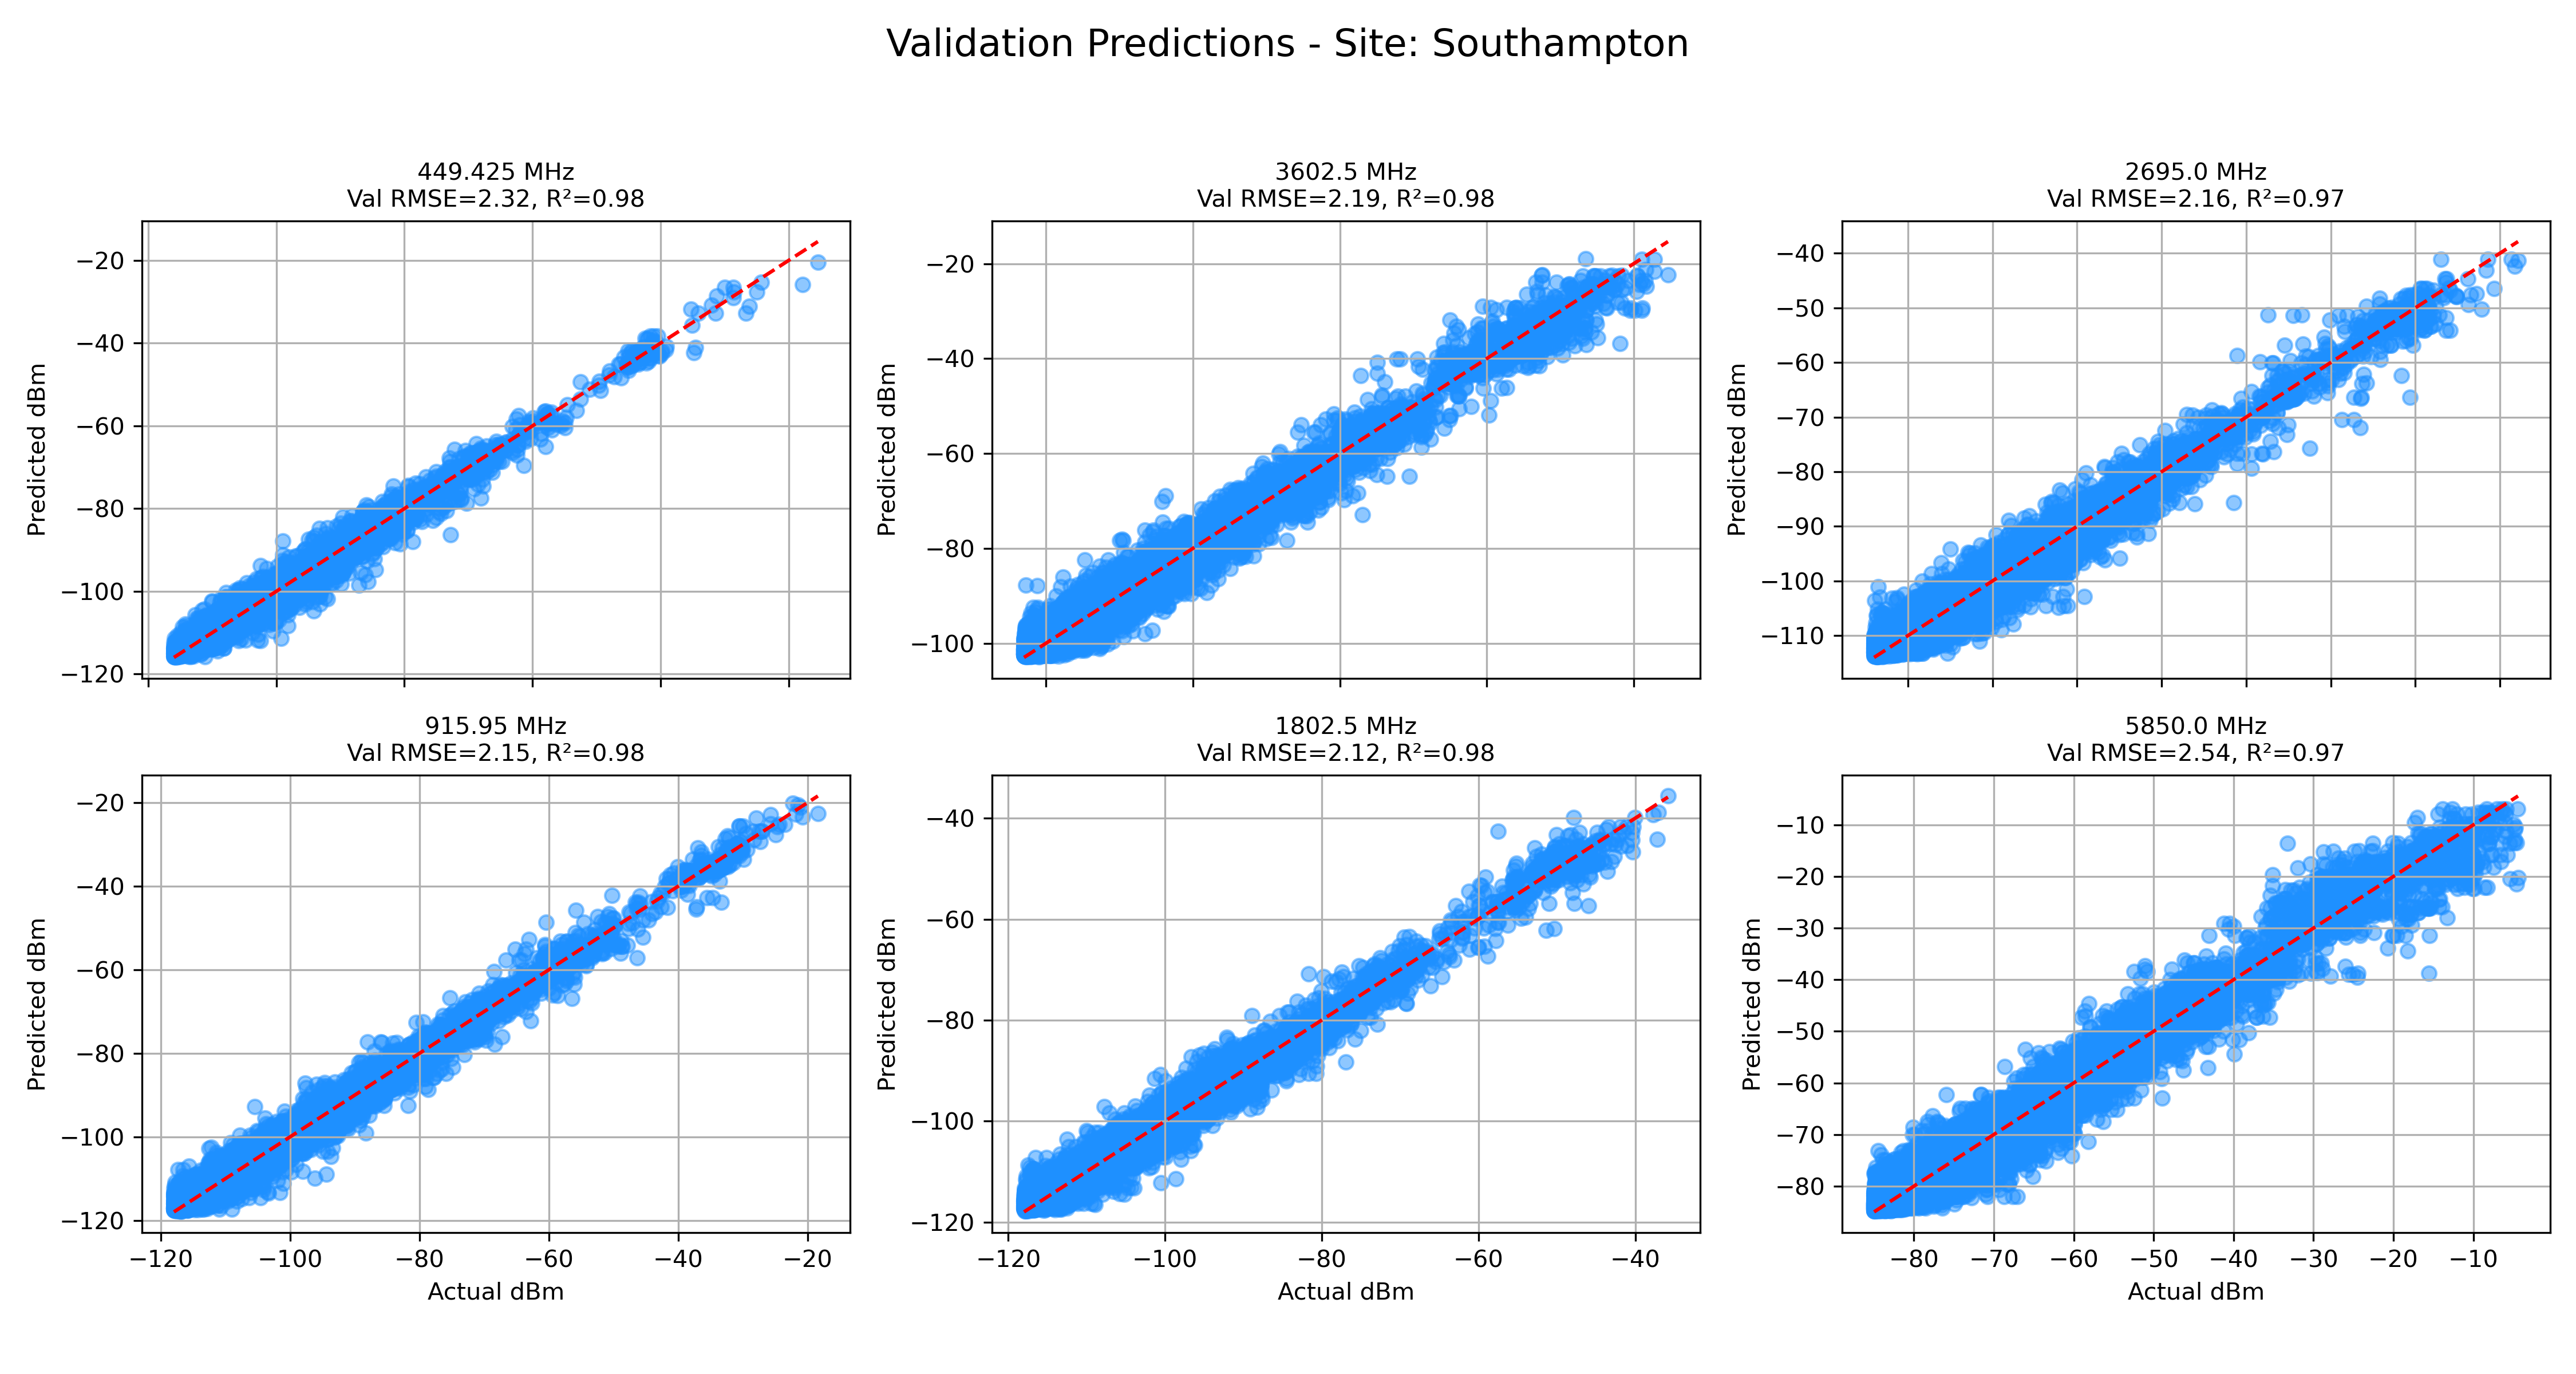
\includegraphics[width=.9\linewidth, height = 0.25\textheight]{Figures/Methodology/RF_F_S_Level/Southampton_val.png}}
    \caption{Validation Results Southampton}
    \label{fig:data-read}
\end{figure}

\begin{figure}[H]
    \centering
    \fbox{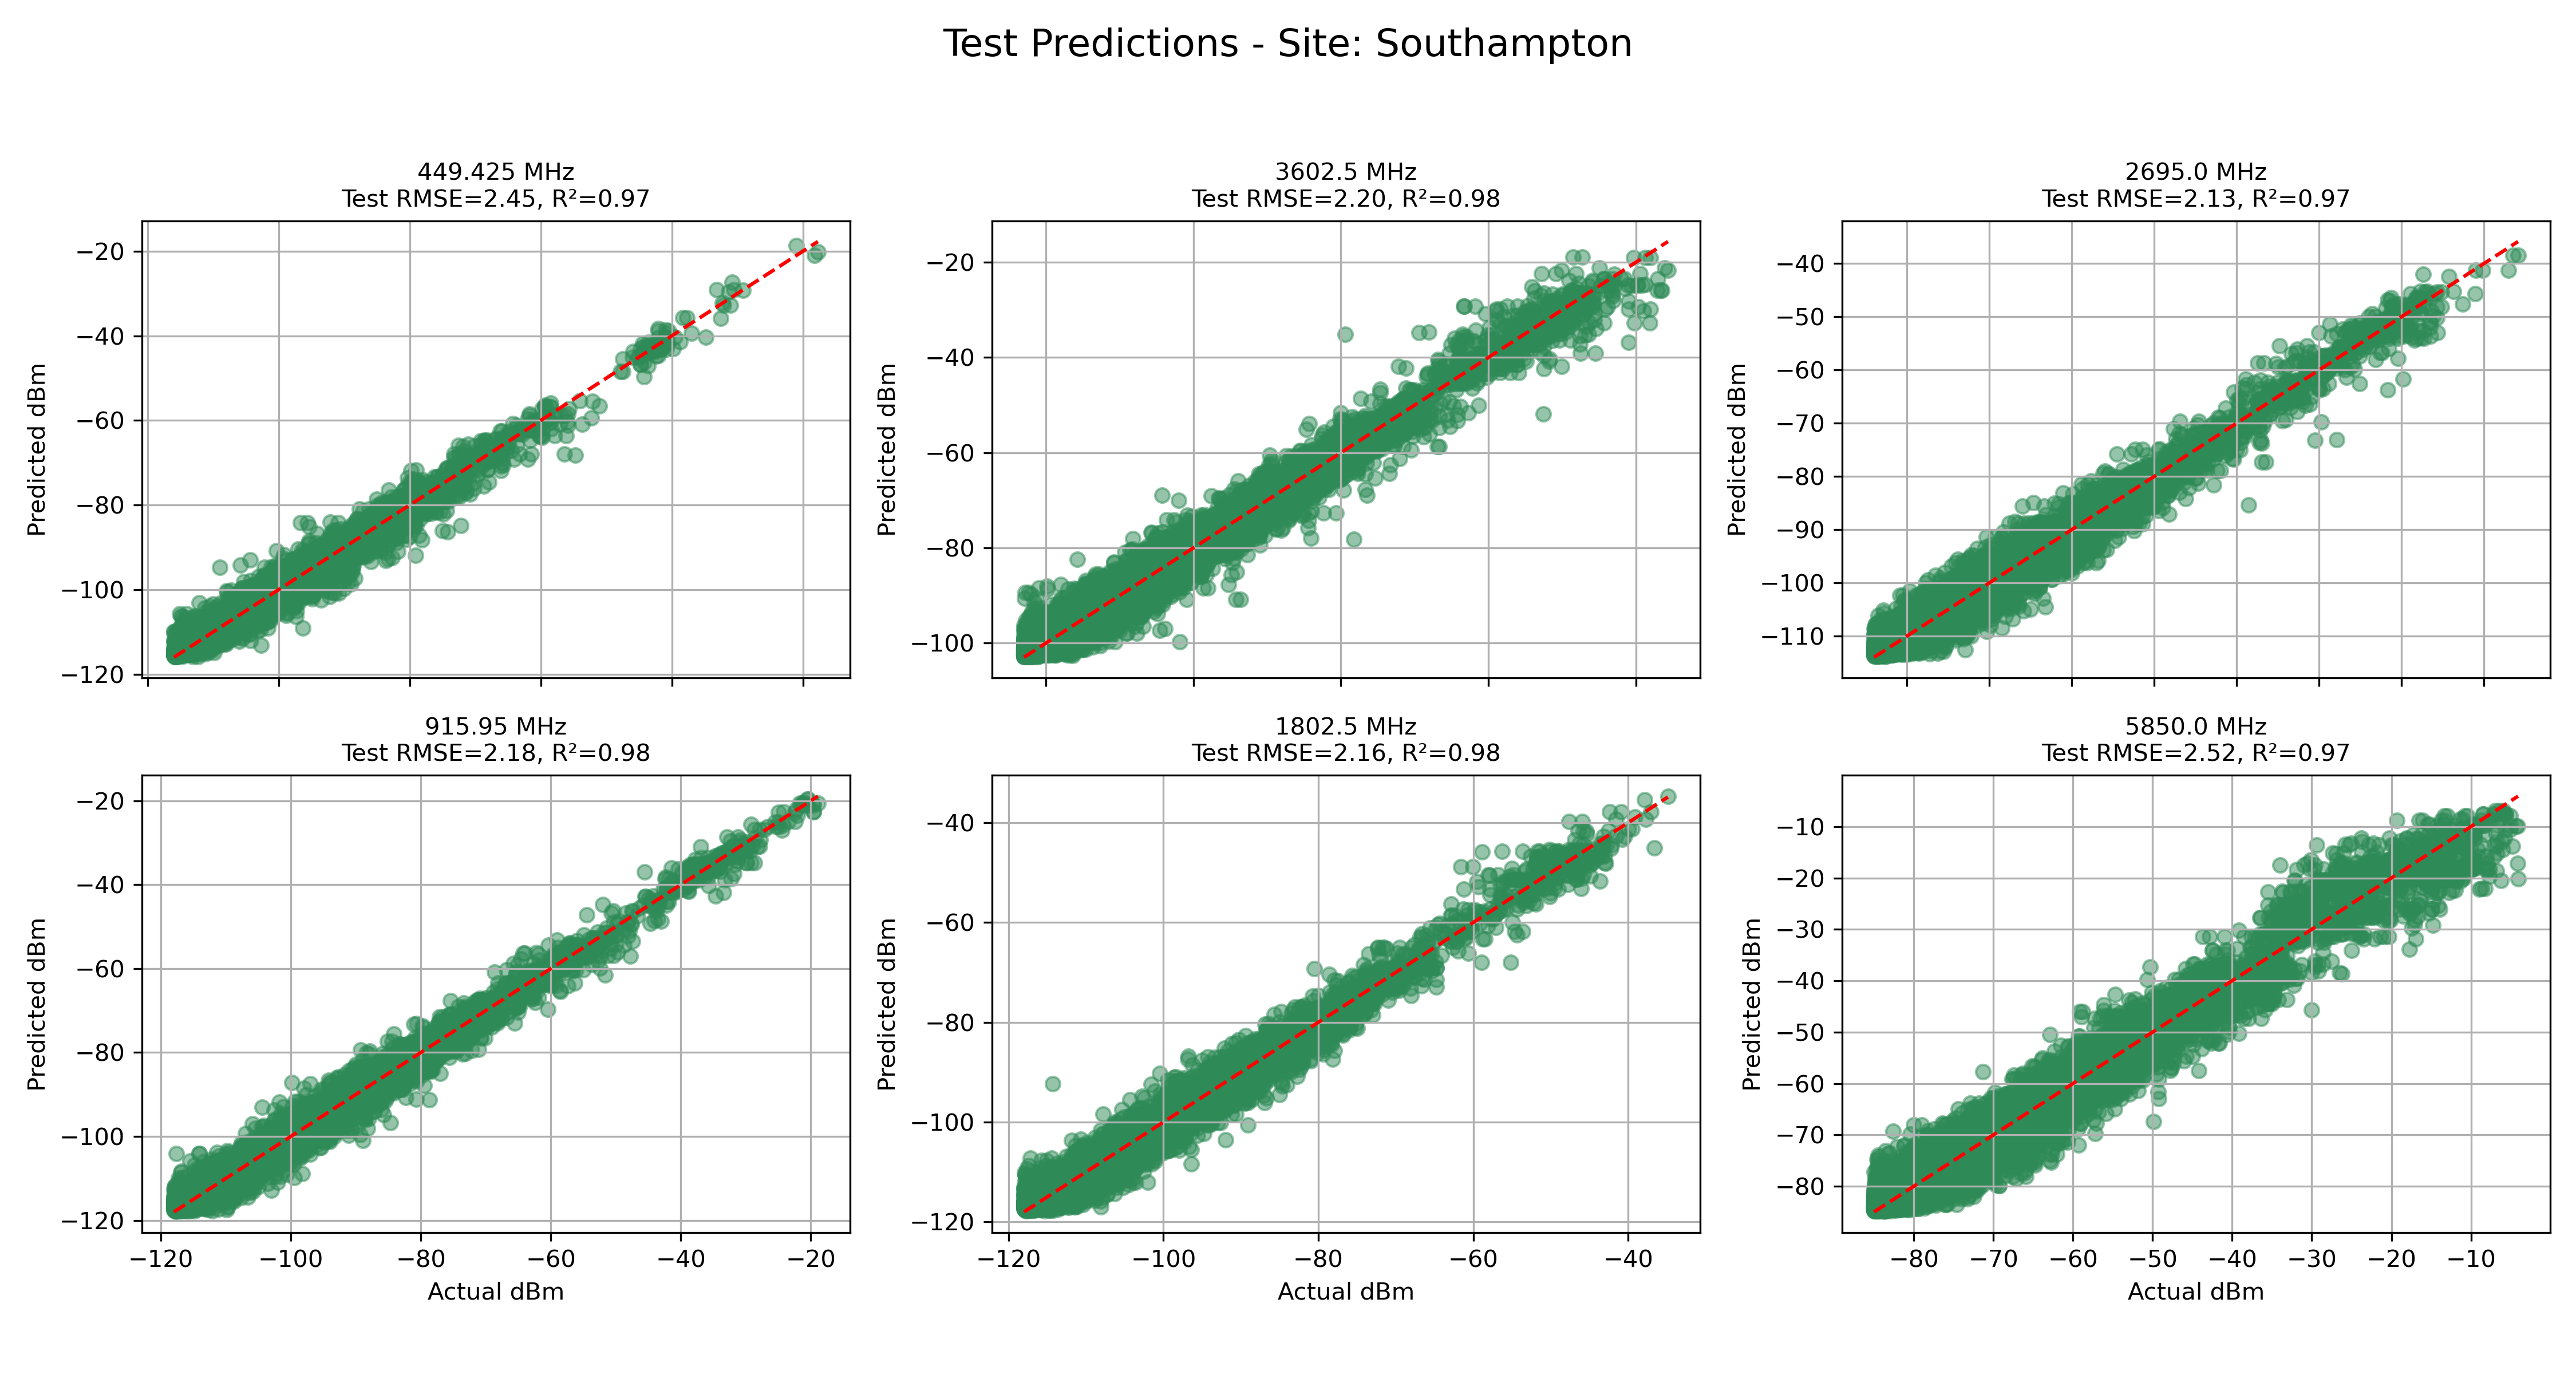
\includegraphics[width=.9\linewidth, height = 0.25\textheight]{Figures/Methodology/RF_F_S_Level/Southampton_test.png}}
    \caption{Test Results Southampton}
    \label{fig:data-read}
\end{figure}

\begin{table}[h]
    \centering
    \begin{tabular}{|c|c|c|c|c|c|}
        \hline
        \rowcolor{myblue}
        \textcolor{white}{\textbf{Frequency (MHz)}} & 
        \textcolor{white}{\textbf{Val RMSE}} & 
        \textcolor{white}{\textbf{Val R²}} & 
        \textcolor{white}{\textbf{Test RMSE}} & 
        \textcolor{white}{\textbf{Test R²}} & 
        \textcolor{white}{\textbf{Num Samples}} \\ \hline
        449.425        & 2.32 & 0.98 & 2.45 & 0.97 & 23,347   \\ \cdashline{1-6}[.4pt/2pt]
        915.950        & 2.15 & 0.98 & 2.18 & 0.98 & 53,597   \\ \cdashline{1-6}[.4pt/2pt]
        1802.500       & 2.12 & 0.98 & 2.16 & 0.98 & 58,092   \\ \cdashline{1-6}[.4pt/2pt]
        2695.000       & 2.16 & 0.97 & 2.13 & 0.97 & 63,942   \\ \cdashline{1-6}[.4pt/2pt]
        3602.500       & 2.19 & 0.98 & 2.20 & 0.98 & 104,213  \\ \cdashline{1-6}[.4pt/2pt]
        5850.000       & 2.54 & 0.97 & 2.52 & 0.97 & 128,458  \\ \hline
    \end{tabular}
    \caption{Model Performance Results Southampton}
    \label{tab:frequency_stats_1}
\end{table}

\begin{itemize}
    \item \textbf{Observation:} \texttt{Figure 5.18}, \texttt{Figure 5.19} and \texttt{Table 5.7} are the model result for site Southampton.
    \begin{itemize}
        \item  Model results remain consistent across the frequency bands with RMSE ranging between $2.13$ to $2.52$ and $R^2 \simeq 0.96$ - $0.98$.  
        \item Some outliers can be observed in some of the frequency bands indicating higher susceptibility to environmental factors.
    \end{itemize}
\end{itemize}

\begin{figure}[H]
    \centering
    \fbox{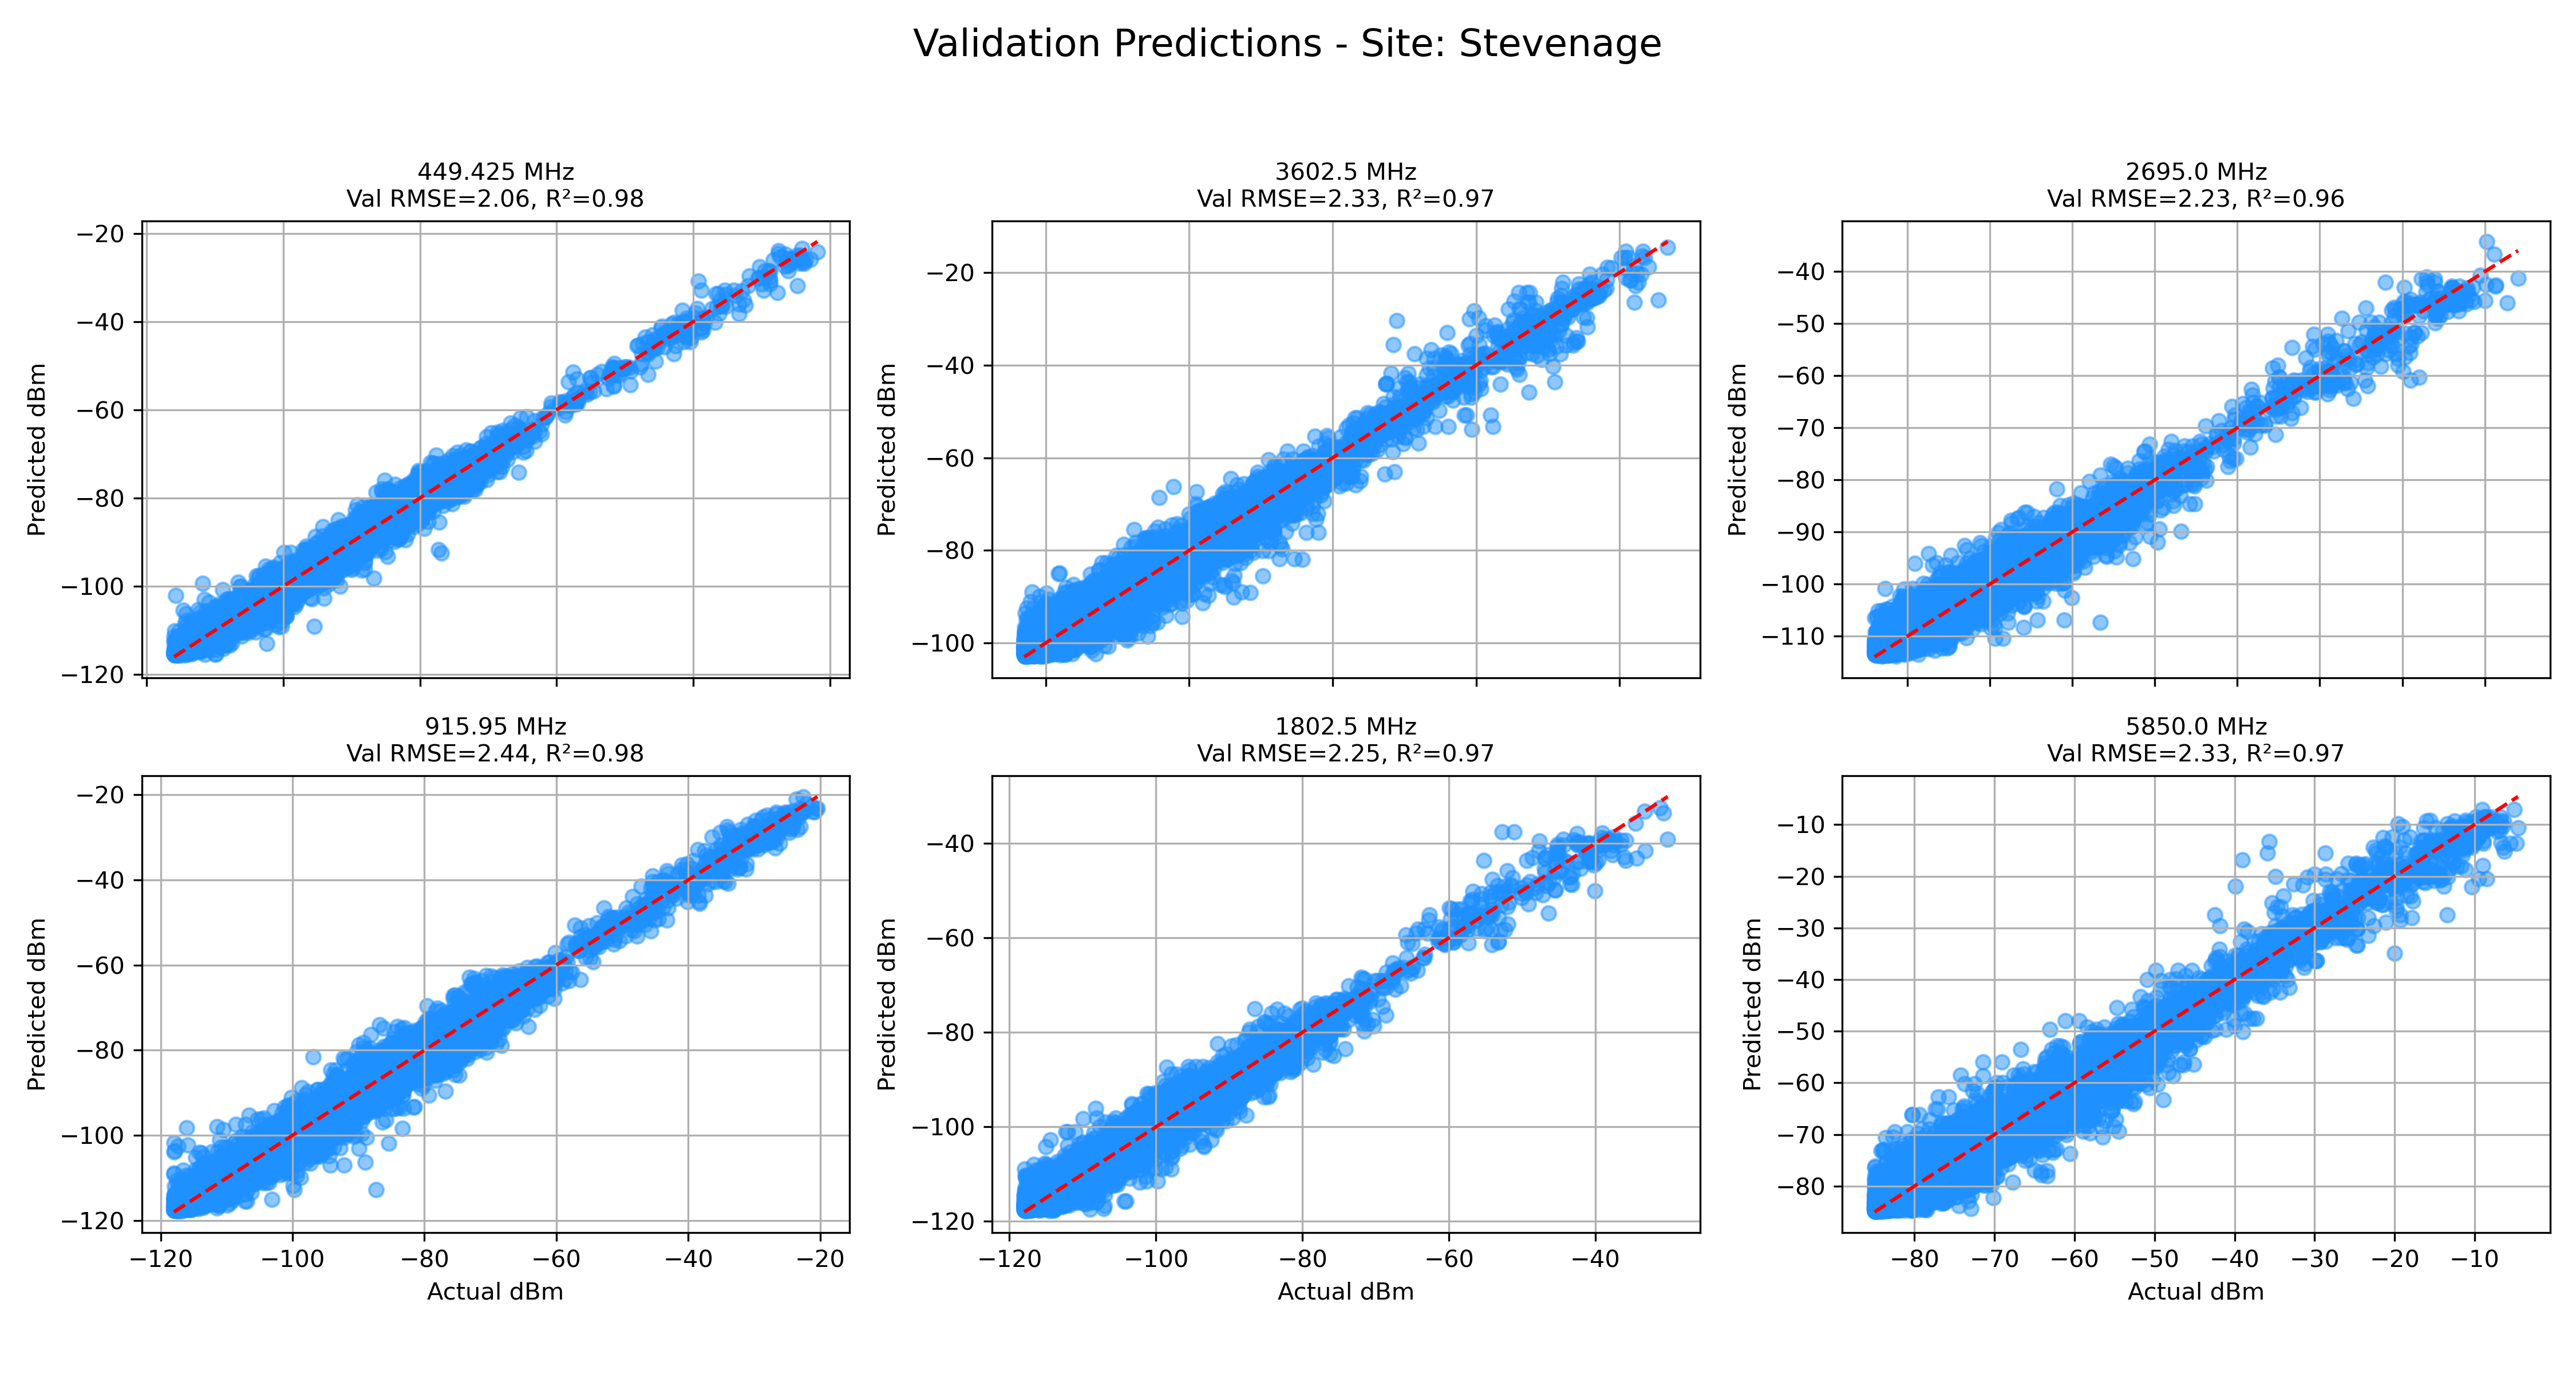
\includegraphics[width=.9\linewidth, height = 0.25\textheight]{Figures/Methodology/RF_F_S_Level/Stevenage_val.png}}
    \caption{Validation Results Stevenage}
    \label{fig:data-read}
\end{figure}

\begin{figure}[H]
    \centering
    \fbox{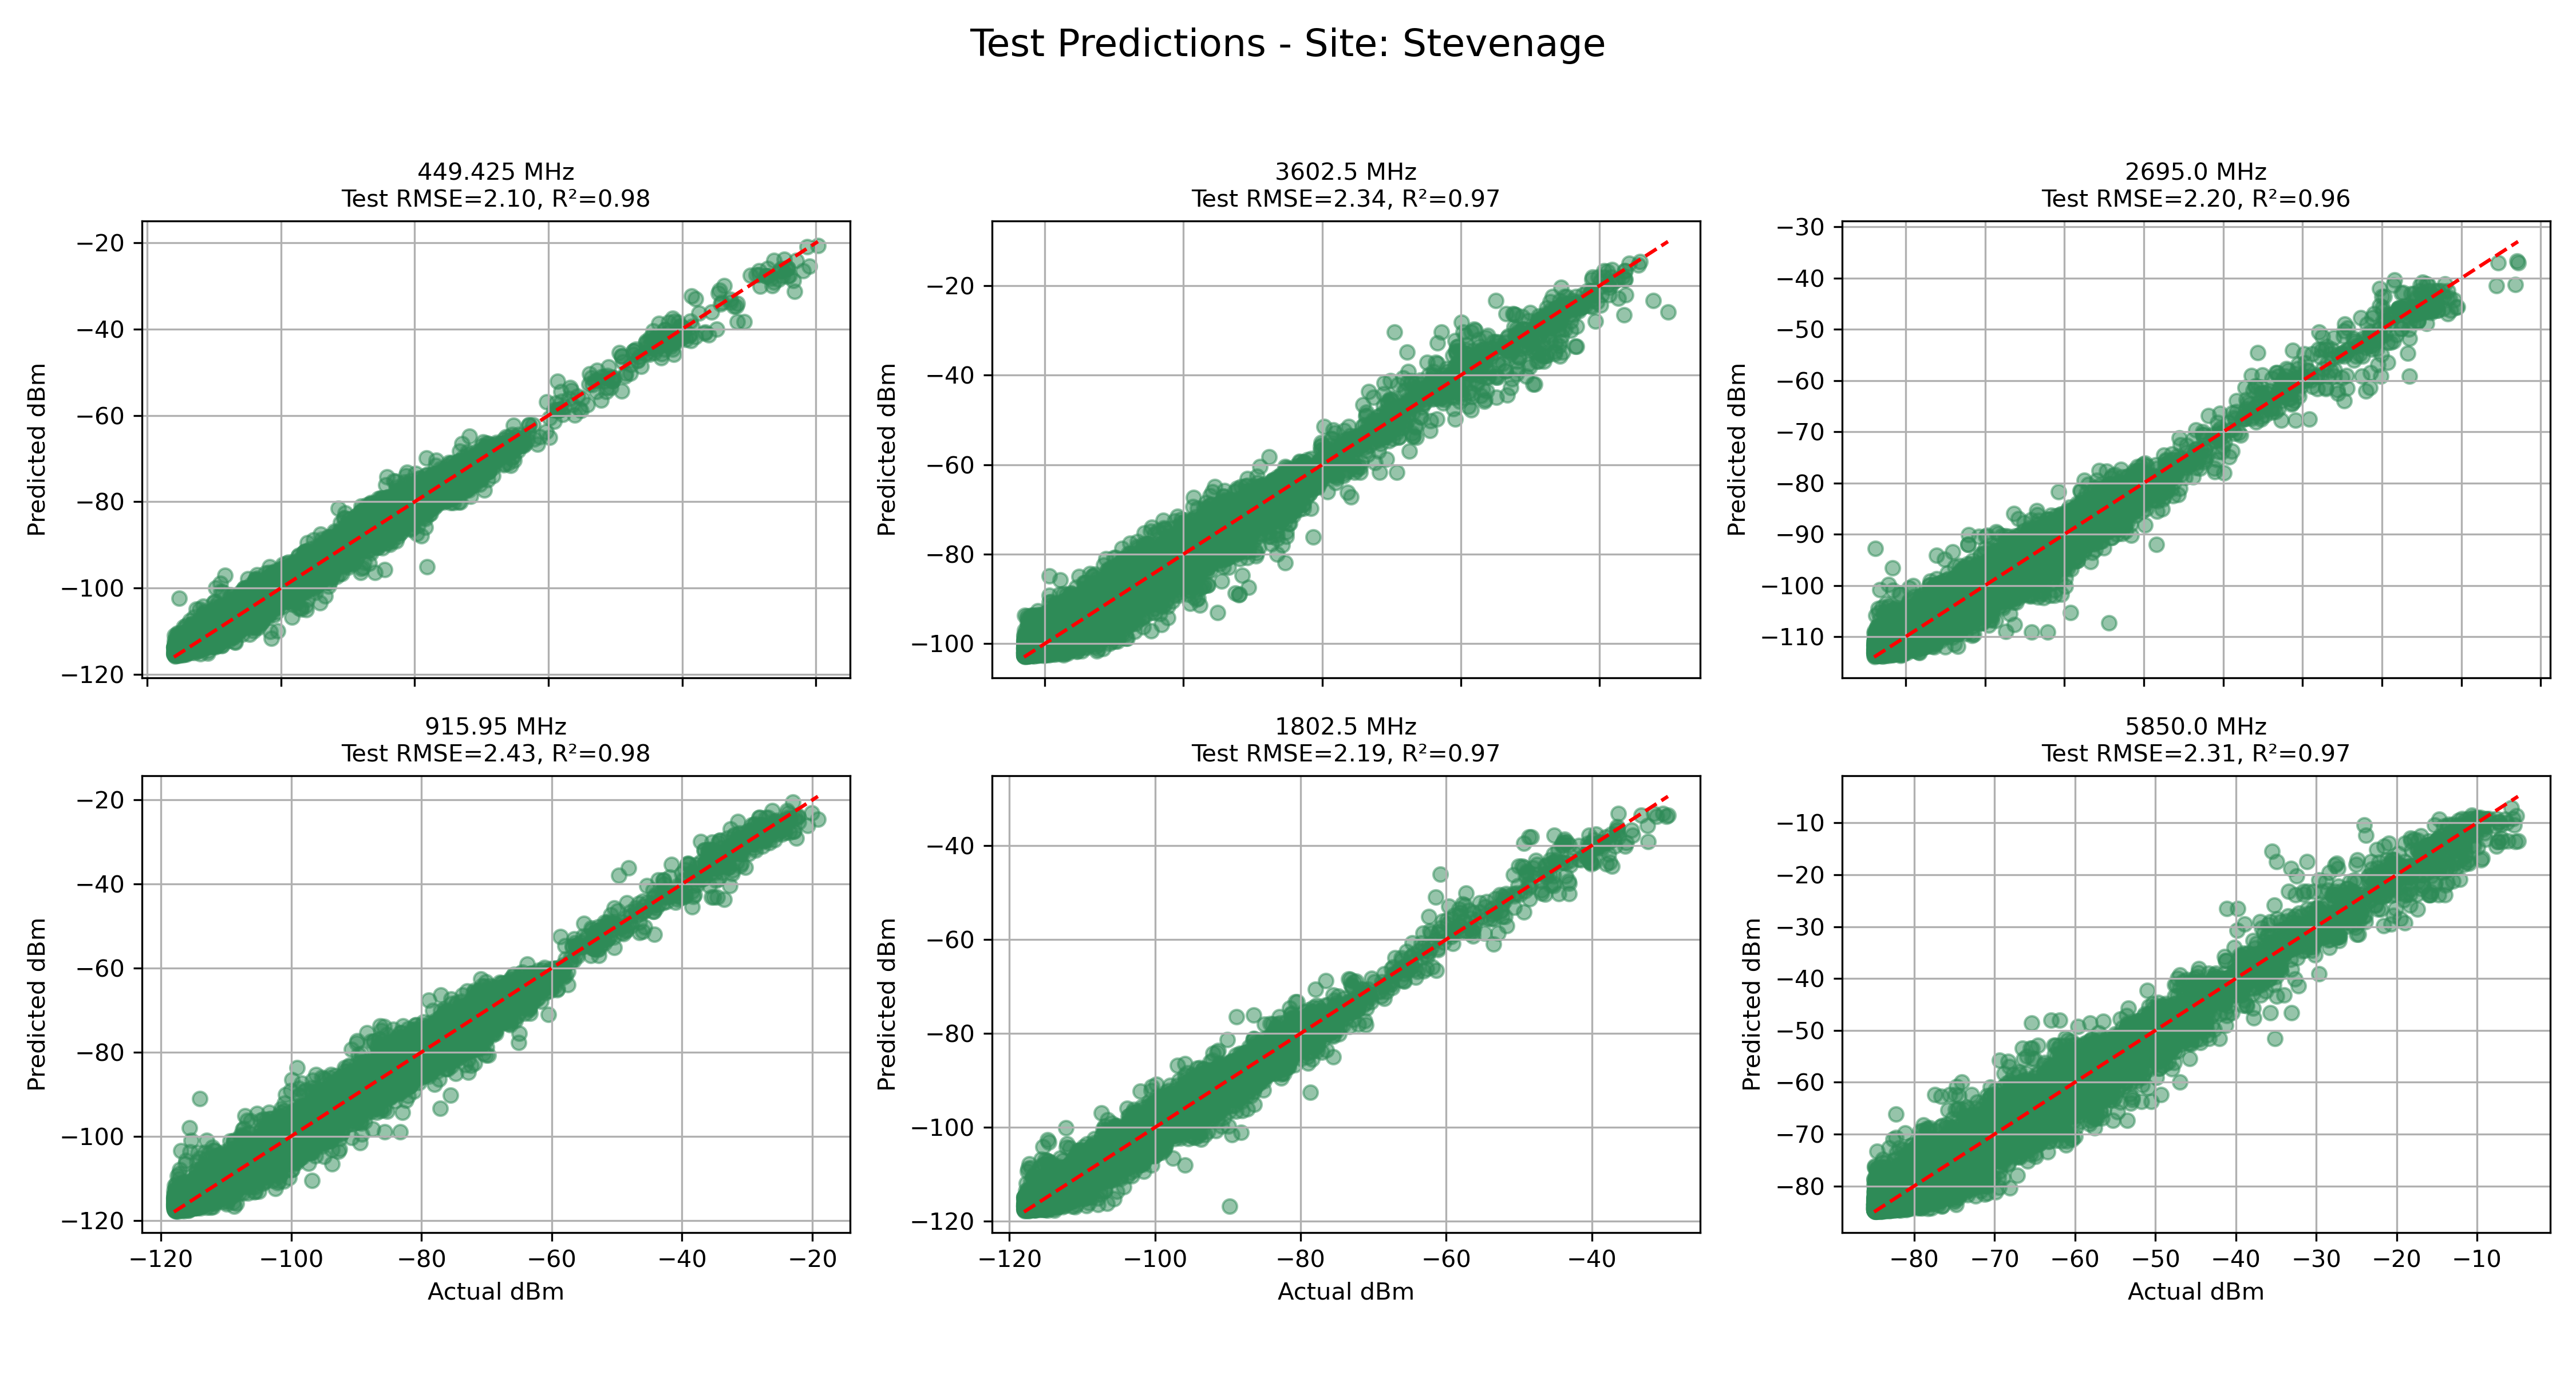
\includegraphics[width=.9\linewidth, height = 0.25\textheight]{Figures/Methodology/RF_F_S_Level/Stevenage_test.png}}
    \caption{Test Results Stevenage}
    \label{fig:data-read}
\end{figure}

\begin{table}[h]
    \centering
    \begin{tabular}{|c|c|c|c|c|c|}
        \hline
        \rowcolor{myblue}
        \textcolor{white}{\textbf{Frequency (MHz)}} & 
        \textcolor{white}{\textbf{Val RMSE}} & 
        \textcolor{white}{\textbf{Val R²}} & 
        \textcolor{white}{\textbf{Test RMSE}} & 
        \textcolor{white}{\textbf{Test R²}} & 
        \textcolor{white}{\textbf{Num Samples}} \\ \hline
        449.425        & 2.06 & 0.98 & 2.10 & 0.98 & 35,439   \\ \cdashline{1-6}[.4pt/2pt]
        915.950        & 2.44 & 0.98 & 2.43 & 0.98 & 71,997   \\ \cdashline{1-6}[.4pt/2pt]
        1802.500       & 2.25 & 0.97 & 2.19 & 0.97 & 45,367   \\ \cdashline{1-6}[.4pt/2pt]
        2695.000       & 2.23 & 0.96 & 2.20 & 0.96 & 53,853   \\ \cdashline{1-6}[.4pt/2pt]
        3602.500       & 2.33 & 0.97 & 2.34 & 0.97 & 94,700   \\ \cdashline{1-6}[.4pt/2pt]
        5850.000       & 2.33 & 0.97 & 2.31 & 0.97 & 105,736  \\ \hline
    \end{tabular}
    \caption{Model Performance Results Stevenage}
    \label{tab:frequency_stats_2}
\end{table}

\begin{itemize}
    \item \textbf{Observation:} \texttt{Figure 5.20}, \texttt{Figure 5.21} and \texttt{Table 5.8} are the model result for site Stevenage.
    \begin{itemize}
        \item  The differences between low and high frequencies are fairly small. The difference in RMSE values only reflects about $2.1$ to $2.4$, suggesting a more homogeneous propagation environment in Stevenage.  
        \item Larger datasets (e.g., 3602.5 MHz with 94k samples and 5850 MHz with 105k samples) are able to keep high accuracy; however, performance trends normalized to sample sizes are consistent over small and large datasets supporting the robustness of the model.
    \end{itemize}
\end{itemize}

\subsection{Overall Insight \& Model Results}

The model maintains a high prediction accuracy and an impressive generalization capability across all sites and frequency bands. Validation and test metrics still closely follow one another, with RMSE not leaving the bounds of 1.8–3.5 dB and $R^2$ never leaving the bounds of $\geq 0.95$, indicating low prediction error, and a very reliable explanation of the variability of the signals strength.

The best performance occurs at lower frequency bands (i.e. 449 MHz), where attenuation provided by the environment is less severe, higher frequencies show slightly greater RMSE and occasional outliers. Nevertheless, these differences are small, and the model still composes well even in more complicated propagation environments.

In conclusion, the modeling results support that this approach is reliable and generalizable across sites and frequency bands, providing a solid basis for future research that can ultimately be translated to the study of real-world signal propagation.

 % ------------Model Selection Section -----------------   
\section{Deep Learning Model}


\subsection{Deep Learning Models}

Deep learning is a subset of machine learning that employs artificial neural networks (ANNs) with multiple hidden layers to model complex non-linear relationships in data. Unlike traditional models that rely heavily on feature engineering, deep learning methods automatically learn hierarchical feature representations directly from raw or minimally processed inputs \parencite{lecun2015deep, goodfellow2016deep}.

\subsection{Mathematical Formulation}

A feedforward deep neural network can be expressed as:

\[
\hat{y} = f(x; \theta) = \sigma\Big(W^{(L)} \, \sigma\big(W^{(L-1)} \cdots \sigma(W^{(1)}x + b^{(1)})\big) + b^{(L)}\Big),
\]

where \(x \in \mathbb{R}^d\) is the input vector (e.g., frequency, distance, environmental features), \(W^{(l)}\) and \(b^{(l)}\) are the learnable weights and biases of the $l$-th layer, \(\sigma\) denotes a non-linear activation function, and \(L\) is the number of layers. Training involves minimizing a loss function, typically Mean Squared Error (MSE) in regression tasks:

\[
\mathcal{L}(\theta) = \frac{1}{N} \sum_{i=1}^{N} (y_i - \hat{y}_i)^2,
\]

where \(y_i\) are ground truth signal measurements and \(\hat{y}_i\) are predictions. Parameters \(\theta\) are updated iteratively using gradient descent and backpropagation \parencite{rumelhart1986learning}.

\subsection{Neural Networks for Radio Propagation}

Neural networks have been increasingly applied to radio wave propagation modeling, including urban, suburban, and maritime environments. Recent studies demonstrate that feedforward and convolutional neural networks outperform traditional empirical models (e.g., COST-231, Hata) and provide lower prediction errors compared to machine learning baselines such as Random Forests \parencite{mahmud2021artificial, khan2022pathloss, gupta2022pathloss}.

For example, Mahmud et al. \parencite{mahmud2021artificial} showed that ANNs predicted path loss in complex urban environments with higher accuracy than empirical models. Similarly, Khan et al. \parencite{khan2022pathloss} reported that ANN-based models achieved lower RMSE compared to Random Forests in 5G urban microcell environments. Gupta et al. \parencite{gupta2022pathloss} highlighted the scalability of deep neural networks when handling large-scale propagation datasets.

\subsection{Comparison with Random Forests}

Random Forests (RFs) are ensemble methods that combine multiple decision trees to provide robust predictions. While they handle non-linearities well and are relatively interpretable through feature importance measures, they partition the feature space in a piecewise fashion, limiting their ability to capture smooth complex interactions across high-dimensional variables \parencite{breiman2001randomforests}.

By contrast, deep learning models approximate highly complex, continuous non-linear functions. In the context of radiowave propagation:

\begin{itemize}
    \item \textbf{Feature Representation:} RFs rely on manual feature engineering, whereas ANNs learn feature hierarchies automatically.
    \item \textbf{Data Scale:} RFs perform well on medium-sized datasets, but ANNs improve as dataset size increases, scaling more effectively.
    \item \textbf{Accuracy:} Empirical results consistently show ANNs outperform RFs in predicting signal attenuation across diverse environments \parencite{mahmud2021artificial, khan2022pathloss}.
    \item \textbf{Interpretability:} RFs are more transparent, while ANNs are often considered ``black-box'' models, though recent explainability methods (e.g., SHAP, saliency maps) help mitigate this issue.
\end{itemize}

\subsection{Summary}

Overall, deep learning provides superior predictive accuracy and scalability for radio propagation modeling, particularly in environments with complex interactions between frequency, terrain, and clutter. Random Forests remain strong baselines, but neural networks demonstrate higher robustness and generalization in large-scale datasets, making them a suitable choice for advanced wireless system design.


In conclusion, deep learning can be used for radio propagation modeling where it achieves superior predictive performance and high scalability, especially in environments with strong coupling between frequency, terrain and clutter. While Random Forests are still strong baselines, the robustness and generalization capabilities of neural networks in large scale datasets makes them an appealing option for advancing contemporary wireless system design.


\subsection{Trained Model \& Results}


\subsubsection{Model Training \& Performance}

    
A neural network (NN) was trained using eight numerical features (e.g. Adjusted e.i.r.p., frequency, Tx–Rx distance, antenna heights, noise floor, site coordinates) and a site embedding factor indicating the transmitting site ID. This enable the model to learn continuous signal related variables as well as site specific characteristics. Distinctions in the site IDs (which show the various location of origins from the matched pairs) were applied to part the dataset into training (80\%) and test(20\%), which is predicated on ensuring that the model generalized to unseen sites than merely memorizing previously observed ones. Overall, around 1.44 million and 0.41 million samples fell out in the training and test sets, respectively. The target variable (received signal strength, Local dBm) had mean of around $–84.68$ dBm and standard deviation of $19.12$ dBm), indicating variation across sites and distances was adequate.

\begin{table}[h]
    \centering
    \begin{tabular}{|c|c|c|}
        \hline
        \rowcolor{myblue}
        \textcolor{white}{\textbf{Model}} & 
        \textcolor{white}{\textbf{MAE}} & 
        \textcolor{white}{\textbf{MSE}} \\ \hline
        \textbf{Neural Network}   & \textbf{8.82}  & \textbf{117.96} \\ \cdashline{1-3}[.4pt/2pt]
        Linear Regression & 10.73 & 188.57 \\ \cdashline{1-3}[.4pt/2pt]
        Random Forest     & 9.89  & 155.02 \\ \cdashline{1-3}[.4pt/2pt]
        XGBoost           & 10.51 & 171.47 \\ \hline
    \end{tabular}
    \caption{Comparison of model performance on the test set}
    \label{tab:model_comparison}
\end{table}

Based on \texttt{Table 5.9} it is clearly visible that neural network has performed way better than other machine learning models, by reducing error $\approx 20\%$ compared to linear regression and $\approx 11\%$ compared to Random Forest. 


\subsubsection{Training Dynamics}

\texttt{Figure 5.22} indicates learning curves of loss and MAE (Mean Absolute Error) on both the training and verification set of the neural network across 69 epochs. These training curves show a pretty rapid decline in loss over the first 10 epochs, with the model quickly capturing the underlying data pattern. Though validation curves largely follow the same descending trajectory, some level of variability exists, as is commonly observed with test segments that are typically more complex and have a more diverse range of sites, variability in curves is greater, particularly for unseen sites.

\begin{figure}[H]
    \centering
    \fbox{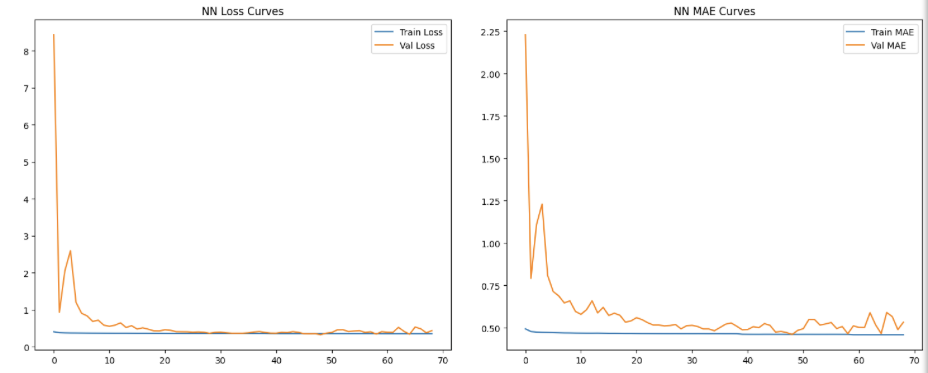
\includegraphics[width=0.9\linewidth]{Figures/Methodology/Deep_L_Model/loss and mae curve.png}}
    \caption{Neural Network Loss Curve \& MAE Curve}
    \label{fig:placeholder}
\end{figure}

We can see that both the training and validation curves start to level out around epochs 40–50, indicating the model has learnt at a fairly stable rate. Crucially, the difference between train and validation performance stays small all along the way, showing no evidence of excessive overfitting. This shows how effective the regularization strategies applied in this case, that is, dropout, batch normalization and L2 regularization, are in improving the generalization of the model.

Additionally, learning rate scheduling mechanism plays crucial role to refine the optimization. The scheduler enabled fine-tuning the model in later epochs with a very low learning rate, thereby preventing divergence and inducing stable convergence as well. In summary, these results underline that the neural network obtained a well-balanced fit capturing complexity without learning noise in the training data.

\subsection{Prediction Accuracy}

\texttt{Figure 5.23} shows Predicted vs Actual signal strengths on test set. It can be clearly seen that Predictions track nearly perfectly along the 1:1 diagonal line, showing high concordance. So, for mid-range values (–110 dBm to –60 dBm) the model strikes pretty close to perfect.

The NN underestimates only high signal strengths (thus strong coverage areas) and overestimates low signal strengths (thus weak coverage areas) at the extremes. This indicates that the model is not able to grasp the more rare extreme cases of the propagation conditions.

\begin{figure}[H]
    \centering
    \fbox{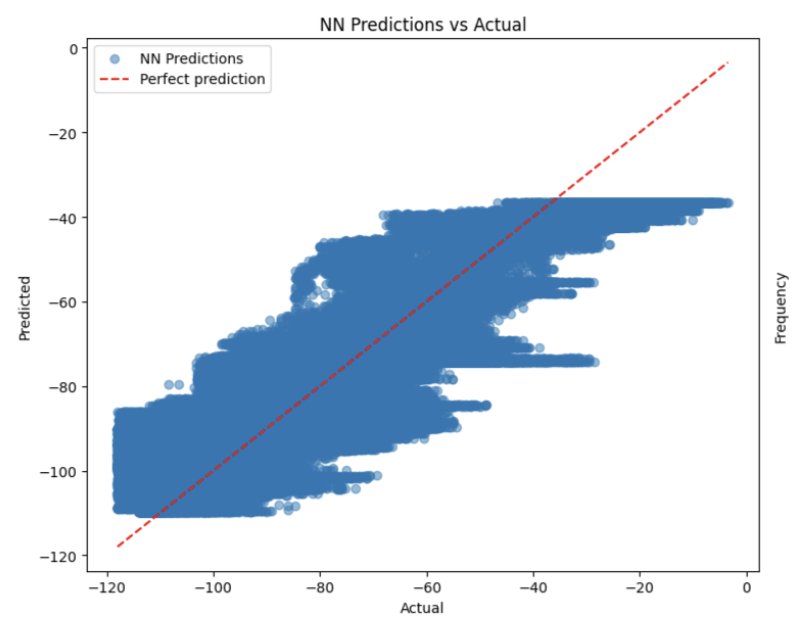
\includegraphics[width=0.9\linewidth, height = 0.3\textheight]{Figures/Methodology/Deep_L_Model/NN_prediction .png}}
    \caption{Neural Network Scatter Plot Actual vs Predicted}
    \label{fig:placeholder}
\end{figure}


As depicted in \texttt{Figure 5.24} where pattern errors are plotted. However, the distribution is a little right skewed, otherwise near a zero center. That means that signal strengths systematically slightly lower.

\begin{figure}[H]
    \centering
    \fbox{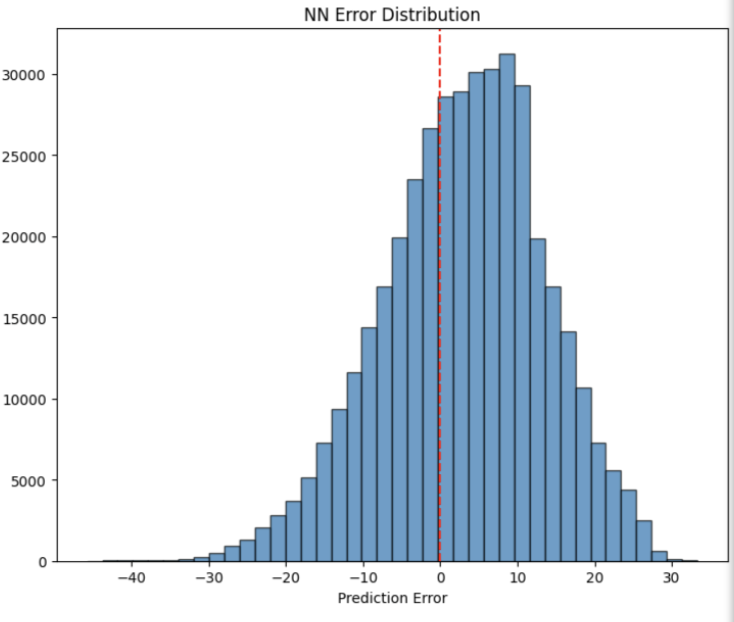
\includegraphics[width=0.9\linewidth, height = 0.3\textheight]{Figures/Methodology/Deep_L_Model/NN_Error.png}}
    \caption{Histogram Neural Network Error Distribution}
    \label{fig:placeholder}
\end{figure}


\subsection{Comparative Baselines}
Although simpler models like Linear Regression served as a quick baseline in our case, they do not capture non-linear dependencies (distance–path loss interactions, to be specific). However, Random Forest gave superior accuracy and was less useful in extrapolating to new sites.

Also, XGBoost despite baing an important algorithm for many tabular problems, it yielded lower scores than the Neural Network, potentially because of the embedding-based NN capturing the complex high-dimensional interactions among the continuous categorical features (site + distances) better than XGBoost.

This shows that deep learning with embeddings is a reasonable choice of architecture for predicting radio signals.




\subsection{Summary of Findings}

Neural Network has performed better than all the other traditional models comparatively across all the evaluation metrics.

\begin{itemize}
    \item Good learning curve indicates well trained model with very minimal overfitting.
    \item Predicted vs Actual plot shows pretty accurate mid range prediction, while having very minimum systematic error at the extreme ends.
    \item Prediction isn't completely unbiased but very close with more than 60\% of the errors within $\pm 10$ dBm as confirmed by error distribution.
    \item In general, the findings validate the practicality of deep learning methods in site-aware signal strength forecasting.
\end{itemize}

 % ------------Model Comparison Section -----------------   
\clearpage
\chapter{Model Selection \& Justification}


Four different models- Linear Regression (LR), Random Forest (RF), XGBoost (XGB), Neural Network (NN), were compared systemically to evaluate the predictive performance of wireless signal strength estimation. For each of these models, we trained and validated on a wide variety of frequency bands, and reported performance measures (in terms of Mean Absolute Error (MAE), Mean Squared Error (MSE), Root Mean Squared Error (RMSE), and R\^2). The results provide valuable information on he pros and cons of each method.

As the simplest baseline, Linear Regression assumes a linear relation between the associated features and signal strength. It is an unreasonable assumption in wireless propagation, empirical laws tell us that signal attenuation is dominated by non-linear effects like multiple path reflections, scattering, and diffraction\parencite{rappaport2017smallscale}. As expected, linear regression performed weakest (10.73 MAE, 188.57 MSE) always coming in last in every frequency band. Though it gives us a useful baseline, linear regression fails to capture the nature of the underlying data, which means it is not suitable for real-world deployment.

An ensemble of decision trees, Random Forest outperformed linear regression. Being non-linear, it could fit capture interaction between features and had lesser error metrics (MAE 9.89, MSE 155.02). The model did, though, overfit the training data a bit, as can be seen by the mild fluctuations of the test metrics at higher frequencies. Indication of the above is that although this model is good at generalizing over linear regression, the majority vote via trees forces random forest to downplay key local structures, which is effectively giving the high-dimensional or frequency sensitive features too much weighting or penalization under high dimensional/ low dimensional circumstances.

Gradient–boosted tree model (XGBoost) gave an almost indistinguishable result as RF (MAE 10.51, MSE 171.47). The predictive accuracy usually improves because each tree in boosting focuses on and sequentially corrects the errors made by the previous trees\parencite{mason2000boosting}. In this case, however, extra complexity of boosting does not turn into a real gain. The XGBoost model performed dependably at all frequencies but still lagging behind the Neural Network. Even tree-based methods can only discern complex non-linear structures strong enough it appears tree-based models are too weak for the task of dynamic device positioning on the whole continent and all the sporadic reflections and dynamics of wireless signal propagation plans the same, i.e. signal parameters, that compose the problem.

The overall error metrics achieved by the Neural Network model show a significant performance when compared with the other models investigated (MAE = 8.82, MSE = 117.96). Even across both validation and test sets, it was able to predict signal strength reliably, maintaining a low absolute error. The model architecture that facilitated learning of hierarchical feature representations allowed the model to learn fine grained propagating characteristics, such as frequency dependent attenuation and variability introduced by complex environments. Most importantly, there was no evidence of overfitting, the validation performance tracked the training performance closely throughout.

In addition to the default (RF) model two additional, distinct configurations of Random Forest model (Model 1 \& 2) trained with hyperparameter tuning to risk prediction for patient separated for tuning and performance estimation were also used.

Random Forest Model 1 (Frequency Level) had a lower number trees along with a default maximum depth to maintain a parameterization level. Whilst this model encompassed large, bold features of the dataset it did not capture subtle distinctions, such as when differentiating between signals, especially at higher frequencies where the attenuation signature becomes more chaotic. Consequently, Model 1 has weaker ability to generalize than NN.

Random Forest Model 2 had trees that went deeper, along with a bigger ensemble. In the mid frequency ranges (915 MHz and 1800 MHz) where, we expect to see the most effect from the additional multipath reflections and scattering effects, this model performed significantly better than Model 1. Although Model 1 is an example of a relatively strong Random Forest, Model 2 showed a more stable test performance and lower variance between the validation and test error which shows that careful tuning of the tree depth and ensemble size can help to boost the RF predictive power somewhat.

However, even with this refinement both RF Model 1 and Model 2 still performed worse than the Neural Network, despite this fine-tuning. While RF error plateaus at higher levels with significant noise across the validation curves, particularly in the upper frequency bands ($\geq 2695$ MHz), Neural Network types yielded steadily lower error across frequency bands (MAE 8.82, MSE 117.96). Even in Model 2, the model limits came from overfitting of the local structures with the RF models, and failure to capture global frequency-dependent interactions.

The comparative analysis illustrates that even if Random Forest and XGBoost provide an intermediate boost against linear regression, they are still limited in capturing highly non-linear relationships. Neural Network showed consistent better metric performance with strong generalization ability and stability, representing a very relevant approach for the wireless signal prediction tasks.

So here, the Neural Network stands out as the most optimal for use case, with its impressive accuracy, good generalization (which is mandatory in this case) and also its expressible nature to fit real world through wireless propagation modeling.

 % ------------Conclusion Section -----------------   
\clearpage
\chapter{Conclusion}

This Report aimed to assess machine learning and deep learning approaches for wireless a signal strength predicting with a special focus on a comparative performance of Random Forest models and Neural Networks. The primary objective was to identify which methods are the most effective at replicating the ability of sound to propagate through the complex dynamics across multiple frequency bands and sites.

The Random Forest models have contributed to the understanding of wireless propagation behavior more effectively. For the frequency-band specific analysis, Random Forest Model~1 (frequency level) and Model~2 (site \& frequency level) produced consistently high predictive performance with RMSE ranging from $2.5$--$3.2 \,\text{dB}$ and $R^{2}$ values between $0.95$--$0.98$ across both validation and test sets. The fact that Random Forests generalize fairly well across frequency bands with minimal predictive error suggests that RMSE may not be distributed evenly across frequency bands, as one might expect under a purely random assumption of cross-compatibility. Interestingly, the frequency decomposition indicated that Random Forests perform better at lower frequencies (i.e., at $449 \,\text{MHz}$ and $915 \,\text{MHz}$). This observation is physically reasonable, since lower frequencies are less susceptible to environmental losses and multipath propagation phenomena. In contrast, Random Forests were somewhat more error-prone and unstable at higher frequencies ($\geq 1800 \,\text{MHz}$), reflecting the increased complexity of propagation mechanisms at these levels. The comparison between Model~1 and Model~2 further demonstrated how design choices (e.g., feature treatment or hyperparameter tuning) can appreciably influence performance, providing a richer view of ensemble tree models in this domain.

The neural network, exceeding the baseline measures, illustrated the highest overall predictive performance. It achieved lowest combined aggregate error metrics throughout the study (MAE = 8.82, MSE = 117.96) and showed no overfitting effect, plateauing training and validation losses were tracking closely. While frequency specific RMSE/R² were not reported for the Neural Network, the superior overall accuracy and stability suggest that it captured hierarchical and non-linear interactions within the data that tree-based methods would be unable to discover. The model represented fine-grained and broad-scale propagation effects with high levels of explanatory power across diverse conditions due to the deep architecture.

The Random Forest and Neural Network models also feature two contrasting complementary strengths: Random Forests offer interpretable results and strong stability of band-wise contiguity while being frequency specific. On the other hand, the Neural Networks convey the best overall accuracy and provide generalization for aggregate performances. Therefore, in terms of practicality here, this indicates that ensemble tree models may provide comparable robustness and interpretability to professionals in unit locations where frequency specific performance is critical, whereas Neural Networks show the ability to generalize across various deployment conditions and scales and provide a path for extremely accurate wireless propagation modeling.


In summary, this report confirms Random Forests are both trusty and explainable frequency wise prediction models, and shows that despite their quite stable and the high accuracy value and good performance, the best overall performance is achieved by aggregation of the Neural Network sets. Collectively, these insights offer a solid framework for future studies as well as practical applications in the field of spectrum management, wireless network planning, and signal propagation modeling.

 % ------------Future Enhancements Section -----------------   
\clearpage
\chapter{Future Enhancements}

The current work shows that deep learning has the potential to predict accurately and in a generalizable manner radio wave propagation across frequency bands, but there are multiple possibilities to extend and improve the approach in future studies.

\section{Embedding of Topographic and Environmental Features}

A major improvement would be the incorporation of more granular topographic and environmental data like elevation, land use, building density, and vegetation cover. Radio signals essentially have very poor propagation characteristics due to terrain and obstructions, and such considerably spatial context could be included to enable the model to learn attenuation effects that could not be explained by radio frequency alone. The prediction framework may be tailored for accounting the shadowing, diffraction and multi-path phenomena by incorporating other features such as digital elevation models (DEMs) or geographic information system (GIS) layers. Doing so will not only improve accuracy but also enhance the practical applicability of model planning for real world deployment in urban and rural contexts.

\section{Advanced Outlier Detection and Removal}

The existing analysis shows that there are some outliers that could be due to measurement noise, site specific effects, or particularly extreme propagation conditions. These data points are sparse but can still affect the model fit, even at a higher frequency, leading to bad performances. While future efforts should focus on developing robust outlier detection and removal methods via statistical thresholding, clustering-based anomaly detection, or autoencoder-based reconstruction errors. The model can then have lower error variance and produce better predictions, across sites, after systematically identifying which values are spurious and excluding them prior to training. Learning about the reasons behind these outliers, either environmental conditions affecting the detection, or maybe an instrumentation error, can serve as a valuable ground to improve data collection protocols.

\section{Rebuild Deep Learning Models at Various Levels of Granularity}

Another most important next step for this analysis is the redevelopment of deep learning architectures that run at different granularity. Model is trained in a global environment across sites and assemblies, epoch based on current framework. On the other hand, training specialized model at a more finer granularity (i.e. frequency-specific or site-specific as well as environment-type specific (urban, submerged, rural)) might be better able to capture unique propagation properties. Another alternative to explore would be a multi-task learning approach, with a common neural backbone across all tasks learning common representations while separate branches compactly model granular variations. In addition, a hierarchical deep learning model that combines coarse-grained generalization with fine-grained adaptation may be employed. This would strike a better balance between model robustness and capturing subtle environmental or frequency-dependent effects, thereby leading to a more flexible and scalable prediction model.

To conclude, consideration of different components considered for enhancing the model with the purpose of integration of topographic information, systematic outlier handling and deep learning architectures at finer levels would help achieve not only better accuracy but also better applicability of prediction over diverse, real-world propagation environments. These guidelines give a solid reference for further investigation and implementation for communication system design and operation.

 % ------------References Section -----------------  
\clearpage  % Forces a new page
\phantomsection % Important for hyperref to link correctly
\addcontentsline{toc}{chapter}{\textbf{References}} % Bold entry in TOC
\renewcommand{\bibname}{References} 
\printbibliography
\clearpage
\end{document}




% Reprase the data description portion
